\documentclass[11pt]{article}
\usepackage[T1]{fontenc}
\usepackage{lmodern}
\usepackage[margin=1.05in]{geometry}
\usepackage{amsmath,amssymb,amsthm,mathtools}
\usepackage{microtype}
\usepackage{longtable,booktabs}
\usepackage{tikz}
\usetikzlibrary{arrows.meta,positioning,calc}
\usepackage{xcolor}
\usepackage{xurl}
\definecolor{linkblue}{RGB}{20,69,103}
\usepackage[colorlinks=true,linkcolor=linkblue,citecolor=linkblue,urlcolor=linkblue]{hyperref}
\hypersetup{pdftitle={Conditional information under deterministic coordinate sweeps},pdfauthor={OpenAI},bookmarksopen=true,bookmarksopenlevel=1,bookmarksnumbered=true}

\newlabel{f-shear:lem:delayed-symmetry}{{10.1}{}{}{}{}}
\newlabel{h-lem:path-cylinder}{{3.1}{4}{}{}{}}
\newlabel{h-lem:sequential-tv}{{4.1}{6}{}{}{}}
\newlabel{l-l:central-projector-operator}{{4.5}{12}{}{}{}}
\newlabel{l-l:character-lift}{{7.3}{20}{}{}{}}
\newlabel{l-l:coarse-character-lift}{{4.4}{12}{}{}{}}
\newlabel{l-l:coefficient-average}{{C.1}{62}{}{}{}}
\newlabel{l-l:coefficient-lift}{{4.4}{12}{}{}{}}
\newlabel{l-l:coefficient-operator}{{4.2}{11}{}{}{}}
\newlabel{l-l:degree-all-powers}{{6.3}{17}{}{}{}}
\newlabel{l-l:degree-inverse-square}{{A.2}{54}{}{}{}}
\newlabel{l-l:degree-reciprocal-two}{{A.2}{54}{}{}{}}
\newlabel{l-l:degree-sqrt-deficit}{{A.6}{58}{}{}{}}
\newlabel{l-l:domain-transfer}{{10.4}{35}{}{}{}}
\newlabel{l-l:eight-block-probe}{{8.4}{23}{}{}{}}
\newlabel{l-l:forest-bulk}{{14.3}{47}{}{}{}}
\newlabel{l-l:forest-clipping}{{14.1}{46}{}{}{}}
\newlabel{l-l:forest-hybrid}{{14.4}{48}{}{}{}}
\newlabel{l-l:four-block-reservoir}{{8.3}{22}{}{}{}}
\newlabel{l-l:four-coefficient}{{C.3}{63}{}{}{}}
\newlabel{l-l:isotypic}{{3.5}{9}{}{}{}}
\newlabel{l-l:joint-type-operator}{{8.2}{22}{}{}{}}
\newlabel{l-l:joint-types}{{8.1}{21}{}{}{}}
\newlabel{l-l:orbit-average}{{C.2}{63}{}{}{}}
\newlabel{l-l:orbit-span}{{3.2}{7}{}{}{}}
\newlabel{l-l:palette-information}{{12.1}{39}{}{}{}}
\newlabel{l-l:palette-transfer}{{12.4}{42}{}{}{}}
\newlabel{l-l:peeling-lift}{{C.6}{65}{}{}{}}
\newlabel{l-l:random-partition}{{5.1}{13}{}{}{}}
\newlabel{l-l:replica-clipping}{{13.1}{44}{}{}{}}
\newlabel{l-l:signed-palette}{{12.3}{41}{}{}{}}
\newlabel{l-l:three-group}{{9.2}{28}{}{}{}}
\newlabel{l-l:trim}{{2.3}{5}{}{}{}}
\newlabel{l-l:two-sided}{{8.5}{24}{}{}{}}


\newtheorem{theorem}{Theorem}[section]
\newtheorem{lemma}[theorem]{Lemma}
\newtheorem{proposition}[theorem]{Proposition}
\newtheorem{corollary}[theorem]{Corollary}
\theoremstyle{definition}
\newtheorem{definition}[theorem]{Definition}
\theoremstyle{remark}
\newtheorem{remark}[theorem]{Remark}
\DeclareMathOperator{\KL}{KL}
\newcommand{\F}{\mathbb F_2}
\newcommand{\E}{\mathbb E}
\newcommand{\TV}{\mathrm{TV}}
\newcommand{\op}{\mathrm{op}}
\newcommand{\HS}{\mathrm{HS}}
\newcommand{\id}{\mathrm{id}}
\DeclareMathOperator{\tr}{tr}
\DeclareMathOperator{\Sym}{Sym}
\DeclareMathOperator{\Span}{span}
\DeclareMathOperator{\sgn}{sgn}
\newcommand{\one}{\mathbf 1}
\newcommand{\Unif}{\operatorname{Unif}}
\numberwithin{equation}{section}

\title{Conditional information under deterministic coordinate sweeps}
\author{OpenAI}
\date{September 26, 2026}

\begin{document}
\maketitle
\begin{abstract}
We bound the information remaining after paths of specified cards in the Thorp shuffle on $n=2^d$ cards have been observed. After a fixed number of deterministic coordinate sweeps, the joint endpoint law of further cards is close to uniform on the available positions, on average over the observed paths, provided a fixed positive fraction of labels lies outside both lists. Combined with a Fourier transfer, these bounds give full-deck mixing after $2048d$ physical shuffles.
\end{abstract}
\begingroup
\small
\tableofcontents
\endgroup
\section{Introduction}

What remains random in a shuffle after the paths of many cards have
been observed? For the Thorp shuffle, the answer is especially concrete.
On a pair containing two unobserved positions, the conditional masses
of an additional card are averaged. On a pair containing one observed
position, the remaining mass is transported to the uniquely available
output. Observing more paths therefore changes an averaging process
into a random mixture of averaging and transport. This paper estimates
the information retained by that conditional process.

The positions are the vertices of $V=\mathbb F_2^d$, with $n=2^d$.
One physical Thorp shuffle independently switches each pair in one
coordinate direction and rotates the coordinates. Undoing these
rotations gives a process $(\Pi_t)$ that uses the coordinate directions
in a fixed cyclic order. A sweep consists of $d$ such layers, hence
$d$ physical shuffles. We label cards by their initial positions;
$\Pi_t(a)$ is the position of card $a$ at time $t$. All starting
decks considered below are deterministic. Total variation has the
normalization $\|\mu-\nu\|_{\TV}=\frac12\sum_x|\mu(x)-\nu(x)|$.
Write $q_d$ for the law of one physical shuffle on $S_n$ and $U_{S_n}$
for the uniform law. The threshold-$1/4$ mixing time is
\[
 t_{\mathrm{mix}}(d)=\min\{t\in\mathbb Z_{\ge0}:
          \|q_d^{*t}-U_{S_n}\|_{\TV}\le1/4\}.
\]
Convolution represents independent successive shuffles. Relabeling
the deterministic starting deck leaves its distance from uniform unchanged.

Thorp introduced the shuffle in a study of nonuniform human shuffling
and its consequences for Faro~\cite{thorp,morris44}. Its simple description
conceals a difficult full-deck mixing problem: the transitions are
nonreversible, and uniformity of individual card positions does not
control their joint order. Morris's first polynomial bound for $n=2^d$,
circulated in 2005 and published in 2008, gave $O(d^{44})$ physical
shuffles~\cite{morris44}. His proof combined evolving sets with a
chameleon process for a forward--backward version of the shuffle.
Montenegro and Tetali retained Morris's contraction estimate and
sharpened the mixing analysis using spectral profiles and evolving
sets, obtaining $O(d^{29})$ in 2006
\cite[Theorems~6.14--6.15]{montenegro-tetali2006}.

Morris subsequently developed an entropy method that reduces mixing
estimates to local interactions between pairs of cards. It yielded
$O((\log n)^4)$ physical shuffles for every even $n$~\cite{morris4},
followed by $O(d^3)$ for $n=2^d$~\cite{morris3}. These arguments
decompose the entropy of a permutation into conditional one-card
contributions and analyze the reverse shuffle. They make explicit
why information remaining after other cards are exposed is central
to the full-deck problem.

Ordered Thorp marginals also arise in the small-domain enciphering
analysis of Morris, Rogaway and Stegers~\cite[Theorem~1]{mrs}.
For each fixed $0<\varepsilon<1$, their estimate gives
$O_\varepsilon(d)$ physical shuffles for specified lists of at most
$n^{1-\varepsilon}$ cards.
Czumaj and V\"ocking~\cite{CzumajVocking2014} reached lists containing
any fixed fraction less than one of the deck: a non-Markovian coupling
on butterfly networks gives $O((\log n)^2)$ physical shuffles.
Their full-permutation algorithm adds empty cards and removes them
afterwards; its chain therefore differs from the unchanged labeled
deck considered here.

A closely related conditional-energy strategy appears in the
swap-or-not analysis of Hoang, Morris and Rogaway
\cite[Section~3, Theorem~3 and Lemma~4]{hmr2014}.
They control a centered squared error for the next card and sum the
resulting conditional errors along an ordered list. Their matching
is selected by a fresh uniform group key at each round, and their
contraction is averaged over those keys. Here the coordinate directions
are prescribed cyclically, while the switch coins remain random.
We condition explicitly on preceding cards' complete paths. The
resulting transport-and-average flow admits an exact one-sweep memory
identity, and independent coordinate blocks control its remaining
noise. Thus the common sequential comparison is retained, while the
contraction comes from the geometry of the deterministic schedule.

\paragraph{Conditional information and the first mixing result.}
For a fixed set $B$ of observed labels, let $\mathcal H_t$ record its
paths through time $t$, and let $V_t=V\setminus\Pi_t(B)$ be the
available positions. For a further label $a\notin B$, the basic object is
\[
 f_t(x)=\Pr\{\Pi_t(a)=x\mid\mathcal H_t\}
             -\frac{\one_{V_t}(x)}{|V_t|}.
\]
It is a sum-zero vector supported on $V_t$. Its energy
$\E\|f_t\|_2^2$ controls the expected error in the conditional law
of $a$. Revealing additional cards successively converts this scalar
estimate into information about an ordered list. An average over random
lists need not bound every specified list, and an unconditional marginal
estimate need not survive conditioning on another family of paths.

Our first result gives uniform bounds for specified lists and then
recovers the full permutation. Here $\operatorname{inj}([k],V)$
denotes ordered $k$-tuples of distinct positions.

\begin{theorem}[Fixed lists and a full-deck consequence]\label{thm:first-main}
Uniformly over deterministic starting decks and specified ordered lists
of distinct labels, the following hold as $d\to\infty$:
\begin{enumerate}
\item At time $256d$, the images of any $k\le7n/8$ labels have
total-variation distance $o(1)$ from
$\Unif(\operatorname{inj}([k],V))$.
\item At time $1024d$, the images of any $k\le15n/16$ labels have
total-variation distance at most $n^{-3/2}$, for all sufficiently
large $d$.
\item The full permutation law satisfies
$\|q_d^{*(2048d)}-U_{S_n}\|_{\TV}\to0$.
\end{enumerate}
\end{theorem}

The full-deck conclusion has the optimal order in $d$: the support
of $t$ shuffles has size at most $2^{tn/2}$, which gives
$t_{\mathrm{mix}}(d)\ge2d-O(1)$, whereas the theorem gives
$t_{\mathrm{mix}}(d)\le2048d$ for all sufficiently large $d$.
Section~\ref{sec:prelim} gives the exact lower bound.

Section~\ref{sec:first-route} proves the two fixed-list estimates locally.
For the full-deck conclusion it uses the trimming, isotypic
and reciprocal-degree statements from
\emph{From partial permutation information to Fourier bounds}
\cite{partialFourier}, with their hypotheses stated at the application.
These inputs complete the first route through the paper. The companion
\emph{Optimal-order mixing of the Thorp shuffle}~\cite{optimalThorp}
gives a separate local $1600d$ proof. The $1600d$ application in
Section~\ref{mart:applications} instead uses the Fourier companion's
random-partition transfer.

The first extension keeps paths that have already been observed as
part of the information in the conclusion. Fix $0<p<1$, a set $B$ of
base labels, and a disjoint ordered list $(a_1,\ldots,a_k)$, with
$|B|+k-1\le pn$. Section~\ref{sec:base-paths} proves that a fixed
number $2b(p)$ of sweeps gives, with $T=2b(p)d$, for all sufficiently
large $d$ depending only on $p$,
\[
 \E\left\|
 \mathcal L\big((\Pi_T(a_j))_{j=1}^k\mid\mathcal H_T\big)
 -\Unif\big(\operatorname{inj}([k],V_T)\big)
 \right\|_{\TV}\le kn^{-4}.
\]
Here $\mathcal H_T$ and $V_T$ refer only to the base labels $B$.
The error is averaged over their actual paths; it is not asserted
for every possible history. The estimate holds in either coordinate
order and survives coarsening that retains $V_T$. Its scalar input
allows every deterministic sum-zero vector on the available set, so
the contraction can be restarted at a later observation time.

\paragraph{Why a deterministic sweep contracts.}
Let $i_t$ be the coordinate used at time $t$, and let $P_i$ average
all coordinate-$i$ pairs. The conditional vector obeys
$f_{t+1}=P_{i_t}f_t+\xi_t$, where $\xi_t$ is centered given the
past. The product of a full cycle of $P_i$ annihilates every sum-zero
vector. Thus the present energy consists entirely of noise generated
during the preceding sweep. Each noise contribution has an exact
geometric weight. To bound its size, condition just after the previous
use of the current coordinate. The observed-card densities in its
two halves are nearly balanced, and the intervening switch arrays
in those halves are independent. A squared mass in one half can
therefore be separated from the event that its opposite partner is
occupied. This controls the new noise without replacing the
prescribed directions by independent random directions.

There are two ways to develop this signed flow further.
Sections~\ref{sec:noise-extensions} and~\ref{mart:section} compare
balance for fixed and randomly sampled lists, identify the noise
weights in Walsh coordinates, and construct pointwise endpoint bounds
on events known before the next card is exposed.
Sections~\ref{cycles:section}--\ref{sweeps:section} retain block sums,
variances and pair differences. A first sweep spreads the available
positions and signed mass among coordinate blocks; independent
evolution inside those blocks makes the next sweep contract.
Section~\ref{prefix:section} uses an additional symmetry of the
completed-sweep law to contract after every subsequent sweep, rather
than restarting a two-sweep argument from each realized configuration.

\paragraph{Entropy, simultaneous constraints, and sparse paths.}
The first scalar estimate already gives arbitrarily small inverse-power
relative entropy for every specified list omitting a fixed fraction of
the labels; see \eqref{noise:uniform-entropy}. The later entropy arguments
retain different structure rather than strengthen that conclusion.
Section~\ref{prefix:section} keeps the contribution of each level in a
coordinate-block hierarchy. Section~\ref{lifts:cycle-information} compares
block sums with the preceding cycle's row variances.
Section~\ref{sec:c-random-domains} instead keeps all remaining conditional
card laws in one vector array, whose energy bounds the entropy contribution
of a uniformly sampled next label. Its Fourier application permits the
well-controlled omitted domains to depend on the sampled permutation.

Partition one half of the labels into color classes. A corresponding
constraint specifies every label's image in the other half and the
image set of each color class.
Section~\ref{sec:c-palettes} constructs one retained law whose bounds
hold for every such choice of color classes. This simultaneous
statement cannot be obtained by applying a small mean error under
each rare color constraint. Section~\ref{lifts:three-groups} instead
retains the position sets of three groups and their internal
permutations; its transfer needs forward and reverse information
and a separate parity cancellation.

Sections~\ref{sec:c-baseline-forest} and~\ref{c:sec:replica}
show why even a relative-entropy bound polynomial in $d$ can be
useful. It controls the representations of large degree after a
small amount of mass is discarded. A separate calculation with the
unique paths through one true sweep controls the remaining
representations: an alternating sum cancels whenever one prescribed
path uses switches disjoint from all the others. The two sections
obtain the entropy input from different collision processes and
give different Fourier norm estimates. Section~\ref{c:probes}
returns to a fixed set of $h\ge n/8$ hidden labels. After five sweeps,
two walkers independent conditional on the observed paths, from any pair
of available starting positions, occupy the same final position with probability at least
$(1-n^{-1/100})/h$, averaged over those paths. Following possible partner
positions backward proves this entrywise bound for the averaged collision
matrix. It implies a signed-energy contraction, but that contraction
alone already follows from the first half-density estimate.

These later methods supply distinct conditional statements and
proofs, rather than a sequence of improved mixing constants.
Their full-deck applications state the particular Fourier inputs
from~\cite{partialFourier} at the point of use. The delayed-symmetry
input in Section~\ref{lifts:three-groups} comes from
\emph{Random coordinate frames and partial permutation laws}
\cite{coordinateFrames}. The proof of Theorem~\ref{thm:first-main}
requires none of these later sections.

\section{The coordinate process and conditional revelation}\label{sec:prelim}

Write $G=\Sym(V)\cong S_n$. Permutations map labels to positions,
and $(gh)(x)=g(h(x))$.
For independent group-valued variables $g\sim\mu$, $h\sim\nu$,
their product has law $\mu*\nu$. Let
$R(x_1,\ldots,x_d)=(x_2,\ldots,x_d,x_1)$. One physical shuffle
is $RS$, where $S$ independently fixes or swaps every pair in
direction $e_1$. If $Y_t$ is the physical permutation, then
\begin{equation}\label{eq:frames:cyclic}
 \Pi_t=R^{-t}Y_t,\qquad
 \Pi_{t+1}=Q_t\Pi_t,\qquad i_t=1+(t\bmod d),
\end{equation}
where the $Q_t$ are independent fair matching switches in direction
$e_{i_t}$. At multiples of $d$, the moving frame is the identity.
Independent blocks of whole sweeps therefore have their physical
shuffle convolution laws. A deterministic change of starting deck
right-translates each law, preserving distance from uniform:
\begin{equation}\label{eq:worst-state}
 \sup_{g_0}\|\mathcal L(Y_t\mid Y_0=g_0)-U_{S_n}\|_{\TV}
 =\|q_d^{*t}-U_{S_n}\|_{\TV}.
\end{equation}
We use counting measure for vector norms, natural logarithms unless
marked otherwise, and unnormalized trace for Hilbert--Schmidt norms.
For probabilities $p,q$ on a finite set, relative entropy is
$D(p\Vert q)=\sum_xp(x)\log(p(x)/q(x))$, with $0\log0=0$
and value $+\infty$ if $p$ charges an atom on which $q$ vanishes.
The entropy of $p$ is $H(p)=-\sum_xp(x)\log p(x)$.

\begin{lemma}[Conditional path flow]\label{lem:marginal-averaging}
Fix observed labels and a different tagged label, independently of the
switches. Conditional on any feasible specification of the observed
paths through time $T$, the coins on edges not visited by those paths
remain independent and fair. The conditional tag law at time $s\le T$
is computed using the paths through $s$ only. It averages masses on
edges with two available positions and transports mass on an edge
with one available position to its uniquely available output. This
rule also carries uniform measure on the available set to uniform
measure on the next available set.
\end{lemma}

\begin{proof}
A feasible path specification prescribes exactly one coin value at
each visited time--edge pair. Necessity is immediate. Conversely,
chronological induction shows that those prescribed values force the
specified paths; no other coin is constrained. The event is thus a
cylinder in the independent coin array. Its restriction after time $s$
specifies only later time--edge coins: the observed positions at time
$s$ are already fixed by the path prefix. These later constraints are
independent of all earlier coins, so they do not alter the conditional
tag law at time $s$. On unvisited pairs, averaging
over a fresh fair coin gives the stated rule; visited pairs transport
the remaining endpoint. This proves the prefix-measurable update. The uniform vector has
equal masses on every available endpoint, so it obeys the same rule.
This is the path-flow principle of~\cite[Lemma~\ref*{h-lem:path-cylinder}]{optimalThorp}.
\end{proof}

\begin{lemma}[Sequential comparison]\label{lem:sequential-tv}\label{lem:sequential}
Let $(Z_1,\ldots,Z_k)$ be an injective random tuple in a finite set
$V$. Its distance from the uniform injective tuple is at most
\[
 \sum_{j=1}^k\E\left\|
 \mathcal L(Z_j\mid Z_1,\ldots,Z_{j-1})
 -\Unif(V\setminus\{Z_1,\ldots,Z_{j-1}\})
 \right\|_{\TV}.
\]
Each expectation uses the actual prefix law. It may be bounded by
conditioning further on earlier paths, provided the available endpoint
set is already determined by the prefix. More generally, let $\mathcal A$ be additional base information and let
$A\subseteq V$ be an $\mathcal A$-measurable set, with the tuple
supported on $\operatorname{inj}([k],A)$. The same statement holds
conditional on $\mathcal A$, replacing $V$ by $A$, and can then be
averaged over $\mathcal A$.
\end{lemma}

\begin{proof}
Compare laws with an actual prefix and a suffix filled by uniform
sampling without replacement. Two consecutive laws differ only in
the next conditional sampling kernel; adding their common suffix
cannot increase variation distance. Summing the differences gives
the displayed bound. Conditional convexity proves the full-path
and base-information variants. This is the comparison in
\cite[Lemma~\ref*{h-lem:sequential-tv}]{optimalThorp}.
The basic sequential inequality also appears in Morris's exclusion-process
analysis~\cite[Section~5.3, Lemma~12]{morris-exclusion2006} and in
Morris, Rogaway and Stegers~\cite[Lemma~2 and Appendix~A]{mrs}.
\end{proof}

For later use, the elementary support obstruction is
\begin{equation}\label{eq:support}
 \|q_d^{*t}-U_{S_n}\|_{\TV}\ge1-\frac{2^{tn/2}}{n!}
 \qquad(t\in\mathbb Z_{\ge0}).
\end{equation}
Indeed $t$ physical shuffles use $tn/2$ fair bits, so their support
has at most $2^{tn/2}$ elements. Uniform measure assigns it at most
that many divided by $n!$. Consequently the threshold-$1/4$ mixing
time is at least
$\lceil(2/n)\log_2(3n!/4)\rceil=2d-O(1)$. More explicitly,
$n!\ge(n/e)^n$ gives
\begin{equation}\label{mart:lower-exact}
 t_{\mathrm{mix}}(d)\ge
 2d-2\log_2 e+\frac2n\log_2(3/4).
\end{equation}
For $t\le d$ the distance is at least $1-(e/\sqrt n)^n$.
For fixed $d$ the chain
does converge: identity sweeps and any single cube-edge transposition
have positive probability; cube-edge transpositions generate $S_n$,
and padding with identity sweeps yields a common positive minorization.

\begin{lemma}[Concentration]\label{lem:concentration}
Suppose $F$ depends on independent variables, and changing variable $j$
changes $F$ by at most $c_j$. For $u\ge0$, either tail at distance $u$
from its mean has probability at most
$\exp(-2u^2/\sum_jc_j^2)$. For a martingale whose successive increments
have absolute values at most $c_j$, either tail is at most
$\exp(-u^2/(2\sum_jc_j^2))$. If all $c_j$ vanish the variable is constant.
\end{lemma}
\begin{proof}
For a random variable $Z$ in an interval of length $c$, the second
 derivative of $\log\E e^{\theta Z}$ is a tilted variance, at most
$c^2/4$. Integration twice gives
$\E e^{\theta(Z-\E Z)}\le e^{\theta^2c^2/8}$.
Expose the independent variables successively. The corresponding Doob
martingale difference has conditional range of length at most $c_j$:
two choices of the next variable change each possible conditional
completion by at most $c_j$. Multiplying the conditional exponential
bounds and optimizing in $\theta$ proves the first assertion. An
absolute increment bound $c_j$ instead gives conditional range of
length at most $2c_j$, proving the second. These are the exponential
arguments of Hoeffding and Azuma~\cite{hoeffding1963,azuma1967}.
\end{proof}

In particular, independent $[0,1]$ variables give either tail
$e^{-2u^2/r}$ for a sum of $r$ terms. For a uniform $m$-subset of
an even set, expose its points in random order. Coupling two possible
next draws by exchanging their identities in the remaining completion
shows that the Doob martingale for the final half-count has increments
bounded by one. Its mean is $m/2$, so the probability that its count
in a specified half is below $m/4$ is at most $e^{-m/32}$. These
concentration estimates will be applied before conditioning on full
observed paths.

\section{A complete adapted-noise argument}\label{sec:first-route}

Our first goal is to control a specified list of cards, uniformly over
its starting positions. We keep the deterministic coordinate schedule.
The conditional error is generated by transport across pairs with one
available position, and all earlier error is erased after one sweep.
We will first turn this finite memory into a scalar recurrence and then
substitute the resulting list estimate into a precise Fourier transfer.

\subsection{The exact noise and covariance identities}

Write $x^i=x+e_i$ for the coordinate-$i$ partner of $x\in V$, and
define $(P_i f)(x)=(f(x)+f(x^i))/2$. The operators $P_i$ commute,
and their product over all coordinates projects onto constant vectors.

Fix a collection of blocker labels and a different tagged label. The
starting labels may be deterministic, or may be sampled independently of
the switches and then revealed. Let $V_t$ be the positions unoccupied by
blockers, and write $m=|V_t|$. Given the revealed starting labels and the
blocker paths through time $t$, let $p_t$ be the conditional law of the
tagged position and define
\[
 f_t(x)=p_t(x)-\frac{\one_{V_t}(x)}m,
 \qquad a_t=\E\|f_t\|_2^2.
\]
Thus $f_t$ vanishes off $V_t$, sums to zero, and
$\|f_t\|_2^2=\|p_t\|_2^2-1/m\le1$.
This is the same type of centered second moment used in the
swap-or-not analysis~\cite[Section~3]{hmr2014}; here its evolution is
governed by the prescribed coordinate schedule.

By Lemma~\ref{lem:marginal-averaging}, the conditional vector is
computable from the blocker-path prefixes, even if the complete blocker
paths are given. Positions in $V_t$ are \emph{available}; all other
positions are occupied by blockers. On a pair with two available input
positions, the two entries are averaged. On a pair with one available
input position, its entry is transported to the unique available output
position. A pair with no available input position carries zero. The same
rule transports the uniform vector $\one_{V_t}/m$.

The same linear update can start from any deterministic real vector
$f_0$ supported on $V_0$ and satisfying $\sum_x f_0(x)=0$.
This more general vector need not be a difference of probabilities.
Every update preserves its sum and support, and averaging or transport
gives the pathwise bound
\begin{equation}\label{noise:pathwise-contraction}
 \|f_t\|_2^2\le\|f_0\|_2^2.
\end{equation}
The next two lemmas apply to this signed-vector evolution. For the
conditional tagged law above, $\|f_0\|_2^2=1-1/m\le1$.

\begin{lemma}[Finite memory of the centered noise]
\label{noise:memory}
For either the conditional tagged vector or the signed-vector evolution
just defined, put
\[
 \xi_t=f_{t+1}-P_{i_t}f_t,
 \qquad
 w_t=\E\sum_{x\in V}f_t(x)^2\one_{\{x^{i_t}\notin V_t\}}.
\]
Then $\xi_t$ is conditionally centered given the past, and
\begin{align}
 \E\|\xi_t\|_2^2&=\tfrac12w_t,\label{noise:noise-energy}\\
 a_t&=\sum_{j=1}^{d}2^{-j}w_{t-j}\quad(t\ge d),
 \label{noise:memory-equality}\\
 a_{t+1}&=\tfrac12(a_t+w_t-2^{-d}w_{t-d})
             \le\tfrac12(a_t+w_t)\quad(t\ge d).
 \label{noise:one-step-memory}
\end{align}
Moreover, if $C_t=\E[f_tf_t^{\mathsf T}]$ and $e_x$ is the unit vector
at $x$, then the exact covariance recursion is
\begin{align}
 C_{t+1}&=P_{i_t}C_tP_{i_t}\notag\\
 &\quad+\frac14\sum_{\{x,z\}:z=x^{i_t}}
  \E\!\left[\one_{\{|\{x,z\}\cap V_t|=1\}}
                     (f_t(x)+f_t(z))^2\right]
     (e_x-e_z)(e_x-e_z)^{\mathsf T},
 \label{noise:covariance}
\end{align}
where the last sum is over unordered pairs.
\end{lemma}

\begin{proof}
Use either the blocker-prefix filtration or the larger filtration
containing the initial selection and all switch coins already used.
The vector $f_t$ is measurable for either; the larger filtration does not
redefine the path-conditioned law $p_t$. On a pair with one available position $x$,
its contribution to $\xi_t$ is
$\pm f_t(x)(e_x-e_{x^{i_t}})/2$, with a fair sign. The signs for
different pairs are conditionally independent. On the other pairs the
noise is zero. This proves conditional centering,
\eqref{noise:noise-energy}, and \eqref{noise:covariance}; the cross term
between $P_{i_t}f_t$ and $\xi_t$ also has conditional mean zero.

Unroll $f_{s+1}=P_{i_s}f_s+\xi_s$ over the last $d$ updates. The initial
term is zero because its coordinate averages include every direction.
Noises created at different times are orthogonal in expectation, even
after the subsequent deterministic operators, by conditional centering.
A pair difference created at time $t-j$ is followed by $j-1$ averages
in distinct other directions. Its endpoints spread over two disjoint
subcubes of size $2^{j-1}$, so its squared norm is multiplied by
$2^{-(j-1)}$. Different pair noises at one time have zero cross terms
in expectation by their independent signs, even if the propagated
supports overlap. Consequently
\[
 a_t=\sum_{j=1}^d2^{-(j-1)}\E\|\xi_{t-j}\|_2^2,
\]
which proves \eqref{noise:memory-equality}. Subtracting one half of that
identity from its version at $t+1$ gives
\eqref{noise:one-step-memory}. Equivalently, taking traces after
expanding \eqref{noise:covariance} gives these same weights: the factor
$1/4$ multiplies the squared pair-difference norm
$2\cdot2^{-(j-1)}$, giving exactly $2^{-j}$.
\end{proof}

The next elementary comparison will be used repeatedly. If for all
$s\ge s_0$ one has $w_s\le\rho a_s+\eta$, with $0\le\rho<1$, then
\eqref{noise:memory-equality} implies
\begin{equation}
 a_t\le\rho\sum_{j=1}^d2^{-j}a_{t-j}+\eta
 \qquad(t\ge s_0+d).
 \label{noise:comparison-recurrence}
\end{equation}
For any $1/2<\gamma<1$ with $\rho/(2\gamma-1)\le1$, the comparison
\begin{equation}
 a_t\le a_0\gamma^{t-t_0}+\frac{\eta}{1-\rho},
 \qquad t_0\ge s_0+d,
 \label{noise:comparison-solution}
\end{equation}
holds for all $t\ge0$: it is immediate up to $t_0$ from $a_t\le a_0$;
after that, induction uses
$\rho\sum_{j\ge1}(2\gamma)^{-j}=\rho/(2\gamma-1)$ and
$\sum_{j=1}^d2^{-j}\le1$.

\subsection{Uniform marginals from the preceding coordinate split}

We first keep the initial blockers completely arbitrary. The previous
use of a coordinate makes the blocker counts in its two halves nearly
equal, and the intervening layers separate the two sources of randomness.

\begin{lemma}[Half-density bound for arbitrary blockers]
\label{noise:halves}
Fix $0<\alpha\le1$, assume that at least $\alpha n$ positions are
available, and let $f_0$ be any deterministic sum-zero vector supported
on those positions. Set
\[
 \delta=\frac\alpha2,\qquad
 \eta_n=2\exp\!\left(-\frac{\alpha^2n}{4}\right),\qquad
 \gamma=1-\frac\alpha4.
\]
Uniformly over deterministic starting positions and choices of labels,
\begin{equation}
 \begin{split}
 w_s&\le(1-\delta)a_s+\eta_n\|f_0\|_2^2\quad(s\ge d),\\
 a_t&\le\left(\gamma^{t-2d}+\frac{\eta_n}{\delta}\right)
                  \|f_0\|_2^2\quad(t\ge0).
 \end{split}
 \label{noise:half-energy}
\end{equation}
\end{lemma}

\begin{proof}
The preceding update in direction $i_s$ is $s-d\to s-d+1$.
Conditional on the blocker configuration immediately before that update,
the blocker count in one coordinate half afterwards is a constant from
two-blocker pairs plus a sum of at most $n/2$ independent fair Bernoulli
variables from mixed pairs. Its mean is half the total blocker count.
If either half has blocker fraction greater than $1-\alpha/2$, its count
differs from this mean by at least $\alpha n/4$. Hoeffding's bound therefore
gives probability at most $2e^{-\alpha^2n/4}$ for this event.

Condition now on the blocker paths just after that preceding update.
The next $d-1$ updates use all other coordinates, acting independently
in the two halves. The value $f_s(x)$ is computed from the history in
the half of $x$ only. Its opposite partner $x^{i_s}$ is in the other
half. Every blocker in that other half has uniform one-card marginal
there after these $d-1$ coordinate updates, because each bit is refreshed
once. Thus the partner-blocker indicator is conditionally independent
of $f_s(x)^2$, and its conditional mean is that half's earlier blocker
fraction. On histories with both fractions at most $1-\delta$, summing
over $x$ bounds the conditional contribution by $1-\delta$ times the
conditional energy. On the remaining histories use
$\|f_s\|_2^2\le\|f_0\|_2^2$.
This proves the first inequality. Apply
\eqref{noise:comparison-solution}, with $\rho=1-\delta$,
$t_0=2d$, and $2\gamma-1=1-\delta$, to obtain the second.
\end{proof}

\begin{proposition}[Two uniform large-list estimates]
\label{noise:uniform-marginals}
For every sufficiently large $d$, the following estimates hold uniformly
over specified ordered lists and deterministic starting decks.
\begin{enumerate}
\item At time $1024d$, the images of any at most $15n/16$ labels have
total-variation distance at most $n^{-3/2}$ from a uniform injective
tuple.
\item At time $256d$, the images of any at most $7n/8$ labels have
total-variation distance $o(1)$ from a uniform injective tuple.
\end{enumerate}
\end{proposition}

\begin{proof}
For the first assertion use $\alpha=1/16$ in Lemma~\ref{noise:halves}.
At $T=1024d$,
$\gamma^{T-2d}\le e^{-1022d/64}$, so $a_T\le2n^{-6}$ eventually.
For the second use $\alpha=1/8$, giving $\gamma=31/32$ and
\[
 a_{256d}\le e^{-254d/32}+16\eta_n,
 \qquad n^3a_{256d}=o(1).
\]
In each case expose the list in order. For its next card take the
preceding labels as blockers. Conditional on their complete paths, its
distance from uniform on the remaining positions is
$\|f_T\|_1/2$, whose expectation is at most $\sqrt{na_T}/2$.
Conditioning on just their endpoints can only decrease this expected
distance, by convexity, since the uniform reference on available positions depends
only on those endpoints. Interpolate between laws with a true prefix
and a suffix extended uniformly without replacement. Adjacent laws
differ by at most the preceding expected one-card error; summing at
most $n$ errors gives $n^{3/2}\sqrt{a_T}/2$. The first bound is at most
$n^{-3/2}$ and the second tends to zero. This proves both assertions.
\end{proof}

\paragraph{Uniform entropy as a consequence.}
The same estimate gives more than total variation. Fix
$0<\alpha<1$ and $A>0$. There is an integer $C=C(\alpha,A)$ such
that, for every specified ordered list $(a_1,\ldots,a_k)$ with
$k\le(1-\alpha)n$, and uniformly over deterministic starting decks,
\begin{equation}\label{noise:uniform-entropy}
 D\!\left(\mathcal L((\Pi_{Cd}(a_j))_{j=1}^k)
       \,\middle\Vert\,\Unif(\operatorname{inj}([k],V))\right)
 =O(n^{-A}).
\end{equation}
Indeed, for a probability vector $p$ on $m$ points,
$\log u\le u-1$ gives
$D(p\Vert\Unif_m)\le m\|p-\Unif_m\|_2^2$.
The entropy chain rule sums this bound for the successive conditional
cards. Conditioning further on the preceding paths can only increase
the mean entropy, by convexity, since the uniform reference depends
only on their endpoints. With $m_j=n-j+1$ and $f_T^{(j)}$ the
path-conditioned error for the $j$th card, the tuple entropy is at most
\[
 \sum_{j=1}^k m_j\E\|f_T^{(j)}\|_2^2
 \le n^2\left(\gamma^{T-2d}+\frac{\eta_n}{\delta}\right),
 \qquad \gamma=1-\frac\alpha4,\quad\delta=\frac\alpha2,
\]
by Lemma~\ref{noise:halves}. Choose $C$ so that
$\gamma^{C-2}<2^{-(A+2)}$ and put $T=Cd$; the exponential
$\eta_n$ term is negligible. Thus later entropy calculations provide
alternative contraction mechanisms and more detailed intermediate
identities; small entropy for a fixed list is already a consequence
of the half-density argument.

\subsection{Conventions and the first full-deck application}
\label{sec:probability-completion}

The scalar calculation has now proved the two list assertions of
Theorem~\ref{thm:first-main}. The remaining step recovers the joint
order of the omitted labels as well. We first state the probability
completion used here and in later applications, and then give the exact
isotypic input for this route. Completions involving subprobabilities,
opposite orientations, kernels or different factor laws retain their
separate arguments at the point of use.

We use the characteristic-zero irreducible representations of $S_n$,
indexed by partitions $\lambda\vdash n$ and realized unitarily.
Write $\lambda_1$ for the first-row length and $\lambda'_1$ for the
first-column length. The row $(n)$ gives the trivial representation,
and the column $(1^n)$ gives sign; for $n\ge2$ these are exactly the
dimension-one representations. The standard background is in
\cite{sagan,etingof}.

\paragraph{Probability completion.}
For a measure $h$ on $S_n$ and an irreducible unitary representation
$\rho_\lambda$ of dimension $D_\lambda$, use the mass transform
$\widehat h(\lambda)=\sum_g h(g)\rho_\lambda(g)$ and the ordinary,
unnormalized Hilbert--Schmidt norm. Fourier matrices multiply in
convolution order. For every probability law $\sigma$, finite-group
Plancherel gives
\begin{equation}\label{eq:c-plancherel}
 4\|\sigma-U_{S_n}\|_{\TV}^2
 \le\sum_{\lambda\ne(n)}D_\lambda
              \|\widehat\sigma(\lambda)\|_{\HS}^2.
\end{equation}
This is the finite-group upper-bound method of Diaconis and
Shahshahani~\cite[Section~2 and Lemma~14]{diaconis-shahshahani1981}.
Indeed Cauchy--Schwarz bounds the left side by
$n!\sum_g|\sigma(g)-1/n!|^2$, which Plancherel identifies with the
right side.

Suppose $\mu,\nu$ are probability laws with
$\|\mu-\nu\|_{\TV}\le\delta_n=o(1)$ and
$|\widehat\nu(\mathrm{sgn})|=o(1)$. Let $p\ge1$ be a fixed integer,
independent of $n$. Setting $\sigma=\nu^{*p}$ gives
\begin{equation}\label{sweeps:completion}
 4\|\nu^{*p}-U_{S_n}\|_{\TV}^2
 \le\sum_{\lambda\ne(n)}D_\lambda
              \|\widehat\nu(\lambda)^p\|_{\HS}^2.
\end{equation}
An operator bound
$\|\widehat\nu(\lambda)\|_{\op}\le K D_\lambda^{-\alpha}$
gives the nonlinear summand bound
\[
 D_\lambda\|\widehat\nu(\lambda)^p\|_{\HS}^2
 \le K^{2p}D_\lambda^{2-2p\alpha}.
\]
A squared Hilbert--Schmidt bound
$\|\widehat\nu(\lambda)\|_{\HS}^2\le K D_\lambda^{-\beta}$
instead gives
\[
 D_\lambda\|\widehat\nu(\lambda)^p\|_{\HS}^2
 \le K^pD_\lambda^{1-p\beta}.
\]
Here $K,\alpha,\beta$ are fixed for the application. An $n$-dependent
prefactor that is uniformly bounded for all sufficiently large $n$ may
be replaced by a fixed upper bound $K$. The first estimate
uses $\|M\|_{\HS}\le\sqrt{D_\lambda}\|M\|_{\op}$; the second
uses Hilbert--Schmidt submultiplicativity. Neither requires normality.
If the resulting sum over $D_\lambda>1$ tends to zero, the sign
assumption and \eqref{eq:c-plancherel} give
$\|\nu^{*p}-U_{S_n}\|_{\TV}=o(1)$. Replacing $p$ factors one at a
time costs at most $p\delta_n$, by contraction under convolution with
a probability law. Hence $\mu^{*p}$ has the same limit.

In our applications $\mu$ is the position-increment law of a block of
$T$ physical shuffles, where $T$ is a positive integer divisible by
$d$. Independent such blocks contain whole sweeps and have product law
$\mu^{*p}=q_d^{*(pT)}$, by \eqref{eq:frames:cyclic}. Each block has
zero expected sign: changing one fair switch while fixing every other
coin changes its endpoint permutation by a transposition. Thus a nearby
probability $\nu$ has
$|\widehat\nu(\mathrm{sgn})|\le2\delta_n$.
If $\nu$ is obtained by conditioning on a retained event of probability
$z>0$, one also has the bound $(1-z)/z$, since the unconditioned sign
expectation is zero. These statements hold also for an event on switch
settings rather than on endpoints. Equation~\eqref{eq:worst-state}
then supplies uniformity over deterministic starting decks.

\paragraph{The fixed-list application.}
We use the following exact case of the isotypic transfer proved in
\cite[Lemma~\ref*{l-l:trim} and Proposition~\ref*{l-l:isotypic}]{partialFourier}.
We state its data explicitly to distinguish it from the operator-norm
transfers used later.

Partition the labels into $b$ disjoint nonempty blocks and let $H_i$
permute block $i$ while fixing its complement. For a nonnegative
measure $h$ of mass at most one on $S_n$, suppose
\[
 h(gH_i)\le B/[S_n:H_i]\qquad(g\in S_n,\ 1\le i\le b).
\]
With the Fourier convention just fixed, the transfer gives
\begin{equation}\label{eq:first-isotypic}
 \|\widehat h(\lambda)\|_{\HS}^2
 \le bBC_2D_\lambda^{-1+4/b},\qquad
 C_2=\sup_{m\ge1}\sum_{\tau\vdash m}D_\tau^{-2}<\infty.
\end{equation}
All restriction multiplicities are included, and the trace defining
$\|\cdot\|_{\HS}$ is not normalized. The same companion proves
\begin{equation}\label{eq:first-degree-sum}
 \sum_{\lambda\vdash n:\,D_\lambda>1}D_\lambda^{-2}\longrightarrow0
\end{equation}
in \cite[Lemma~\ref*{l-l:degree-reciprocal-two}]{partialFourier}.

Apply the $256d$ assertion to the complements of eight equal blocks,
and let $\mu=q_d^{*(256d)}$. The sum $\delta_n$ of their eight
marginal errors tends to zero. The endpoint tuple on a complement
specifies precisely a left coset $gH_i$: two permutations agree on
that complement exactly when they differ by multiplication on the
right by $H_i$. Delete every coset whose mass exceeds twice its
uniform mass, simultaneously for all eight subgroups. A deleted coset
$C$ satisfies $\mu(C)\le2(\mu(C)-U(C))$, so the total deleted
mass is at most $2\delta_n$. Let $z$ be the retained mass and
$\nu$ the normalized retained law. Then
\[
 z\ge1-2\delta_n,\qquad
 \|\nu-\mu\|_{\TV}=1-z=o(1),\qquad
 \nu(gH_i)\le\frac{2}{z[S_n:H_i]}\le\frac4{[S_n:H_i]}
\]
for sufficiently large $n$. The same retained law satisfies every cap.
Equation~\eqref{eq:first-isotypic}, with $b=8$ and $B=4$, therefore
gives $\|\widehat\nu(\lambda)\|_{\HS}^2\le32C_2D_\lambda^{-1/2}$.

Use the squared Hilbert--Schmidt case of the probability completion
with $K=32C_2$, $\beta=1/2$ and $p=8$. The contribution of
$D_\lambda>1$ for $\sigma=\nu^{*8}$ is at most
\[
 \sum_{D_\lambda>1}D_\lambda
       \|\widehat\nu(\lambda)^8\|_{\HS}^2
 \le(32C_2)^8\sum_{D_\lambda>1}D_\lambda^{-3}=o(1).
\]
The final equality follows from~\eqref{eq:first-degree-sum}.

The original block law has zero expected sign, so
$|\widehat\nu(\mathrm{sgn})|\le2\|\nu-\mu\|_{\TV}=o(1)$.
The probability completion therefore proves
$\|\nu^{*8}-U_{S_n}\|_{\TV}\to0$ and bounds the replacement cost by
$8\|\nu-\mu\|_{\TV}=o(1)$.
The original eight blocks take $8\cdot256d=2048d$ physical shuffles,
and~\eqref{eq:worst-state} makes the estimate uniform over all
deterministic starts. This completes Theorem~\ref{thm:first-main}.

\section{Joint information conditional on base paths}\label{sec:base-paths}

A marginal estimate with no conditioning does not describe what remains
random after a prescribed set of paths has been observed. The next
theorem supplies that stronger information. Its reference law depends
on the observed endpoints, and its error is averaged over the actual
law of the observed paths. This is the form needed when a subsequent
construction reveals a color-occupancy history.

\begin{theorem}[A joint estimate given base paths]\label{thm:base-path-joint}
Fix $0<p<1$, and put
\[
 q=\frac{1+p}{2},\qquad \rho=\frac{1+q}{2}=\frac{3+p}{4},
 \qquad c_p=-\frac18\log_2\rho,\qquad
 b=b(p)=\left\lceil\frac{10}{c_p}\right\rceil.
\]
Run independent fair matching switches on $V=\mathbb F_2^d$ in any
fixed cyclic order of its $d$ coordinate directions, from any deterministic
starting deck. Let $n=2^d$, $T=2bd$, and fix a set $B$ of $r_0$ labels
and an ordered list $(a_1,\ldots,a_k)$ of other distinct labels, where
$r_0+k-1\le pn$. Write $\mathcal H_B$ for the full labeled paths of
$B$ through time $T$, and $A_B=V\setminus\Pi_T(B)$. For all sufficiently
large $d$ (depending only on $p$),
\begin{equation}\label{eq:base-path-joint}
 \E\left\|
 \mathcal L\big((\Pi_T(a_j))_{j=1}^k\mid\mathcal H_B\big)
 -\Unif\big(\operatorname{inj}([k],A_B)\big)
 \right\|_{\TV}\le k n^{-4}.
\end{equation}
The same assertion holds with $\mathcal H_B$ replaced by any coarser
sigma field that determines $A_B$. In particular it holds in the
reverse cyclic coordinate order, and hence for the inverse permutation
of a block of $2b$ complete sweeps, with the base paths observed in that
reversed process. The empty-list error is zero.
\end{theorem}

The proof first contracts a scalar vector uniformly over every
deterministic observed set. We then reveal the additional list one
card at a time, retaining the base paths throughout.
The next lemma also allows an arbitrary deterministic sum-zero input
vector, not just the centered point mass used in the first route.
The half-density estimate already controls the noise of such a vector.
Combining it with the one-step memory inequality contracts the energy
during every layer of the second sweep. The resulting bound can then
be restarted from each realized available set and vector.

\begin{lemma}[Uniform two-sweep contraction]\label{lem:base-path-energy}
Declare any $r\le pn$ labels observed. Let $f_0$ be a deterministic
real vector, supported on the available positions, with sum zero.
Propagate $f_0$ by the conditional transport-and-average rule given
the observed paths, and extend it by zero on occupied positions.
For all sufficiently large $d$,
\[
 \E\|f_{2d}\|_2^2\le n^{-c_p}\|f_0\|_2^2.
\]
Consequently, for every positive integer $a$,
\[
 \E\|f_{2ad}\|_2^2\le n^{-a c_p}\|f_0\|_2^2.
\]
All norms use counting measure on $V$.
\end{lemma}

\begin{proof}
Use the layer numbering of Section~\ref{sec:first-route}: layer $s$
takes $f_s$ to $f_{s+1}$. Put $a_s=\E\|f_s\|_2^2$ and let $w_s$
be the blocked energy in Lemma~\ref{noise:memory}. With
$\alpha=1-p$ and
$\eta_n=2\exp(-(1-p)^2n/4)$, Lemma~\ref{noise:halves} gives
\[
 w_s\le q a_s+\eta_n\|f_0\|_2^2\qquad(s\ge d).
\]
The identity \eqref{noise:one-step-memory} therefore yields
\begin{equation}\label{eq:base-noise}
 a_{s+1}\le\rho a_s+\tfrac12\eta_n\|f_0\|_2^2
 \qquad(s\ge d).
\end{equation}
Since $a_d\le\|f_0\|_2^2$, iterating over layers
$d,d+1,\ldots,2d-1$ gives
\[
 a_{2d}\le
 \left(\rho^d+\frac{\eta_n}{2(1-\rho)}\right)\|f_0\|_2^2
 \le n^{-c_p}\|f_0\|_2^2
\]
for sufficiently large $d$. Here $\rho^d=n^{-8c_p}$, and the
exponential error is smaller than every fixed inverse power of $n$.

At each later two-sweep boundary, condition on the observed paths only
up to that boundary. The available set and propagated vector are then
fixed, while future switch coins remain independent and fair. The
estimate is uniform in this set and vector, so its conditional version
iterates to give the second assertion. This conditioning on the past
is distinct from the full-path conditional law used to define a tagged
vector: prefix measurability identifies that vector, but the energy
estimate averages over the future observed paths.
\end{proof}

\begin{proof}[Proof of Theorem~\ref{thm:base-path-joint}]
For one unobserved tag, start with its point mass minus uniform measure
on the $n-r$ available positions. Its squared norm is $1-1/(n-r)\le1$.
The preceding lemma and $bc_p\ge10$ show that its endpoint conditional
law, given all $r$ observed paths, has expected variation distance at
most
\[
 \frac12\E\|f_T\|_1
 \le\frac12\sqrt{n\E\|f_T\|_2^2}
 \le\frac12 n^{-9/2}\le n^{-4}
\]
from uniform on the endpoint available set.

For the list, at step $j$ regard $B\cup\{a_1,\ldots,a_{j-1}\}$
as observed. Its size is at most $pn$, so the preceding expected
one-card bound applies to this enlarged observed set. Averaging over the paths of
$a_1,\ldots,a_{j-1}$ while keeping their endpoints and the base
paths can only decrease the expected variation distance: the comparison
law depends on those endpoints alone. For each fixed base history,
the sequential comparison lemma then bounds the joint error by the
sum of the one-card errors, averaged under the actual prefix law.
One may see this directly by replacing the last sampling kernel by
uniform sampling from the available set, and then replacing earlier
kernels in reverse order. Each replacement costs its expected
conditional error; all kernels appended after it are contractions
in total variation. Averaging also over the base history gives
\eqref{eq:base-path-joint}.

If a coarser sigma field determines the endpoint available set, the
same uniform reference is constant on each of its atoms. Conditional
convexity therefore gives the asserted coarsening. No step in the
scalar argument depended on which cyclic order was chosen. Finally,
the inverse of a switch block reverses its independent involutive
layers. Starting that reversed sequence from a deterministic deck gives
the inverse increment law, with its own observed base paths, and proves
the reverse-order conclusion.
\end{proof}

\section{Random domains and predictable endpoint bounds}\label{sec:noise-extensions}

The fixed-list proof is complete. An independent random choice of observed
labels gives concentration in coordinate subcubes much smaller than a
half-cube. A second refinement builds endpoint caps on one common event,
giving simultaneous pointwise control of the conditional probabilities.

\subsection{Random blockers and disjoint subcubes}

When labels are sampled uniformly, every unconditioned available set is a
uniform subset of its prescribed size. This allows concentration in
subcubes much smaller than half the cube. It yields a different route
to averaged marginal bounds.

\begin{lemma}[Decorrelation across preceding-coordinate subcubes]
\label{noise:subcubes}
Suppose the blockers are a uniform subset of starting labels, chosen
independently of the shuffle, and $m$ labels remain unblocked. Fix
$f_t$ to be the centered conditional vector of a tagged unblocked card,
so $\|f_t\|_2^2\le1$, and let $1\le L<d$.
At time $s\ge L$, partition $V$ into subcubes varying the
$L$ directions used by layers $s-L,\ldots,s-1$. If, with probability
at least $1-\eta$, each such subcube at time $s-L$ has a fraction
at least $r$ of available positions, then
\[
 w_s\le(1-r)a_s+\eta.
\]
\end{lemma}

\begin{proof}
Condition on the initial label choice and all switch history through
$s-L$. Each of these subcubes now evolves with its own independent
coins. The update rule for $f$ is local, so $f_s(x)^2$ depends on the
coins in the subcube of $x$. Its partner $x^{i_s}$ lies in a different
subcube, since the current coordinate has not been used among the
preceding $L$ coordinates. The indicator that the partner is available is conditionally
independent of $f_s(x)^2$. Its conditional mean is the old density of
available positions in its subcube: averaging in each of that subcube's $L$ coordinates
makes the expected occupancy constant. On the asserted event this
gives the factor $1-r$. On its complement the sum of squared masses
is at most one. Averaging proves the result. The argument uses
unconditional concentration of the old available set, rather than claiming
that it is uniform after path conditioning.
\end{proof}

\begin{proposition}[Averaged complements with arbitrary fixed density]
\label{noise:averaged-general}
Let $b\ge2$ be a fixed power of two, $q=1/b$, $T=100bd$, and
$A\subseteq V$ be a uniform subset of size $n-n/b$. If $\mu$ is the
time-$T$ permutation law, then
\begin{equation}
 \E_A\left\|\mathcal L_{g\sim\mu}(g|_A)
             -\Unif(\operatorname{inj}(A,V))\right\|_{\TV}=o(1).
 \label{noise:averaged-injections}
\end{equation}
\end{proposition}

\begin{proof}
Choose a uniform ordered list with underlying set $A$. At any exposure
index, the earlier labels are blockers and the next label is tagged;
the number of available positions is at least $qn$. Put $L=\lfloor d/2\rfloor$.
At every fixed time the available set is unconditionally uniform, since a
shuffle permutation independent of the initial selection preserves
uniform subset sampling. Its chance of having fraction below $q/2$
in any one of the preceding-coordinate subcubes is at most
\begin{equation}
 \eta_d=n(n+1)e^{-q2^L/8}.
 \label{noise:binomial-conditioned-tail}
\end{equation}
Indeed sample independent Bernoulli indicators of parameter $m/n$,
then condition their total to equal $m$. This conditioning gives a
uniform $m$-subset, and the conditioning event has probability at
least $1/(n+1)$: the value $m$ is a mode of the binomial distribution
with parameter $m/n$. The degenerate parameter one is immediate.
Before conditioning, the lower-tail Chernoff bound for a subcube
of size $2^L$ is at most $e^{-q2^L/8}$. A union bound over at most
$n$ subcubes proves \eqref{noise:binomial-conditioned-tail}.

Lemma~\ref{noise:subcubes} gives $w_s\le\rho a_s+\eta_d$ for
$s\ge L$, with $\rho=1-q/2$. Set $t_0=d+L$ and $\theta=1-q/8$.
Since $\rho/(2\theta-1)<1$, the comparison induction gives
\[
 a_t\le\theta^{t-t_0}+2\eta_d/q.
\]
At $T=100bd$ the geometric term is at most
$\exp(-(100b-1.5)qd/8)$, and hence $a_T=o(n^{-5})$ uniformly in
the exposure index. The sequential comparison used in
Proposition~\ref{noise:uniform-marginals}, now averaged over the
initial list, bounds its mean tuple distance by
$n^{3/2}\sqrt{a_T}/2=o(1)$. The order of the chosen starting labels
does not affect the distance for their restriction map, proving
\eqref{noise:averaged-injections}.
\end{proof}

The preceding argument already includes a random list of $3n/4$ labels.
For this density, a direct exponential moment gives another tail bound
without introducing independent Bernoulli variables and conditioning on
their total. We record that calculation with the energy rate used in the
four-subgroup application below.

\begin{proposition}[A direct moment bound for three quarters of the labels]
\label{noise:covariance-marginal}
At $T=1000d$, the mean total-variation distance for the images of a
uniform ordered list of $3n/4$ starting labels from a uniform injective
tuple tends to zero. In its conditional one-card construction,
\begin{equation}
 w_s\le\frac78a_s+\eta_d\quad(s\ge L),\qquad
 \eta_d=n\left((7/4)2^{-7/8}\right)^{2^L},\quad
 L=\lfloor d/2\rfloor,
 \label{noise:covariance-tail}
\end{equation}
and $a_T=o(n^{-10})$.
\end{proposition}

\begin{proof}
The density of available positions is at least $1/4$. If $B_C$ counts blockers in a
fixed preceding-coordinate subcube $C$, uniform sampling gives
\[
 \E 2^{B_C}
 =\E\prod_{x\in C}(1+\one_{\{x\text{ blocked}\}})
 \le\sum_{J\subseteq C}(3/4)^{|J|}=(7/4)^{|C|}.
\]
Markov's inequality therefore bounds the probability that $B_C$
exceeds $7|C|/8$ by $((7/4)2^{-7/8})^{|C|}$. Union over at most
$n$ subcubes and Lemma~\ref{noise:subcubes} prove
\eqref{noise:covariance-tail}. The base is strictly less than one.
Using the exact covariance recursion \eqref{noise:covariance}, or its
trace identity \eqref{noise:memory-equality}, gives
\[
 a_t\le(31/32)^{t-2d}+8\eta_d.
\]
The comparison is valid because $(7/8)/(2(31/32)-1)=14/15<1$
and $(7/8)8+1=8$. At $T=1000d$ this is $o(n^{-10})$.
The expected conditional variation per list entry is at most
$\sqrt{ma_T}/2\le\sqrt{na_T}/2$. Summing as before proves the
claimed mean tuple bound.
\end{proof}

\subsection{Predictable endpoint bounds}

Small expected variation can be turned into bounded coset densities by
trimming. A second construction produces these bounds directly on one
common high-probability event. The event for the next card must be
measurable before that card's path is exposed.

\begin{proposition}[A common subprobability with predictable coset bounds]
\label{noise:predictable-cosets}
For all sufficiently large $d$, let $T=2048d$ and let $\mu$ be its
permutation law. There is a
partition $D_1,\ldots,D_8$ of the starting positions into sets of size
$n/8$ and a subprobability $0\le f\le\mu$ such that
\begin{equation}
 \sum_g f(g)\ge1-8n^{-11},\qquad
 f(gH_i)\le2\frac{|H_i|}{|G|}
 \quad(g\in G,\ 1\le i\le8),
 \label{noise:predictable-cap}
\end{equation}
where $H_i=\Sym(D_i)$ fixes the complement pointwise.
\end{proposition}

\begin{proof}
Choose a uniform ordered partition and independently uniform orders
of its eight complements. For one of these random orders and a fixed exposure index, let
earlier labels be blockers, put $p=1/8$, and use the centered vector
$f_t$ already defined. Unconditionally its available set is uniform and
has size at least $pn$.

Write $s=\ell d+j$, with $\lceil d/2\rceil\le j\le d-1$.
Conditional on the history at $\ell d$, the first $j$ coordinate
updates evolve independently in their $j$-dimensional subcubes.
The argument of Lemma~\ref{noise:subcubes}, with this pass boundary
in place of $s-L$, gives $w_s\le(1-p/2)a_s+\delta_n$, where
\[
 \delta_n=n\exp(-p^2\sqrt n/16).
\]
For completeness, in a subcube of size $r$ let $B$ count blockers.
For every $\vartheta>0$, expansion over subsets and sampling without
replacement give
\[
 \E e^{\vartheta B}
 \le[1+(1-p)(e^{\vartheta}-1)]^r.
\]
Take $\vartheta=p/4$ and use
$e^\vartheta-1\le\vartheta+\vartheta^2$. The logarithm of the
Markov bound for $B>(1-p/2)r$ is at most
\[
 r\{-\vartheta(1-p/2)+(1-p)(\vartheta+\vartheta^2)\}
 \le-rp^2/16.
\]
Here $r=2^j\ge\sqrt n$, and a union bound proves the displayed
$\delta_n$. At all other times simply use $w_s\le a_s$.

Starting with $a_d\le1$, the one-step memory inequality
\eqref{noise:one-step-memory} now contracts by $1-p/4$ at each
late step, and otherwise does not increase except for the additive
bound. There are $(2048-1)\lfloor d/2\rfloor$ late steps after
time $d$. Thus
\begin{equation}
 a_T\le(1-p/4)^{2047\lfloor d/2\rfloor}+T\delta_n
 \le n^{-18}
 \label{noise:predictable-energy}
\end{equation}
eventually. For the last inequality one may use
$\lfloor d/2\rfloor\ge d/3$ and $p/4=1/32$.

For each query define $E_a=\{\|f_T\|_2\le n^{-3}\}$.
Its failure probability is at most $n^{-12}$ by
\eqref{noise:predictable-energy}. There are at most $8n$ queries,
so their simultaneous success has probability at least $1-8n^{-11}$,
averaging over the initial choices and the shuffle. Fix choices of
partition and orders attaining at least this probability. Let $f(g)$
be the probability of permutation $g$ together with simultaneous
success. This proves its domination and mass assertion.

It remains to prove its pointwise coset bounds. In one fixed order,
let $\mathcal B_a$ reveal the full paths through $T$ of the first
$a$ labels. The event $E_a$ for query $a$ depends only on
$\mathcal B_{a-1}$, since the initial tag is fixed and its conditional
law is computed from earlier paths. On this event the conditional
probability of a specified next endpoint is at most
\[
 \frac1{n-a+1}+n^{-3}
 \le\frac{1+n^{-2}}{n-a+1}.
\]
For specified distinct endpoints, let $S_a$ be the event that the
$a$th card reaches its specified endpoint. In the product of
$\one_{S_a}\one_{E_a}$, condition first on
$\mathcal B_{n-n/8-1}$ and remove the last factor using this bound;
then continue backwards. All previous factors are measurable at
the conditioning step. This proves that the probability of the
specified endpoint list together with all its good events is at most
\[
 (1+n^{-2})^{n-n/8}\frac{(n/8)!}{n!}
 \le2\frac{|H_i|}{|G|}.
\]
The subprobability $f$ also requires the other orders' good events,
so it is bounded by this probability. A coset $gH_i$ specifies
exactly this complement endpoint list, proving
\eqref{noise:predictable-cap}.
\end{proof}


\subsection{The four corresponding full-permutation applications}

The information just obtained has three different forms: a uniform
list estimate, an average over lists, and one subprobability with
predictable pointwise caps. They enter distinct Fourier arguments.
The statements below preserve the quantitative conclusions of those
arguments; all times count physical shuffles.

\begin{theorem}\label{noise:mixing}
For the Thorp shuffle on $n=2^d$, each of the following methods proves
worst-start total-variation convergence to uniform at the indicated time:
\begin{enumerate}
\item the sixteen-subgroup orbit-span argument at $8192d$;
\item predictable coset caps at $16384d$;
\item diagram peeling at $400\cdot2^{22}d$;
\item the covariance and four-subgroup coefficient argument at $16000d$.
\end{enumerate}
The $2048d$ fixed-list and isotypic route was completed in
Section~\ref{sec:first-route}.
\end{theorem}

\begin{proof}
Write $C_u=\sup_{m\ge1}\sum_{\tau\vdash m}D_\tau^{-u}$ for the
finite constants proved in~\cite[Theorem~\ref*{l-l:degree-all-powers}]{partialFourier}.
For the separate peeling argument put $C_{\rm peel}=512^2$.
As before, every untrimmed positive-time shuffle block has zero sign
expectation. All the lifting statements invoked below are proved
independently in~\cite{partialFourier}.

For the $1024d$ law, apply the first part of
Proposition~\ref{noise:uniform-marginals} with $b=16$ blocks.
Use the sequential trimming operation in
Lemma~\ref*{l-l:trim} of~\cite{partialFourier}: reduce each coset
mass exceeding its uniform mass to that mass. Each reduction preserves
the earlier caps, and the total mass removed is at most
$\varepsilon=bn^{-3/2}$. The resulting subprobability $f\le\mu$
has mass $z\ge1-\varepsilon$ and caps one. Thus $\nu=f/z$
satisfies $\|\nu-\mu\|_{\TV}\le\varepsilon$ and has cap two
when $\varepsilon\le1/2$.
Proposition~\ref*{l-l:orbit-span} of~\cite{partialFourier} bounds the operator norm by
$A D^{-3/8}$, $A=\sqrt{2bC_2}$. Since
$\|B^8\|_{\HS}\le\sqrt D\|B\|_{\op}^8$, the nonsign
sum is at most $A^{16}\sum_{D>1}D^{2-6}=o(1)$.
Its sign coefficient has absolute value at most $2bn^{-3/2}$.
The same probability comparison proves mixing at $8\cdot1024d$.

For the predictable construction, let $f\le\mu$ be supplied by
Proposition~\ref{noise:predictable-cosets}, and put $z=\sum f$.
Proposition~\ref*{l-l:isotypic} of~\cite{partialFourier}, with $B=2,b=8$, gives
$\|\widehat f(\rho)\|_{\HS}^2\le16C_2D^{-1/2}$.
Eight powers again leave an inverse-cube dimension sum. Its sign
coefficient is bounded by $1-z=o(1)$ and its trivial coefficient
is $z$. More explicitly, for any fixed $R$,
\begin{equation}
 \|f^{*R}-z^R U_G\|_1^2
 \le\sum_{\rho\ne\mathrm{triv}}
 D_\rho\|\widehat f(\rho)^R\|_{\HS}^2.
 \label{noise:subprob-plancherel}
\end{equation}
Thus the right side tends to zero for $R=8$.
The differences $\mu^{*R}-f^{*R}$ and $U_G-z^RU_G$ have
$\ell^1$ norms $1-z^R=o(1)$, since the former is nonnegative.
This proves mixing after $8\cdot2048d$.

For peeling, take $b=2^{22}$ and $T=100bd$ in
Proposition~\ref{noise:averaged-general}. A uniform equal-size
partition has uniformly distributed complements, so averaging
selects one deterministic partition whose sum of complement
errors is $o(1)$. Heavy-coset deletion gives a subprobability
$\eta\le\mu$ of mass $1-o(1)$ and cap two. Since
$b\ge4(C_{\rm peel}+2)$, Corollary~\ref*{l-l:peeling-lift} of~\cite{partialFourier} implies
\[
 \sum_{D_\rho>1}D_\rho\|\widehat\eta(\rho)^4\|_{\HS}^2
 \le(6b)^4\sum_{D_\rho>1}
 D_\rho^{1-4(1-(C_{\rm peel}+2)/b)}=o(1),
\]
because the exponent is at most $-2$ and
Theorem~\ref*{l-l:degree-all-powers} of~\cite{partialFourier} applies. The trivial and
sign coefficients, and restoration of missing mass, are handled
exactly by \eqref{noise:subprob-plancherel}. The total physical
time is $4T=400\cdot2^{22}d$.

Finally, Proposition~\ref{noise:covariance-marginal} selects,
by the same averaging argument, a deterministic partition into
four blocks with complement errors summing to $o(1)$ for the
$1000d$ law. Trim to a subprobability $\eta$ of mass $1-o(1)$
and cap two. Proposition~\ref*{l-l:four-coefficient} of~\cite{partialFourier} gives
$\|\widehat\eta(\rho)\|_{\op}\le C D^{-1/8}$.
After sixteen factors the nontrivial nonsign sum is at most
\[
 C^{32}\sum_{\rho\ne\mathrm{triv},\sgn}D^{2-16/4}
 =C^{32}\sum_{\rho\ne\mathrm{triv},\sgn}D^{-2}=o(1).
\]
Again parity and missing mass are controlled as above. This
proves the covariance route at $16\cdot1000d=16000d$.


All blocks contain a whole number of sweeps. The moving frame therefore
returns to the physical coordinates, and independent blocks have the
convolution laws used above. Equation~\eqref{eq:worst-state} supplies
worst-start uniformity in every case. The lower obstruction is
\eqref{eq:support}; it is independent of which upper-bound method is used.
\end{proof}

\section{Fixed domains, random domains, and Walsh coordinates}
\label{mart:section}

The finite-memory weights admit a second explanation: count the Walsh
characters whose last active coordinate was updated at each preceding
layer. We give that derivation first, then compare two ways of obtaining
the opposite-half balance used in Section~\ref{sec:first-route}. A fixed
domain acquires balance from the preceding switch layer; a random domain
also has balance by sampling without replacement. The resulting table
records the quantitative inputs used by several distinct Fourier
transfers. Random sampling is needed for the smaller-subcube argument of
Section~\ref{sec:noise-extensions}, but it is not needed to obtain the
half-density bounds in this section.

We retain $V=\{0,1\}^d$, $n=2^d$, and $G=\Sym(V)$. In the cyclic
coordinate frame, layer $s$ uses $i_s=1+(s\bmod d)$. The position
permutation in that frame is $\Pi_s$. A sweep consists of $d$ layers;
at every sweep boundary the frame is the physical position frame.

\subsection{Walsh coordinates of the adapted flow}
\label{mart:flow-section}

Fix an ordered list $(x_1,\ldots,x_k)$ of distinct input positions and expose the paths of
its first $\ell$ cards.  The list may be deterministic or sampled
independently of the shuffle.  The next card is the tagged card.  Let
$\mathcal F_s$ contain the list and the exposed paths through time $s$,
and let $V_s$ be the set of positions not occupied by exposed cards.
Its size is $m=n-\ell$.  Given a terminal time $T$, define
\[
 p_s(x)=\mathbb P(\Pi_s(x_{\ell+1})=x\mid\mathcal F_T),\qquad
 f_s=p_s-m^{-1}\mathbf1_{V_s}\quad(0\le s\le T).
\]
These are the available set and centered vector of
Section~\ref{sec:first-route}. Lemma~\ref{lem:marginal-averaging}
applies with the exposed cards as blockers: although $p_s$ conditions on
complete paths, it has an $\mathcal F_s$-measurable version. Thus $f_s$
has sum zero, is supported on $V_s$, and has squared norm at most one.

Use the coordinate average $P_i$ from Section~\ref{sec:first-route},
and write $x^{(i)}=x\oplus e_i$ for the partner of $x$.  In the following
expectations we sample the shuffle and, when applicable, the initial
list; we do not fix its terminal exposed paths.  Set
\[
 a_s=\mathbb E\|f_s\|_2^2,\qquad
 L_s=\sum_x f_s(x)^2\mathbf1_{\{x^{(i_s)}\notin V_s\}},
 \qquad w_s=\mathbb E L_s.
\]

With this notation, Lemma~\ref{noise:memory} reads
\begin{equation}\label{mart:noise-update}
 f_{s+1}=P_{i_s}f_s+\xi_s,\qquad
 \mathbb E(\xi_s\mid\mathcal F_s)=0.
\end{equation}
On each edge with exactly one available position $x$, its noise is
$\pm f_s(x)(\delta_x-\delta_{x^{(i_s)}})/2$, with independent fair
signs on distinct such edges.  All other edges contribute zero noise.
For every $t\ge d$,
\begin{equation}\label{mart:energy}
 a_t=\sum_{j=1}^d2^{-j}w_{t-j}.
\end{equation}
Equivalently, with $D_s=\mathbb E\|\xi_s\|_2^2=w_s/2$,
$a_t=\sum_{j=1}^d2^{-(j-1)}D_{t-j}$.
There is also a coordinate-frequency proof, using the finite Boolean version of the
Walsh character basis~\cite{walsh1923}. It avoids expanding the
vector recursion and identifies the same weights by counting the last
update of each character.

\begin{lemma}[Walsh derivation]\label{mart:walsh}
For $A\subseteq\{1,\ldots,d\}$, define
$\widehat f_s(A)=\sum_xf_s(x)(-1)^{\sum_{i\in A}x_i}$.
If $i_s\notin A$, then $\widehat f_{s+1}(A)=\widehat f_s(A)$.
If $i_s\in A$, then
\begin{equation}\label{mart:walsh-update}
 \mathbb E\bigl(\widehat f_{s+1}(A)^2\mid\mathcal F_s\bigr)=L_s.
\end{equation}
These identities imply \eqref{mart:energy}.
\end{lemma}
\begin{proof}
A character omitting the active coordinate is constant on every
updated edge, and the update preserves the sum on that edge.  A
character containing the active coordinate has opposite values at
the endpoints.  An edge with two available positions contributes zero after averaging.
Each edge with one available position contributes its entry times an
independent centered sign. The conditional second moment is therefore $L_s$.

At time $t\ge d$, every nonempty character has a last update among the
previous $d$ layers.  Exactly $2^{d-j}$ subsets have their last update
at time $t-j$: they include that coordinate, omit the $j-1$ more
recent coordinates, and choose arbitrarily among the other $d-j$.
The empty coefficient is zero.  Parseval, with normalization
$\|f\|_2^2=n^{-1}\sum_A\widehat f(A)^2$, now gives
\eqref{mart:energy}.
\end{proof}

\subsection{Opposite halves and large marginals}
\label{mart:balance-section}

The remaining input to the scalar recurrence is a gain when an available
position meets another available position.  The masses and the available set
are generally correlated.  The needed independence holds across the
two halves during the $d-1$ intervening coordinate updates.

\begin{lemma}[Half-space factorization]\label{mart:halves}
Fix $s\ge d-1$, put $a=s-d+1$, and let $H_0,H_1$ be the two halves
defined by coordinate $i_s$.  Conditional on $\mathcal F_a$, for
$h\in\{0,1\}$,
\begin{equation}\label{mart:half-factorization}
 \mathbb E\!\left[
  \sum_{x\in H_h}f_s(x)^2\mathbf1_{\{x^{(i_s)}\in V_s\}}
       \,\middle|\,\mathcal F_a\right]
 =\frac{|V_a\cap H_{1-h}|}{n/2}
   \mathbb E\!\left[\sum_{x\in H_h}f_s(x)^2
       \,\middle|\,\mathcal F_a\right].
\end{equation}
If both half densities at time $a$ are at least $\beta$ except on an
$\mathcal F_a$-measurable event of probability at most $\eta$, then
\begin{equation}\label{mart:noise-bound}
 w_s\le(1-\beta)a_s+\eta.
\end{equation}
\end{lemma}
\begin{proof}
The updates from $a$ through $s-1$ visit each coordinate other than
$i_s$ once and never cross the two halves.  Given the initial history,
the future switch arrays in the halves are independent of that history
and of each other.  Starting from the now known restrictions of $V_a$
and $f_a$, both the exposed paths and the forward flow inside one half
are measurable functions of that half's switch array alone.  The
cylinder description in Lemma~\ref{lem:marginal-averaging} leaves
its unvisited switches independent, so computing the conditional flow
introduces no dependence on the other half.  The flow
value at $x$ uses only the array in its own half, whereas the opposite
partner's membership in $V_s$ uses the other array.  In that other
half, each exposed card is marginally uniform after these $d-1$
layers, since each remaining bit has been refreshed with a fair bit.
Distinctness of the card positions gives the stated expected available
density.  This proves \eqref{mart:half-factorization}.  Subtract the
available-partner contribution from $a_s$ and use $\|f_s\|_2^2\le1$
on the exceptional event to obtain \eqref{mart:noise-bound}.
\end{proof}

We record the two sources of balance, as they yield different
uniformity statements about the initial domain.

\begin{lemma}[Fixed and random initial domains]\label{mart:balance}
Suppose $m\ge n/q$, where $q\ge1$ is a fixed integer.
\begin{enumerate}
\item For every deterministic initial list, \eqref{mart:noise-bound}
holds for $s\ge d$ with
$\beta=1/(2q)$ and $\eta=2\exp(-n/(8q))$.
\item If the initial list is uniformly random and independent of the
shuffle, it holds for $s\ge d-1$ with $\beta=1/(2q)$ and either of
the valid bounds
\[
 \eta=2\exp(-n/(32q)),\qquad
 \eta=2(n+1)\exp\!\left(-\frac{(1-\log2)n}{4q}\right).
\]
\item In the random-list setting it also holds with
$\beta=1/(4q)$ and $\eta=2\exp(-c n/q)$ for an absolute $c>0$,
using the weaker requirement $|V_a\cap H_h|\ge m/8$.
\end{enumerate}
\end{lemma}
\begin{proof}
For the first assertion, $a=s-d+1\ge1$ is the time immediately after
the preceding update in coordinate $i_s$.  Given the history before
that update, either half's available count is $A+\operatorname{Bin}(L,1/2)$,
where $2A+L=m$ and $L\le m$.  A deviation below $m/4$ has probability
at most $\exp(-m/8)$ by the independent bounded-difference estimate
for the $L$ fair choices.
The union bound handles both halves.  Each
half with at least $m/4$ available positions has available density at least $1/(2q)$.

For a random list, $V_a$ is unconditionally a uniform $m$-subset,
because a fixed permutation maps a uniform subset to a uniform subset.
This statement is unconditional; no independence of $f_a$ and $V_a$
is asserted.  A half count has mean $m/2$.  Its Doob martingale under
sequential sampling without replacement has increments of absolute
value at most one: changing the next draw can be coupled with the
remaining completion by exchanging those two sites.  The bounded-increment martingale inequality gives probability at most
$\exp(-m/32)$ for a
downward deviation of $m/4$, proving the first displayed choice.

For the other choice, sample independent Bernoulli variables with
parameter $m/n$ and condition their total to equal $m$.  The latter
event has probability at least $1/(n+1)$ since $m$ is a binomial mode;
the case $m=n$ is deterministic.  Before conditioning, a half count
$X$ satisfies $\mathbb E2^{-X}\le e^{-m/4}$.  Thus
$\mathbb P(X<m/4)\le\exp(-(1-\log2)m/4)$.  Condition and sum over
the two halves.

Finally, failure of the $m/8$ balance forces at least
$k=\lceil7m/8\rceil$ of the $m$ sampled sites into one half.  For any
specified $k$ sample indices the probability is at most $2^{-k}$.
The union bound gives $2\binom mk2^{-k}$, which is at most
$2e^{-cm}$: use $\binom m{m-k}\le(8e)^{m/8}$ and
$(7/8)\log2-(1/8)\log(8e)>0$.  Lemma~\ref{mart:halves}
now proves all three assertions.
\end{proof}

\begin{lemma}[Scalar decay and sequential comparison]\label{mart:decay}
If \eqref{mart:noise-bound} holds for every $s\ge d$, then for any
$\gamma\in[1-\beta/2,1)$,
\begin{equation}\label{mart:decay-bound}
 a_t\le\gamma^{t-2d}+\eta/\beta\qquad(t\ge0).
\end{equation}
At time $T$, the total-variation distance of the images of a list of
$k$ cards from the uniform injection is at most the sum of the
expected conditional tagged distances.  Each such summand is at most
$\frac12\sqrt{ma_T}\le\frac12\sqrt{na_T}$.
The estimates hold for each deterministic list under the first balance
assertion, and on average over lists under the other assertions.
\end{lemma}
\begin{proof}
Apply \eqref{noise:comparison-solution} with
$\rho=1-\beta$, $s_0=d$, $t_0=2d$, and $a_0\le1$.
The condition on $\gamma$ is exactly
$(1-\beta)/(2\gamma-1)\le1$.
For each list entry, Cauchy--Schwarz bounds the mean path-conditioned
variation by $\frac12\E\|f_T\|_1\le\frac12\sqrt{ma_T}$.
Lemma~\ref{lem:sequential-tv} sums these errors: its uniform reference
depends only on the previously exposed endpoints, so its path-conditioning
version applies. Averaging this inequality over an independently sampled
list gives the random-domain assertion.
\end{proof}

\begin{proposition}[Quantitative marginal estimates]\label{mart:marginals}
The following choices give the indicated energy bounds uniformly over
the sequential indices, and hence the corresponding large-marginal
estimates.  In each row $q$ is fixed and at most $n-n/q$ cards are
observed.  The letters $C_{\mathrm{fix}},L,C,b_0$ denote fixed integers satisfying
the displayed conditions.
\begin{center}
\begin{tabular}{c c c c c}
Input used & $q$ & $\beta$ & $\gamma$ & Time and energy\\ \hline
fixed & $16$ & $1/32$ & $127/128$ &
$T=C_{\mathrm{fix}}d$, $a_T=O(n^{-6})$\\
fixed & $8$ & $1/16$ & $63/64$ &
$T=512d$, $a_T=O(n^{-7})$\\
random & $32$ & $1/64$ & $127/128$ &
$T=Ld$, $a_T=O(n^{-10})$\\
random & $8$ & $1/16$ & $31/32$ &
$T=200d$, $a_T=O(n^{-8})$\\
random & $256$ & $1/1024$ & $2047/2048$ &
$T=Cd$, $a_T=o(n^{-4})$\\
random & $64$ & $1/128$ & $511/512$ &
$T=b_0d$, $a_T=O(n^{-5})$\\
random & $K=8192$ & $1/(2K)$ & $1-1/(8K)$ &
$T=(100K+2)d$, $a_T=o(n^{-4})$
\end{tabular}
\end{center}
The integer choices are
\[
 (127/128)^{C_{\mathrm{fix}}-2}\le2^{-6},\quad
 (127/128)^{L-2}\le2^{-10},\quad
 (2047/2048)^{C-2}<2^{-4},\quad
 (511/512)^{b_0-2}\le2^{-5}.
\]
The first two rows will be used for prescribed lists, and the other
rows on average over uniform initial lists. In fact the fixed-domain
part of Lemma~\ref{mart:balance} also proves every energy bound in the
table for each prescribed list: it has at least the displayed $\beta$
and an exponentially small exceptional term. The distinction in the
table records the information used by the transfers below.
In particular the
eight-block random-domain row has average marginal distance
$O(n^{-5/2})$, and the $64$-block row has distance $O(n^{-1})$.
\end{proposition}
\begin{proof}
Apply Lemmas~\ref{mart:balance} and \ref{mart:decay}.  The $256$-block
row uses the $m/8$ threshold; the other rows use $m/4$.  The exceptional
terms are exponentially small in $n$.  For the numerical choices,
$(63/64)^{510d}=O(2^{-7d})$ and
$(31/32)^{198d}\le2^{-8d}$, since
$198\log_2(32/31)>8$.  In the last row the geometric term is at most
$\exp(-100d/8)=o(2^{-4d})$.  The sequential estimate multiplies
$\sqrt{na_T}/2$ by at most $n$, giving the claimed errors.
\end{proof}


\subsection{Using the marginal bounds on the full permutation group}
\label{mart:applications}

We now specify how each row of Proposition~\ref{mart:marginals} supplies
a full-deck bound. This passage uses the abstract results of
\emph{From partial permutation information to Fourier bounds}
\cite{partialFourier}. We state the needed bounds at their point of use.
They use the mass transform
$\widehat\nu(\rho)=\sum_{g\in G}\nu(g)\rho(g)$ and unnormalized
Hilbert--Schmidt norm. For $u>0$, put
$C_u=\sup_{m\ge1}\sum_{\tau\in\widehat{S_m}}(\dim\tau)^{-u}$.
Theorem~\ref*{l-l:degree-all-powers} of~\cite{partialFourier} gives $C_u<\infty$
and $\sum_{\rho\ne\mathbf1,\sgn}(\dim\rho)^{-u}=o(1)$ as $n\to\infty$.

For a partition into $q$ equal blocks, retain the subgroups
$H_i=\Sym(D_i)$ and left-coset convention of
Section~\ref{sec:probability-completion}. A fixed-list bound supplies
every such partition; an averaged bound supplies one by averaging
the sum of its $q$ complementary marginal errors. In either case write
that sum as $\delta_n=o(1)$.

We use the common trimming operations from
\cite[Lemma~\ref*{l-l:trim}]{partialFourier}. Heavy-coset deletion and
normalization give a probability within $o(1)$ of the block law,
with cap $B/[G:H_i]$ for $B=3$ or $4$. Successive excess trimming
instead gives a subprobability of mass at least $1-\delta_n$ and cap
one. Heavy-coset deletion without normalization gives mass
$1-o(1)$ and cap two. Each operation produces one measure satisfying
all the caps simultaneously.

\begin{proposition}[Quantitative applications of the martingale bounds]
\label{mart:application-times}
Use the integer parameters specified in Proposition~\ref{mart:marginals}.
Every total time in Table~\ref{mart:transfer-table} gives worst-start
total-variation convergence to uniform as $d\to\infty$.
\end{proposition}

The table distinguishes a bound on the operator norm from one on the
\emph{squared}, unnormalized Hilbert--Schmidt norm. For its first three
rows using squared Hilbert--Schmidt bounds, the exact inequalities are
\begin{align}
 D\|\widehat\nu(\rho)\|_{\HS}^2
 &\le9qC_2D^{4/q} &&(q=16,\ B=3),\label{mart:hs16}\\
 \|\widehat\nu(\rho)\|_{\HS}^2
 &\le qC_2D^{-1+6/q} &&(q=8,\ B=1),\label{mart:hs8}\\
 \|\widehat\nu(\rho)\|_{\HS}^2
 &\le4qC_{16}D^{-1+18/q} &&(q=64,\ B=4).\label{mart:hs64}
\end{align}
Here $\nu$ denotes the retained measure specified in the corresponding
row, and $D=\dim\rho$. The constants in the other rows are also
independent of $n$, except for $M=1-o(1)$, the retained probability
in the random-partition construction.

\begingroup
\small
\setlength{\tabcolsep}{4pt}
\renewcommand{\arraystretch}{1.2}
\begin{longtable}{@{}p{.31\linewidth}p{.30\linewidth}r r r@{}}
\caption{Fourier substitutions for the marginal bounds. The column $r$
counts independent blocks; $\kappa$ bounds the exponent of $D$ in
their nonsign Plancherel summand, up to a fixed factor.}
\label{mart:transfer-table}\\
\toprule
Transfer and retained law & Fourier bound & $r$ & $\kappa$ & Total time$/d$\\
\midrule
\endfirsthead
\toprule
Transfer and retained law & Fourier bound & $r$ & $\kappa$ & Total time$/d$\\
\midrule
\endhead
\bottomrule
\endfoot
Random partition, $q=8$;\newline
probability, mass $M$ before conditioning
&
$\op:\ \dfrac2M\sqrt{16C_1}D^{-5/16}$
& $8$ & $-3$ & $1600$\\
Coefficient space, $q=16$;\newline probability, cap $3$
&
HS squared: \eqref{mart:hs16}
& $4$ & $-2$ & $4C_{\mathrm{fix}}$\\
Pointwise character, $q=8$;\newline subprobability, cap $1$
&
HS squared: \eqref{mart:hs8}
& $16$ & $-3$ & $8192$\\
Global isotypic, $q=64$;\newline probability, cap $4$
&
HS squared: \eqref{mart:hs64}
& $32$ & $-22$ & $32b_0$\\
Coefficient average, $q=32$;\newline probability, cap $4$
&
$\op:\ \dfrac83\sqrt{C_1}D^{-5/16}$
& $8$ & $-3$ & $8L$\\
Orbit average, $q=256$;\newline probability, cap $4$
&
$\op:\ 4\sqrt{C_{32}}D^{-1/4}$
& $72$ & $-34$ & $72C$\\
Small-index character,\newline $K=q=8192$;\newline subprobability, cap $2$
&
$\HS^2:\ 2KC_1D^{-1+1026/K}$
& $4$ & $\le-1$ & $3276808$\\
\end{longtable}
\endgroup

\begin{proof}
All Fourier bounds in the table are exact cases of
\cite{partialFourier}: Proposition~\ref*{l-l:random-partition} for
the first row; Proposition~\ref*{l-l:coefficient-lift} for the
coefficient and pointwise-character rows; Proposition~\ref*{l-l:isotypic}
for the global isotypic row;
Propositions~\ref*{l-l:coefficient-average} and
\ref*{l-l:orbit-average} for the two projection averages; and
Theorem~\ref*{l-l:character-lift} for the last row.
The last transfer uses a one-dimensional character of index at most
$b^{1024}$ in every block type of degree $b$, which gives
$(1024+2)/K=1026/8192<1/4$ in its displayed bound.

The first row uses the averaged complementary-coset estimate at
$200d$ directly. Its transfer constructs a conditional probability
law and keeps the partition random inside the coefficient estimate;
it does not select a deterministic partition there. All other rows
use the selected partition and the indicated common trimming.

For an operator bound $A D^{-\beta}$, the probability completion of
Section~\ref{sec:probability-completion} gives a nonsign summand
$A^{2r}D^{2-2r\beta}$. For a squared Hilbert--Schmidt bound
$A D^{-\beta}$, it gives $A^rD^{1-r\beta}$. Substitution gives the
column $\kappa$. Every displayed upper exponent is negative, so the
corresponding reciprocal-degree sum tends to zero. In particular
the pointwise-character and small-index rows use subprobabilities;
they need the same norm calculation with their mass retained.

To finish those two rows, let $z=\nu(G)=1-o(1)$. Since the original
shuffle block has zero sign expectation, the retained subprobability
has sign coefficient at most $1-z$. Equation~\eqref{noise:subprob-plancherel}
makes $\|\nu^{*r}-z^rU_G\|_1=o(1)$, while restoring the missing mass
costs $1-z^r\le r(1-z)$ in each of the two positive measures.
For the probability rows, closeness to the original block law gives
sign coefficient $o(1)$ and permits replacement of the $r$ factors,
as in Section~\ref{sec:probability-completion}.

Finally multiply the corresponding block length from
Proposition~\ref{mart:marginals} by $r$. For the last row this is
$4(100\cdot8192+2)d=3276808d$. All block lengths are multiples of
$d$, so their convolutions are physical shuffle blocks. Translation
by a deterministic starting deck preserves distance from uniform.
\end{proof}

\section{Conditional weights for the cyclic coordinate schedule}
\label{cycles:section}

The deterministic coordinate schedule admits estimates that do not use an
auxiliary change to random directions. We first give several two-sweep
estimates for arbitrary initial available sets and signed weights. They
yield uniform mixing of
any prescribed list omitting a fixed positive fraction of the cards.
We then track the bitwise difference of two conditional weights. This
autocorrelation gives predictable marginal caps in both coordinate orders;
a two-sided Fourier transfer turns those caps into a $2052d$ bound.

Throughout this section $n=2^d$, $V=\mathbb F_2^d$, and $G=\Sym(V)$.
A \emph{sweep} means the $d$ consecutive coordinate layers
$1,\ldots,d$ in the rotating frame of
\eqref{eq:frames:cyclic}. At a sweep boundary this frame agrees with the
physical position frame. The arguments also hold after any permutation
of the coordinate order, including its reversal. All norms on real
vectors on $V$ below use counting measure.

\subsection{Signed weights on the available set}
\label{cycles:weights}

Let $F\subseteq V$ be a moving set of available positions and put
$h=\one_F$. Attach a real vector $f$ supported on $F$. A coordinate layer
updates each matching pair as follows: with two available endpoints, replace
their weights by their average; with one available endpoint, place its flag
and weight at one of the two endpoints with equal probabilities; with
no available endpoint, leave both weights zero. The choices on distinct pairs
are independent. This preserves $|F|$ and $\sum_x f(x)$, and never
increases $\|f\|_2^2$. Write $A_j$ for ordinary averaging across coordinate
$j$, and $B_i=A_i\cdots A_1$, with $B_0=I$. Conditional on the past,
\begin{equation}\label{cycles:mean-update}
 \E(f_{\rm new}\mid h,f)=A_jf,\qquad
 \E(h_{\rm new}\mid h,f)=A_jh,\qquad
 \E(f_{\rm new}^2\mid h,f)\le A_j(f^2)
\end{equation}
pointwise. The first two identities follow by inspecting the three pair
types. For the last, two weights at available endpoints satisfy
$((a+b)/2)^2\le(a^2+b^2)/2$, and the other cases are equalities.

This process includes the centered conditional distribution of one card
after the trajectories of several other cards have been exposed. Write $X_t(a)$ for the location of the card started at $a$ in the
cyclic coordinate frame. More precisely, if $j$ cards are observed through time $t$, let $\mathcal F_t$
be their trajectory field, $F_t$ their complement, and $a$ a further
initial label. Then
\begin{equation}\label{cycles:conditional-weight}
 f_t(x)=\Pr(X_t(a)=x\mid\mathcal F_t)
               -\frac{\one_{F_t}(x)}{n-j}
\end{equation}
has exactly the transition law above by
Lemma~\ref{lem:marginal-averaging}, applied with the observed cards as
blockers. The same rule transports the uniform vector on the available
set. The process is adapted to $\mathcal F_t$; it is not obtained by
conditioning its transitions on a future event. Its initial energy is
at most one. The real weights considered here have broader scope than
this application: they may be any deterministic signed vector supported
on the initial available set. The contraction statements below retain
that scope, with their stated zero-sum hypotheses.

\begin{lemma}[From signed-weight energy to list mixing]
\label{cycles:list}
Fix $p\in(0,1)$ and an integer $R\ge1$. Suppose every deterministic
zero-sum weight configuration on an available set with $|F|\ge pn$ satisfies
$\E\|f_{2d}\|_2^2\le \kappa_d\|f_0\|_2^2$ over two sweeps.
After $2R$ sweeps the images of any fixed ordered list of at most
$(1-p)n$ distinct initial labels have total-variation distance at most
\begin{equation}\label{cycles:list-error}
 \frac12 n^{3/2}\kappa_d^{R/2}
\end{equation}
from the uniform distinct-position list.
\end{lemma}
\begin{proof}
Successive conditioning at two-sweep boundaries gives
$\E\|f_{2Rd}\|_2^2\le \kappa_d^R$ for the centered conditional law of each
next card, exposing all preceding cards. There are always at least $pn$
available positions. Cauchy--Schwarz bounds its expected conditional
variation distance by $\frac12\sqrt{n\kappa_d^R}$. Conditioning on the preceding
endpoints alone can only decrease this expectation: the uniform reference
on available positions is already measurable from those endpoints, and the
conditional law is the conditional expectation of the path-conditioned
law. Finally interpolate between joint laws with a true prefix of length
$j$ and uniform sampling without replacement thereafter. Consecutive
laws differ by the conditional error at the next card, averaged under
the actual prefix law. Summing at most $n$ such errors proves the bound.
\end{proof}

\subsection{Coarse averaging and the energy of a second sweep}
\label{cycles:coarse}

We first give an independent noise-based argument. It controls coarse
block averages by a martingale expansion, then uses the remaining
coordinates of a second sweep to remove energy. The following subsection
will obtain sharper block moments from the transverse fibers instead.

\begin{proposition}[Coarse-energy contraction]
\label{cycles:coarse-prop}
For $|F|\ge n/8$ and $\sum_xf(x)=0$, the signed-weight process satisfies,
for all sufficiently large $d$,
\begin{equation}\label{cycles:coarse-contraction}
 \E\|f_{2d}\|_2^2\le n^{-1/256}\|f_0\|_2^2.
\end{equation}
Consequently $4096$ sweeps mix every fixed list of at most $7n/8$ cards
with variation error at most $\frac12 n^{-5/2}$.
\end{proposition}
\begin{proof}
Let $m=\lfloor3d/4\rfloor$ and $p=|F_0|/n$. At layer $j$ of a sweep,
\[
 f_j=A_jf_{j-1}+\xi_j.
\]
Conditional on the past, $\xi_j$ is the sum, over pairs
$\{u,v\}$ with exactly one available endpoint $u$, of independent centered vectors
$\pm f_{j-1}(u)(e_u-e_v)/2$. Here $e_x$ denotes the unit vector at a
position $x$. Expanding the entire sweep, the centered noise terms at
different times are orthogonal in second moment, even after applying
deterministic averaging operators. Moreover
$\|B_m(e_u-e_v)\|_2^2\le2\cdot2^{-m}$, and all coordinate averages
commute. Since $B_df_0=0$, and writing $f^*,h^*$ for the output,
\begin{equation}\label{cycles:coarse-moments}
 \E\|B_mf^*\|_2^2\le d2^{-m}\|f_0\|_2^2,\qquad
 \E\|B_mh^*-p\one\|_2^2\le d2^{-m}n.
\end{equation}
For the second inequality use the same expansion for flags and
$\|h_0\|_2^2=pn\le n$. Energy monotonicity bounds each layer's sum of
squared noise coefficients by the initial energy.

A level-$m$ block varies in coordinates $1,\ldots,m$. If one such block
has a fraction of available positions below $1/16$, the second squared norm in
\eqref{cycles:coarse-moments} is at least $2^m/256$.
Thus the event $\mathcal G$ that all these blocks have density at least
$1/16$ satisfies
$\Pr(\mathcal G^c)\le256dn2^{-2m}$.

Condition on the output of sweep one. Before coordinate $j$ of sweep
two, distinct level-$(j-1)$ blocks have used disjoint fresh coins.
In particular the two endpoints $x,y$ of the next pair have independent
flag-weight data, whose means are the entries of
$B_{j-1}h^*,B_{j-1}f^*$. Their energy loss is exactly
\[
 \frac12\bigl(h(y)f(x)^2+h(x)f(y)^2-2f(x)f(y)\bigr).
\]
On $\mathcal G$, for $j>m$ both flag means are at least $1/16$.
The sum of the expected cross products over the pairs is at most
$\frac12\|B_{j-1}f^*\|_2^2\le\frac12\|B_mf^*\|_2^2$.
The conditional expected energy therefore contracts by $31/32$ at each
such step, with additive term $\frac12\|B_mf^*\|_2^2$.
Iterating this recurrence, and using monotonicity on $\mathcal G^c$,
gives
\begin{equation}\label{cycles:coarse-factor}
 \E\|f_{2d}\|_2^2\le
 \left((31/32)^{d-m}+16d2^{-m}+256dn2^{-2m}\right)\|f_0\|_2^2.
\end{equation}
Each term is $o(n^{-1/256})$: for the first use
$(31/32)^{d-m}\le e^{-d/128}$, while the others have powers at least
$3/4$ and $1/2$, up to polynomial factors in $d$.
This proves \eqref{cycles:coarse-contraction}. Iterating $2048$
two-sweep blocks gives energy $n^{-8}$, and Lemma~\ref{cycles:list}
gives the stated marginal error.
\end{proof}

\subsection{Block statistics and the exact merge}\label{cycles:block-core}

A level-$j$ block fixes coordinates $j+1,\ldots,d$ and varies the
first $j$; write $\mathcal B_j$ for this partition into blocks of size
$2^j$. Its transverse fibers fix the first $j$ coordinates and vary
the rest. The first $j$ layers act inside the blocks. Once those layers
are fixed, the remaining layers act independently in the transverse
fibers. Writing a site as $(a,b)$, the prefix $a$ indexes the
fibers and the suffix $b$ indexes the blocks. Each block meets each
fiber once, as in Figure~\ref{cycles:transverse-figure}. This crossing of the two
partitions gives both a small signed block sum and a concentrated
available count at the end of a sweep.

\begin{figure}[ht]
\centering
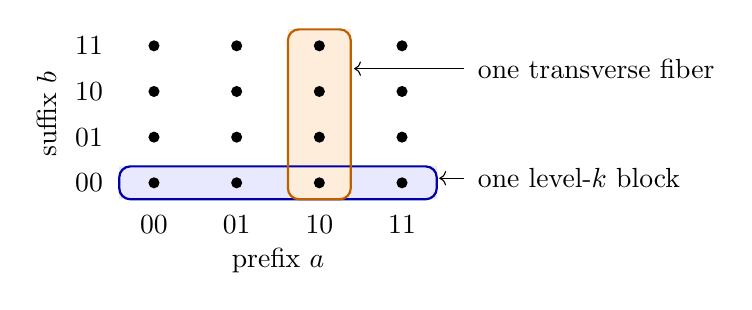
\begin{tikzpicture}[x=1.05cm,y=.58cm]
 \fill[blue!9] (-.42,-.36) rectangle (3.42,.36);
 \fill[orange!14] (1.62,-.36) rectangle (2.38,3.36);
 \draw[blue!65!black,thick,rounded corners] (-.42,-.36) rectangle (3.42,.36);
 \draw[orange!75!black,thick,rounded corners] (1.62,-.36) rectangle (2.38,3.36);
 \foreach \x in {0,1,2,3} {
   \foreach \y in {0,1,2,3} {\fill (\x,\y) circle (2pt);}
 }
 \node[below] at (0,-.5) {$00$};
 \node[below] at (1,-.5) {$01$};
 \node[below] at (2,-.5) {$10$};
 \node[below] at (3,-.5) {$11$};
 \node[left] at (-.5,0) {$00$};
 \node[left] at (-.5,1) {$01$};
 \node[left] at (-.5,2) {$10$};
 \node[left] at (-.5,3) {$11$};
 \node at (1.5,-1.7) {prefix $a$};
 \node[rotate=90] at (-1.3,1.5) {suffix $b$};
 \node[right,align=left] at (3.8,.1) {one level-$k$ block};
 \node[right,align=left] at (3.8,2.5) {one transverse fiber};
 \draw[->] (3.75,.1)--(3.45,.1);
 \draw[->] (3.75,2.5)--(2.42,2.5);
\end{tikzpicture}
\caption{The case $d=4$, $k=2$. The first $k$ layers act within
the horizontal blocks. After those layers are fixed, the remaining
layers evolve independently in the vertical fibers. Each horizontal
block receives one final site from every fiber.}
\label{cycles:transverse-figure}
\end{figure}

\begin{lemma}[Statistics after one sweep]\label{sweeps:block-statistics}
Fix $0<\varepsilon\le1$. Start a sweep from deterministic $(F,f)$
with $|F|\ge\varepsilon n$, $\sum_xf(x)=0$, and energy
$E_0=\|f\|_2^2$. Denote its output by $(F^*,f^*)$ and write
$S_B=\sum_{x\in B}f^*(x)$ and $m_B=|F^*\cap B|$. For
$B\in\mathcal B_j$, of size $s=2^j$,
\begin{equation}\label{sweeps:block-variance}
 \E S_B^2\le(s/n)E_0,\qquad
 \Pr(m_B<\varepsilon s/2)\le e^{-\varepsilon^2s/2}.
\end{equation}
The second bound can alternatively be replaced by
$\exp[-(1/2-e^{-1})\varepsilon s]$.
\end{lemma}
\begin{proof}
Condition on the configuration after coordinate $j$. The remaining
layers use independent switch arrays in the $s$ transverse fibers,
each of size $n/s$. The final entry at the one site where a fiber
meets $B$ has conditional mean equal to that fiber's mean signed
weight and second moment at most its mean squared weight, by
\eqref{cycles:mean-update}. The sum of these means is
$(s/n)\sum_x f(x)=0$. Independence between fibers therefore bounds
the conditional second moment of $S_B$ by $(s/n)$ times the energy
at the conditioning time, which is at most $E_0$.

The availability indicators at those $s$ sites are likewise independent
under this conditioning. Their total mean is
$\mu=|F|s/n\ge\varepsilon s$. Hoeffding's inequality
(Lemma~\ref{lem:concentration}) bounds a downward deviation of at least
$\varepsilon s/2$ by $e^{-\varepsilon^2s/2}$. Alternatively, for their
sum $J$, independence gives
$\E e^{-J}\le e^{-(1-e^{-1})\mu}$, and hence
$\Pr(J<\mu/2)\le e^{-(1/2-e^{-1})\mu}$.
\end{proof}

The next identity describes how a sweep uses these block statistics.
Its inputs are deterministic at the start of that sweep; no independence
between blocks of a preceding sweep's output is required.

\begin{lemma}[The block-merging identity]\label{sweeps:merge}
Start a sweep deterministically. Suppose two sibling blocks have size
$s$, available counts $m_0,m_1$ and signed sums $S_0,S_1$. Let
$\overline E_0,\overline E_1$ be their expected energies after their
internal coordinates have been updated. The expected energy after
their merging coordinate is
\begin{equation}\label{sweeps:merge-eq}
 (1-m_1/(2s))\overline E_0+
 (1-m_0/(2s))\overline E_1+S_0S_1/s.
\end{equation}
\end{lemma}
\begin{proof}
The child blocks use independent switch arrays before merging.
The averaging identities in \eqref{cycles:mean-update} give, at each
site of child $i$, expected availability $m_i/s$ and expected signed
weight $S_i/s$. No equality between the individual sites' second
moments is needed. On an edge with weights $a,b$ and availability
indicators $q_a,q_b$, the energy loss is
$(q_ba^2+q_ab^2-2ab)/2$. Independence across children and summation
over their $s$ paired sites give expected loss
\[
 \frac{m_1\overline E_0+m_0\overline E_1-2S_0S_1}{2s},
\]
which proves the identity.
\end{proof}

\subsection{Transverse block sampling and zero block sums}
\label{cycles:zero-block}

The next argument first removes the small component that is constant on
the available positions of each block. The remaining component has zero expected
weight at each site in the latter half of the next sweep.

\begin{proposition}[Blockwise centered contraction]
\label{cycles:centered-prop}
For $p=1/16$, arbitrary $|F|\ge pn$, and zero-sum $f$, two sweeps
satisfy \eqref{cycles:coarse-contraction}. After $2048$ sweeps every
fixed list of at most $15n/16$ labels has variation error at most
$\frac12 n^{-1/2}$.
\end{proposition}
\begin{proof}
Put $k=\lfloor d/2\rfloor$, $L=2^k$, and $M=2^{d-k}$, and denote
the first-sweep output by $(F^*,f^*)$. Sum the moment bound in
Lemma~\ref{sweeps:block-statistics} over the $M$ level-$k$ blocks.
Its exponential tail, using $1/2-e^{-1}>1/8$, and a union bound give
\begin{equation}\label{cycles:transverse}
 \Pr(\mathcal G^c)\le M e^{-pL/8},\qquad
 \E\sum_B S_B^2\le\|f_0\|_2^2,\qquad
 \mathcal G=\{|F^*\cap B|\ge pL/2\text{ for every }B\}.
\end{equation}
For each first-sweep output in $\mathcal G$, write $f^*=u+w$, where
$u$ has constant value $S_B/|F^*\cap B|$ on each $F^*\cap B$.
This is an orthogonal decomposition, $w$ has zero sum in each block, and
\[
 \|u\|_2^2=\sum_B\frac{S_B^2}{|F^*\cap B|}
       \le\frac{2}{pL}\sum_BS_B^2.
\]
Run $w$ through the second sweep. After the first $j\ge k$ coordinates,
its expected value at each site is zero and the probability of availability is at
least $p/2$. Different level-$j$ blocks have evolved independently, so
at the next merging pair the expected product of weights is zero.
In the energy-loss formula the opposite flag multiplies each squared
weight independently, with expectation at least $p/2$. The expected
energy hence contracts by $1-p/4$ for each of the last $d-k$ layers.
The $u$ component cannot increase in norm. Using
$\|u_{\rm out}+w_{\rm out}\|_2^2\le2\|u_{\rm out}\|_2^2+
2\|w_{\rm out}\|_2^2$, and monotonicity outside $\mathcal G$, proves
\begin{equation}\label{cycles:centered-factor}
 \E\|f_{2d}\|_2^2\le
 \left(Me^{-pL/8}+2(1-p/4)^{d-k}+\frac4{pL}\right)\|f_0\|_2^2.
\end{equation}
Here $(1-p/4)^{d-k}\le e^{-d/128}$, and the other terms decay faster
than $n^{-1/256}$. Thus their sum is at most $n^{-1/256}$ eventually.
After $1024$ two-sweep blocks the energy is at most $n^{-4}$;
Lemma~\ref{cycles:list} proves the conclusion.
\end{proof}

\subsection{A recurrence for all large blocks}
\label{cycles:merge}

One can retain the block sums in the recurrence instead of separating
them off. This yields a useful contraction for every fixed density of available positions.

\begin{proposition}[Multilevel energy contraction]
\label{cycles:merge-prop}
Fix $p\in(0,1)$ and set $r=\lfloor d/2\rfloor$. For arbitrary
$|F|\ge pn$ and zero-sum $f$, two sweeps satisfy
\begin{equation}\label{cycles:merge-factor}
 \E\|f_{2d}\|_2^2\le
 \left((1-p/4)^{d-r}+2^{-r}
             +2^{d-r}e^{-p2^r/8}\right)\|f_0\|_2^2.
\end{equation}
In particular the factor is at most $n^{-\gamma_p}$ eventually, where
$\gamma_p=-\frac14\log_2(1-p/4)>0$.
It is also at most $n^{-p/16}$ eventually.
\end{proposition}
\begin{proof}
For level-$i$ blocks $B$ of size $2^i$, define
\[
 S_i(f)=2^{-i}\sum_B\left(\sum_{x\in B}f(x)\right)^2.
\]
The block statistics of Lemma~\ref{sweeps:block-statistics}, now
applied at every level $i$, give
\begin{equation}\label{cycles:all-level-moments}
 \E S_i(f^*)\le2^{-i}\|f_0\|_2^2,\qquad
 \Pr\{\text{some level-$r$ block has density below }p/2\}
 \le2^{d-r}e^{-p2^r/8}.
\end{equation}
Indeed each level-$i$ block meets every transverse fiber once.
Lemma~\ref{sweeps:block-statistics}, summed over the $n/2^i$ blocks,
gives the first bound. For the second, its proof gives a sum of independent
availability indicators of mean at least $p2^r$; the Bernoulli lower-tail
bound used in \eqref{cycles:transverse} and a union bound suffice.

Condition now on $f^*,F^*$ with all level-$r$ block densities at
least $p/2$. Their unions have the same lower density bound. In the
second sweep, Lemma~\ref{sweeps:merge} therefore multiplies each
child energy by at most $1-p/4$. Its signed cross term is bounded
using $2S_{B_0}S_{B_1}\le S_{B_0}^2+S_{B_1}^2$. Summing over
merges of level-$i$ blocks, and writing $E_i$ for the energy after
$i$ layers of this sweep, gives
\[
 \E(E_{i+1}\mid f^*,F^*)
 \le(1-p/4)\E(E_i\mid f^*,F^*)+\frac12S_i(f^*),
 \qquad r\le i<d.
\]
Iterate, discard the contraction factors on the nonnegative additive
terms, use \eqref{cycles:all-level-moments}, and use pathwise monotonicity
on the excluded event. The geometric sum
$\frac12\sum_{i=r}^{d-1}2^{-i}\le2^{-r}$ proves
\eqref{cycles:merge-factor}. Its first term is at most $n^{-2\gamma_p}$;
the other terms are $O(n^{-1/2})$ and exponentially small in $\sqrt n$,
respectively. Since $\gamma_p<1/2$, their sum is at most
$n^{-\gamma_p}$ eventually. Also the first term is at most
$e^{-pd/8}=n^{-p/(8\log2)}$, whose exponent exceeds $p/16$,
proving the alternative assertion.
\end{proof}

\begin{remark}[Translation symmetry and a variant of the error bound]
\label{cycles:invariance}
A completed block also has a distributional symmetry. After its $i$
internal coordinates have been processed, its flag-weight law is
invariant under bit translations of those coordinates. Inductively,
old-coordinate translations permute the fresh matching edges, while
flipping the new coordinate preserves the independent fair placements
and the equal outputs of averaging. The symmetry makes each site's
second moment the expected block energy divided by $2^i$.

This supplies another derivation of \eqref{sweeps:merge-eq}, although
the first-moment proof of Lemma~\ref{sweeps:merge} does not require it.
It also permits the following version of the multilevel estimate.
For the first-sweep output,
$\E\sum_{B\in\mathcal B_i}S_B^2\le\|f_0\|_2^2$ and
$\Pr(m_B<p2^i/2)\le e^{-p2^i/8}$. A union bound over every level
$r\le i<d$, followed by the exact merge identity and
$2S_{B_0}S_{B_1}\le S_{B_0}^2+S_{B_1}^2$, gives
\begin{equation}\label{cycles:invariance-factor}
 (1-p/4)^{d-r}+2^{-r}+dn e^{-p2^r/8}\le n^{-p/16}
\end{equation}
for large $d$. This is a slightly weaker error term than
\eqref{cycles:merge-factor}; both bounds condition on the full
first-sweep output before using fresh, independent second-sweep blocks.
\end{remark}

\subsection{Negative correlation and block variances}
\label{cycles:negative}

The last two-sweep argument obtains first-sweep moments from pairwise
negative correlation of card locations. It then contracts variance
about the mean on the available positions of each block.

\begin{proposition}[Variance contraction from pairwise correlation]
\label{cycles:negative-prop}
Fix $\delta\in(0,1]$. For arbitrary $|F|\ge\delta n$ and zero-sum $f$,
there is $a=a(\delta)>0$ such that two sweeps satisfy
$\E\|f_{2d}\|_2^2\le n^{-a}\|f_0\|_2^2$ for all large $d$.
One may take $a=-\frac18\log_2(1-\delta/4)$.
\end{proposition}
\begin{proof}
For a level-$s$ block $B$ put $p_B=|B|/n$. Membership in $B$
means that the last $d-s$ output bits equal its prescribed suffix.
Every card has membership probability $p_B$. To compare two distinct
cards, let $i$ be their largest initially differing coordinate. Before
layer $i$, they use distinct switches, so their output bits are
independent fair bits. At layer $i$ they use one switch exactly when
their earlier output prefixes agree; that switch forces opposite
outputs. After layer $i$ their prefixes are distinct, and they use
distinct switches for the rest of the sweep.

If $i\le s$, the only possible shared switch is in an unconstrained
coordinate. All prescribed suffix bits are then sampled at distinct
switches, and joint membership has probability $p_B^2$. If $i>s$,
condition on both cards having the prescribed outputs at coordinates
$s+1,\ldots,i-1$. Their first $s$ outputs remain independent uniform
strings, so their prefixes agree with probability $2^{-s}$. On this
event joint membership is impossible at layer $i$; off it both
prescribed outputs occur with probability $1/4$. The remaining
prescribed bits are again sampled at distinct switches. Thus joint
membership has probability $p_B^2(1-2^{-s})\le p_B^2$.
In either case the membership indicators have nonpositive covariance.

Let $C$ be the covariance matrix of the membership indicators of all $n$
initial labels. Their sum is the fixed number $|B|$, so $C$ has zero row
sums. Its off-diagonal entries are nonpositive, and its diagonal is at
most $p_B$. Therefore
\[
 v^TCv=\sum_{x<y}(-C_{xy})(v_x-v_y)^2
 \le2p_B\sum_xv_x^2.
\]
Let $h_B$ count the cards that start in $F_0$ and end in $B$, and let
$u_B$ be the sum of averaged loads there. It follows that
\begin{equation}\label{cycles:negative-moments}
 \E h_B=p_B|F|,\qquad
 \operatorname{Var}(h_B)\le p_B|F|,\qquad
 \E u_B^2\le2p_B\|f_0\|_2^2.
\end{equation}
For the last estimate, give the card initially at $a\in F_0$ the
deterministic signed weight $f_0(a)$, and give every observed card,
initially outside $F_0$, weight zero. If $g_t$ is the actual position
permutation, the transported load is
$\widetilde f_t(x)=f_0(g_t^{-1}x)$, with $f_0$ extended by zero.
Fix a feasible history $\mathcal H$ of all observed-card trajectories
through the first sweep. Lemma~\ref{lem:marginal-averaging} leaves the
unvisited switches independent and fair, including an earlier unvisited
switch when later observed paths are specified. The additional step here
is to apply that conditional-flow rule to arbitrary signed loads.
At a pair with two available inputs, averaging that unvisited fair coin
averages the two incoming expected loads. At a pair with one available input,
the observed trajectory determines its available output, so its load is
transported to that output. Induction over layers, using linearity for
the signed weights, therefore gives
\begin{equation}\label{cycles:signed-load-jensen}
 f_t(x)=\E[\widetilde f_t(x)\mid\mathcal H],\qquad
 u_B=\E\!\left[\sum_{a\in F_0}f_0(a)
                    \mathbf1_{\{g_d(a)\in B\}}\,
                    \middle|\,\mathcal H\right].
\end{equation}
Each initial label has probability $p_B$ of ending in $B$, and
$\sum_a f_0(a)=0$, so the unaveraged sum has mean zero and second moment
$f_0^TCf_0\le2p_B\|f_0\|_2^2$. Conditional Jensen proves the asserted
bound for $u_B$ for every signed initial load.

If $\delta=1$, every position is available, so one sweep applies all
coordinate averages and sends the zero-sum vector to zero. The list
statement then concerns the empty list and is exact. For the remaining
argument assume $0<\delta<1$.

Put $s_0=\lfloor3d/4\rfloor$. Chebyshev gives probability at most
$4/(\delta2^s)$ that a fixed level-$s$ block has
$h_B<\delta2^s/2$. There are $n/2^s$ such blocks. Summing over
$s\ge s_0$ bounds the failure probability by
$O_\delta(n2^{-2s_0})=O_\delta(n^{-1/2})$.
Condition on a first-sweep output outside that event. At a second-sweep
merge of children $L,R$ of size $m=2^{s-1}$, write
$b_L=u_L/h_L$, $b_R=u_R/h_R$ for their means over available positions.
Let $V_L,V_R$ be their expected squared deviations from these means
immediately before the merge, and $V_B$ the corresponding parent
quantity. Subtracting the parent mean energy from the common
block-merging identity, Lemma~\ref{sweeps:merge}, gives
\begin{align}\label{cycles:variance-merge}
 V_B={}&\left(1-\frac{h_R}{2m}\right)V_L+
 \left(1-\frac{h_L}{2m}\right)V_R\notag\\
 &+\left(1-\frac{h_L+h_R}{2m}\right)
       \frac{h_Lh_R}{h_L+h_R}(b_L-b_R)^2.
\end{align}
To verify it, the premerge total energy is
$V_L+V_R+h_Lb_L^2+h_Rb_R^2$; the expected loss is
$[h_RV_L+h_LV_R+h_Lh_R(b_L-b_R)^2]/(2m)$.
Subtract the parent mean term
$(h_Lb_L+h_Rb_R)^2/(h_L+h_R)$ to obtain the formula.
All denominators are positive on the retained event.

For $s>s_0$ the first two coefficients are at most $1-\delta/4$.
The last term is nonnegative and at most
$u_L^2/h_L+u_R^2/h_R$. Iterating to the root, whose load mean is zero,
bounds the final conditional energy by
\[
 (1-\delta/4)^{d-s_0}\|f_0\|_2^2+
 \sum_{s=s_0}^{d-1}\frac{2}{\delta2^s}
                   \sum_{|B|=2^s}u_B^2.
\]
For each level \eqref{cycles:negative-moments} bounds the expectation
of the inner sum by $2\|f_0\|_2^2$. Use monotonicity on the discarded
event. The resulting two-sweep factor is
\begin{equation}\label{cycles:negative-factor}
 (1-\delta/4)^{d-s_0}
       +O_\delta(2^{-s_0})+O_\delta(n2^{-2s_0}).
\end{equation}
Its leading term is at most $n^{-2a}$ for the stated $a$, and the two
other terms are $O_\delta(n^{-3/4})$ and $O_\delta(n^{-1/2})$.
This proves the claim. By Lemma~\ref{cycles:list}, any fixed
$R$ with $aR>3$ now suffices for the asserted large-list mixing.
\end{proof}

\subsection{From the two-sweep estimates to the full deck}
\label{cycles:two-sweep-completion}

The five energy estimates give different quantitative parameters for the
abstract Fourier transfers, even when two total times coincide. We record the exact
substitutions. For disjoint block subgroups $H_i=\Sym(D_i)$, a
subprobability $\nu$ satisfying $\nu(gH_i)\le B/[G:H_i]$ has
\begin{equation}\label{cycles:orbit-bound}
 \|\widehat\nu(\rho)\|_{\op}
 \le\sqrt{rBC_s}\,D^{-(1-(s+2)/r)/2},
\end{equation}
by Proposition~\ref*{l-l:orbit-span} of \cite{partialFourier}. Here $r$ is the
number of blocks, $D=\dim\rho$, and $C_s$ is the reciprocal-degree
constant defined in Section~\ref{mart:applications}. That companion
also proves two distinct central-projection bounds in
Proposition~\ref*{l-l:central-projector-operator} of~\cite{partialFourier}. For a probability
$\eta$ with the same caps they are
\begin{align}
 \|\widehat\eta(\rho)\|_{\op}
 &\le BC_s\sqrt r\,D^{-1/2+(s+2)/r},\label{cycles:projector-op-one}\\
 \|\widehat\eta(\rho)\|_{\op}
 &\le B\sqrt{rC_s}\,D^{-1/2+(s+2)/(2r)}.\label{cycles:projector-op-two}
\end{align}
The first uses pointwise character control; the second uses cosetwise
spectral projection. Both require one simultaneous cap for all the
subgroups. Lemma~\ref*{l-l:trim} of~\cite{partialFourier} supplies it with the mass costs stated
in Section~\ref{mart:applications}.

\begin{proposition}[Full-deck bounds from two sweeps]
\label{cycles:two-sweep-bounds}
Each row of Table~\ref{cycles:transfer-table} gives total-variation
convergence of the full permutation law to uniform as $d\to\infty$,
uniformly over deterministic initial decks.
\end{proposition}

In the table, $r$ counts equal label blocks, $T$ is the length of one
shuffle block, and $\ell$ counts independent shuffle blocks. For the
multilevel row set
\[
 \gamma=-\tfrac14\log_2(127/128),\qquad h=\lceil6/\gamma\rceil.
\]
In the translation row use $R=128\cdot128$. In the negative-correlation
row, $R$ is any fixed integer with $a(1/8)R>3$, where $a$ is from
Proposition~\ref{cycles:negative-prop}. Each displayed Fourier bound is
an operator-norm bound at irreducible degree $D$.

\begingroup
\small
\setlength{\tabcolsep}{4pt}
\renewcommand{\arraystretch}{1.2}
\begin{longtable}{@{}p{.32\linewidth}p{.31\linewidth}r r r@{}}
\caption{Two-sweep inputs and their full-deck substitutions.
The exponent $\kappa$ is $2-2\ell\alpha$ for an operator bound
$K D^{-\alpha}$.}\label{cycles:transfer-table}\\
\toprule
Input and retained measure & Transfer and Fourier bound
 & $\ell$ & $\kappa$ & Total time$/d$\\
\midrule
\endfirsthead
\toprule
Input and retained measure & Transfer and Fourier bound
 & $\ell$ & $\kappa$ & Total time$/d$\\
\midrule
\endhead
\bottomrule
\endfoot
Coarse energy, $T/d=4096$;\newline
$r=8$, probability, cap $2$
&
Orbit, \eqref{cycles:orbit-bound}, $s=1$;\newline
$\sqrt{16C_1}D^{-5/16}$
& $8$ & $-3$ & $32768$\\
Blockwise centered, $T/d=2048$;\newline
$r=16$, subprobability, cap $1$
&
Orbit, \eqref{cycles:orbit-bound}, $s=4$;\newline
$\sqrt{16C_4}D^{-5/16}$
& $16$ & $-8$ & $32768$\\
Multilevel, $p=1/32$, $T/d=2h$;\newline
$r=32$, cap-one subprobability,\newline
then restore uniform mass
&
Orbit, \eqref{cycles:orbit-bound}, $s=8$;\newline
$\sqrt{32C_8}D^{-11/32}$
& $16$ & $-9$ & $32h$\\
Translation symmetry, $p=1/128$,\newline
$T/d=2R$; $r=128$,\newline
probability, cap $4$
&
Pointwise projector,\newline
\eqref{cycles:projector-op-one}, $s=6$;\newline
$4C_6\sqrt{128}D^{-7/16}$
& $16$ & $-12$ & $524288$\\
Negative correlation, $\delta=1/8$,\newline
$T/d=2R$; $r=8$,\newline
probability, cap $3$
&
Cosetwise projector,\newline
\eqref{cycles:projector-op-two}, $s=2$;\newline
$3\sqrt{8C_2}D^{-1/4}$
& $8$ & $-2$ & $16R$\\
\end{longtable}
\endgroup

\begin{proof}
The input marginal errors follow from Lemma~\ref{cycles:list}.
The coarse and centered bounds are those of
Propositions~\ref{cycles:coarse-prop} and \ref{cycles:centered-prop}.
For the multilevel row, Proposition~\ref{cycles:merge-prop} gives
energy $n^{-h\gamma}$ and marginal error
$\varepsilon_n\le\tfrac12n^{(3-h\gamma)/2}=o(1)$.
For translation symmetry, \eqref{cycles:invariance-factor} has exponent
$p/16=1/2048$, so $(p/16)R=8$ and the marginal error is
$\tfrac12n^{-5/2}$. The last row has error
$\tfrac12n^{(3-a(1/8)R)/2}=o(1)$.
Each bound is uniform, so any fixed partition into the indicated
$r$ equal blocks supplies all the complementary marginals.

Use the simultaneous trimming operations of
Section~\ref{mart:applications}. For the first row, excess trimming
followed by normalization gives cap $2$ eventually. For the fourth
and fifth, heavy-coset deletion and normalization give caps $4$ and
$3$. These probability laws are within $o(1)$ of their original block
laws. The second and third rows retain cap-one subprobabilities before
their different completions.

Substituting the table's caps, block counts and reciprocal-degree
parameters in the preceding three transfer formulas gives its Fourier
bounds. The exponents $\kappa$ follow from
$D\|M^\ell\|_{\HS}^2\le D^2\|M\|_{\op}^{2\ell}$.
Their sums tend to zero by the respective reciprocal-degree estimates
at powers $1,4,8,6,2$ in
\cite[Theorem~\ref*{l-l:degree-all-powers}]{partialFourier}.

For the multilevel row, the cap-one construction loses mass
$\delta\le32\varepsilon_n$. Restore it as $\eta=\nu+\delta U_G$.
Every nontrivial Fourier matrix of $\eta$ equals that of $\nu$, so
the table's orbit bound still applies, and
$\|\eta-\mu\|_{\TV}\le\delta=o(1)$ for the original block law $\mu$.
Thus this row, like the first, fourth and fifth, meets the probability
completion of Section~\ref{sec:probability-completion}: the original
law has zero sign expectation, the nearby probability has sign
coefficient $o(1)$, and replacing the fixed number of factors costs
$o(1)$.

The centered row instead convolves the cap-one subprobability itself.
Write $z=\nu(G)\to1$. Domination by the original unbiased-sign block
law gives $|\widehat\nu(\sgn)|\le1-z$. Its nonsign contribution is
bounded by $(16C_4)^{16}\sum_{D>1}D^{-8}=o(1)$.
Equation~\eqref{noise:subprob-plancherel} therefore gives
$\|\nu^{*16}-z^{16}U_G\|_1=o(1)$. The positive difference
$\mu^{*16}-\nu^{*16}$ has mass $1-z^{16}\le16(1-z)=o(1)$,
which restores the original probability law.

Finally each block contains a whole number of sweeps, so the physical
time is $\ell T$, as tabulated. Translation by a deterministic initial
deck preserves the distance from uniform.
\end{proof}

\section{Autocorrelation and two independent shuffle blocks}
\label{cycles:autocorrelation-section}

Keeping the bitwise difference of two factors of the conditional weight
gives another derivation of the scalar energy recurrence. For the final passage to the
full group, we will use one measure capped on $gH_i$ and a second measure
capped on $H_ig$. Reversing the coordinate schedule supplies the second
measure; the original block law itself need not be invariant under
inversion.

Let $q_d$ be the probability law on $G$ of one physical shuffle.

\begin{theorem}[Two-block cyclic-schedule bound]
\label{cycles:sharp}
For the Thorp shuffle on $n=2^d$ positions,
\[
 \|q_d^{*2052d}-U_G\|_{\TV}\longrightarrow0
 \qquad(d\longrightarrow\infty).
\]
In particular $d\le t_{\mathrm{mix}}(d)\le2052d$ for all sufficiently
large $d$.
\end{theorem}

\subsection{The bitwise autocorrelation recurrence}
\label{cycles:autocorrelation}

Fix an ordered list of $q\le7n/8$ initial labels, observe the first
$j<q$ cards, and use the centered conditional vector $f_t$ from
\eqref{cycles:conditional-weight}. Write $O_t=V\setminus F_t$ and
$h(t)$ for the coordinate used from time $t$ to time $t+1$.
The schedule $h(t)$ can be any periodic ordering of all coordinates.
Define
\begin{equation}\label{cycles:autocorrelation-definition}
 r_t=\E\|f_t\|_2^2,\qquad
 v_t(z)=\E\sum_{x\in V}f_t(x)f_t(x\oplus z),\qquad
 b_t=\E\sum_xf_t(x)^2\one_{\{x\oplus e_{h(t)}\in O_t\}}.
\end{equation}
Here $\oplus$ is bitwise addition and $e_h$ is the unit bit vector.
The signed row $v_t$ has total mass zero, since $\sum_xf_t(x)=0$,
and $v_t(0)=r_t$. Let $L_h$ replace coordinate $h$ by an independent
fair bit, as a kernel on the difference variable $z$.

\begin{lemma}[Finite-memory identity]
\label{cycles:memory}
For every $t\ge0$,
\begin{equation}\label{cycles:autocorrelation-update}
 v_{t+1}=v_tL_{h(t)}+\frac12b_t(\delta_0-\delta_{e_{h(t)}}).
\end{equation}
Consequently, for $t\ge d$,
\begin{equation}\label{cycles:memory-equation}
 r_t=\sum_{\ell=1}^d2^{-\ell}b_{t-\ell}.
\end{equation}
\end{lemma}
\begin{proof}
Condition on the observed paths through $t$. Let $K_t$ be the random
kernel from the old available set to the new one: its rows are uniform on
pairs with two available endpoints and deterministic at a single available endpoint, with
its destination specified by the fresh observed movement. Expand the
autocorrelation of $f_tK_t$. This is a sum over two available starting
endpoints $x,y$, weighted by $f_t(x)f_t(y)$, of the law of the difference
of two independent draws from their rows, conditional on $K_t$.
For endpoints in distinct pairs, their fresh pair data are independent;
after averaging the fresh coins, their difference has kernel $L_{h(t)}$.
For two endpoints in the same pair with two available inputs, including
$x=y$, the two row draws are independent uniform draws, so the same
conclusion holds.
The only exception is $x=y$ with its partner observed. Both row draws
then equal the same deterministic destination. Their difference is zero
rather than the fair choice between $0$ and $e_{h(t)}$.
Summing these corrections gives \eqref{cycles:autocorrelation-update}.

The product of all $d$ coordinate-reset kernels maps a signed row to
its total mass times uniform; it therefore kills $v_{t-d}$.
A correction created at step $s$, $t-d\le s<t$, has not yet had its
own coordinate reset again. Subsequent resets transfer a fraction
$2^{-(t-1-s)}$ of $\delta_0$ to zero, and transfer none of
$\delta_{e_{h(s)}}$ to zero. Including the prefactor $1/2$ and summing
all $d$ corrections gives \eqref{cycles:memory-equation}.
\end{proof}

\begin{lemma}[Opposite-half control]
\label{cycles:halves}
Put $\theta=15/16$ and $\epsilon_n=2e^{-n/256}$. For $s\ge d$,
\begin{equation}\label{cycles:blocked-bound}
 b_s\le\theta r_s+\epsilon_n.
\end{equation}
With $\gamma=63/64$, it follows that
\begin{equation}\label{cycles:autocorrelation-energy}
 r_t\le\gamma^{t-2d}+\frac{\epsilon_n}{1-\theta}
 \quad(t\ge2d),\qquad
 r_{1026d}\le2n^{-16}
\end{equation}
for all sufficiently large $d$.
\end{lemma}
\begin{proof}
The autocorrelation notation has $r_t=a_t$ and $b_t=w_t$ from
Section~\ref{sec:first-route}. There are at most $7n/8$ blockers,
so Lemma~\ref{noise:halves} with $\alpha=1/8$ gives
\eqref{cycles:blocked-bound}. Its independence step is the exact
opposite-half identity
\begin{equation}\label{cycles:half-factorization}
 \E\!\left[\sum_{x\in H_0}f_s(x)^2
       \one_{\{x\oplus e_{h(s)}\in O_s\}}
       \,\middle|\,\mathcal F_{s-d+1}\right]
 =\frac{|O_{s-d+1}\cap H_1|}{n/2}
       \E\!\left[\sum_{x\in H_0}f_s(x)^2
       \,\middle|\,\mathcal F_{s-d+1}\right],
\end{equation}
where $H_0,H_1$ are the two coordinate-$h(s)$ halves. The conditioning
time is just after that coordinate's preceding update; only the
subsequent independent arrays in the two halves are averaged here.

Insert \eqref{cycles:blocked-bound} into the autocorrelation memory
identity. The comparison \eqref{noise:comparison-solution} applies with
$\rho=\theta$, $\eta=\epsilon_n$, $t_0=2d$, and $\gamma=63/64$,
since $\theta/(2\gamma-1)=30/31<1$. This proves the first energy bound.
At $t=1026d$, $\gamma^{1024d}\le e^{-16d}\le n^{-16}$, and
$\epsilon_n/(1-\theta)\le n^{-16}$ eventually, giving the last bound.
\end{proof}

\subsection{Pointwise bounds with a predictable discard}
\label{cycles:predictable}

Expected total variation sufficed for the preceding proofs. For two
blocks it is useful to retain a pointwise cap on a large subprobability.
The discard must be made through events measurable from preceding paths.

\begin{lemma}[Subprobability bound for a prescribed list]
\label{cycles:list-cap}
Let $T=1026d$ and let the coordinate order be any periodic permutation
of $1,\ldots,d$. For all sufficiently large $d$ and every fixed list
$a_1,\ldots,a_q$ with $q\le7n/8$, there is an event $E$ with
$\Pr(E^c)\le2n^{-9}$ such that for every
ordered distinct target tuple $(y_1,\ldots,y_q)$,
\begin{equation}\label{cycles:pointwise-list}
 \Pr(E,\ X_T(a_i)=y_i\ (1\le i\le q))
 \le\frac{(1+n^{-2})^q}{(n)_q},
 \qquad (n)_q=n(n-1)\cdots(n-q+1).
\end{equation}
\end{lemma}
\begin{proof}
For each $0\le j<q$, construct $f_T^{(j)}$ by observing the first $j$
paths and centering the conditional law of card $j+1$.
Let $E_j=\{\max_x|f_T^{(j)}(x)|\le n^{-3}\}$, an event measurable
from those $j$ paths. The energy bound and Markov's inequality give
$\Pr(E_j^c)\le2n^{-10}$. Take $E=\bigcap_{j<q}E_j$.

To bound the probability for the first $j+1$ targets and events
$E_0,\ldots,E_j$, condition on the first $j$ trajectories. The preceding
target constraints and those events are measurable there. On $E_j$ the
next target has conditional probability at most
\[
 \frac1{n-j}+n^{-3}\le\frac{1+n^{-2}}{n-j}.
\]
After applying this upper bound, drop $E_j$ and repeat for the preceding
$ j$ targets and events. Induction gives \eqref{cycles:pointwise-list}.
This argument retains subprobabilities throughout; it never asserts
that the one-card estimates survive conditioning on the entire event $E$.
\end{proof}

\begin{lemma}[Separate bounds for multiplication on each side]
\label{cycles:two-sided-cap}
Let $\mu=q_d^{*T}$, $T=1026d$, and partition $V$ into eight sets
$D_i$ of size $n/8$, with $H_i=\Sym(D_i)$ fixing the complement.
There are subprobabilities $\alpha,\beta\le\mu$, each of mass
$1-O(n^{-9})$, whose densities $A,B$ with respect to uniform measure
on $G$ satisfy
\begin{equation}\label{cycles:two-sided-density}
 \int_{H_i} A(h^{-1}g)\,dh\le2,
 \qquad
 \int_{H_i} B(gh^{-1})\,dh\le2
 \quad(g\in G,\ 1\le i\le8).
\end{equation}
All subgroup integrals use normalized counting measure.
\end{lemma}
\begin{proof}
For each $i$ take a fixed ordered list of the complement of $D_i$ and
apply Lemma~\ref{cycles:list-cap} in the same forward shuffle space.
Intersect the eight retained events and let $\beta$ be the law of the
endpoint permutation on this intersection. Its lost mass is at most
$16n^{-9}$. The image constraints are the coset $gH_i$, so inclusion
and \eqref{cycles:pointwise-list} give
\[
 \beta(gH_i)\le\frac{(1+n^{-2})^{7n/8}}{[G:H_i]}.
\]
Since $(1+n^{-2})^{7n/8}\le2$ for large $n$, this is the second cap.

For the first cap, use the law of the inverse permutation. A physical
$T$-step block is a product of complete cyclic coordinate sweeps with
no residual rotation. Every matching layer is an involution, and all
layers are independent; hence its inverse law is generated by the same
layers in reverse order. The reversed order is again a periodic
coordinate schedule, to which Lemma~\ref{cycles:list-cap} applies.
Intersect its eight events, producing a subprobability
$\widetilde\alpha\le\mathcal L(g^{-1}:g\sim\mu)$, then push it
forward under inversion to obtain $\alpha\le\mu$.
The image constraint for $g^{-1}$ becomes the preimage constraint for
$g$, whose fiber is $H_ig$. Consequently
$\alpha(H_ig)\le2/[G:H_i]$, the first cap.
To check the density normalization explicitly,
\[
 \int_{H_i}A(h^{-1}g)\,dh=[G:H_i]\alpha(H_ig),\qquad
 \int_{H_i}B(gh^{-1})\,dh=[G:H_i]\beta(gH_i).
\]
Thus the two laws may differ, but each is dominated by the same physical
block law, on the required side of multiplication.
\end{proof}

\subsection{Completing the two-block argument}
\label{cycles:two-block-completion}

The remaining step uses precisely the opposite-side caps just proved.
For a density $A$ relative to $U_G$, write
$\widehat A(\rho)=\int_G A(g)\rho(g)\,dU_G(g)$, so if $A$ is the
density of $\alpha$ this is exactly the mass transform
$\widehat\alpha(\rho)$. Use the same convention for $B$ and $\beta$.
Density convolution is
$B*A(g)=\int_G B(h)A(h^{-1}g)\,dU_G(h)$; thus
$\widehat{B*A}(\rho)=\widehat B(\rho)\widehat A(\rho)$.
The two-sided transfer, Theorem~\ref*{l-l:two-sided} of
\cite{partialFourier}, applies to the two nonnegative densities of mass
at most one because Lemma~\ref{cycles:two-sided-cap} gives
\[
 \int_{H_i}A(h^{-1}g)\,dh\le2,\qquad
 \int_{H_i}B(gh^{-1})\,dh\le2
 \quad(g\in G,\ 1\le i\le8).
\]
Its conclusion is
\begin{equation}\label{cycles:two-sided-fourier-bound}
 D_\lambda\|\widehat B(\lambda)\widehat A(\lambda)\|_{\HS}^2
 \le4K_\lambda^2D_\lambda^{-1/2}.
\end{equation}
Here $D_\lambda$ is the irreducible dimension and $K_\lambda$ counts
its distinct joint irreducible types on $H_1\times\cdots\times H_8$,
each type once regardless of multiplicity. Separately, put
$k=n-\max(\lambda_1,\lambda'_1)$. Lemma~\ref*{l-l:joint-types} of
\cite{partialFourier} gives, for these eight disjoint block subgroups,
\[
 K_\lambda\le\left(\sum_{j=0}^k p(j)\right)^8,\qquad
 \sum_{\lambda\ne(n),(1^n)}K_\lambda^2D_\lambda^{-1/2}=o(1),
\]
where $p(j)$ is the partition number. An image marginal on only one
side would not justify the two-sided transfer.

\begin{proof}[Proof of Theorem~\ref{cycles:sharp}]
Let $\mu=q_d^{*1026d}$, where $q_d$ is the law of one physical shuffle.
Lemma~\ref{cycles:two-sided-cap} gives
$\alpha,\beta\le\mu$, each of mass at least $1-16n^{-9}$.
Thus $\beta*\alpha\le\mu*\mu$ has mass $1-O(n^{-9})$; its density
relative to uniform is $B*A$, with transform
$\widehat B(\lambda)\widehat A(\lambda)$.
The displayed product bound and weighted reciprocal sum show that all
nontrivial, nonsign Plancherel terms sum to $o(1)$. The trivial
coefficient is the total mass, which tends to one.
The law $\mu$ has zero sign expectation, and domination implies
$|\widehat\alpha(\sgn)|,|\widehat\beta(\sgn)|\le16n^{-9}$.
Their product therefore also tends to zero. Plancherel gives
$\|B*A-1\|_{L^2(U_G)}=o(1)$, and Cauchy--Schwarz gives the same
in $L^1(U_G)$. Restoring the missing $O(n^{-9})$ mass proves
$\|\mu*\mu-U_G\|_{\TV}=o(1)$.

The block length is a multiple of $d$, so
$\mu*\mu=q_d^{*2052d}$ in physical time. Translation by any initial
deck preserves the conclusion. The support bound from the opening
argument gives $t_{\mathrm{mix}}(d)\ge d$ for large $d$, completing
the stated two-sided estimate.
\end{proof}

\section{Contraction over coordinate sweeps}\label{sweeps:section}
The block moments and merge identity of
Section~\ref{cycles:block-core} apply to every deterministic signed
input. Here we sharpen their two-sweep bounds and then compute the
entire one-sweep quadratic form by a collision coupling. The latter
retains the densities in the sister blocks met by a pair of walkers.
For a random initial list those densities are balanced at each fixed
time, yielding a different averaged contraction. We also record the
layer-by-layer alternative supplied by refreshed coordinate halves.

\subsection{Energy and sequential revelation}\label{sweeps:mass-section}
We use the signed-weight process of Section~\ref{cycles:weights}, with
the coordinate order $1,\ldots,d$. To distinguish a realized energy
from its expectation, write $H_t$ for the available set, $x_t$ for the
signed vector, and $E_t=\|x_t\|_2^2$. For a tagged card after preceding
paths are exposed,
\[
 x_t=p_t-|H_t|^{-1}\one_{H_t}.
\]
This is the vector $f_t$ of Section~\ref{sec:first-route}. Its conditional
law $p_t$ is defined given the exposed paths, but its value at time $t$
is computed from their prefixes. All expectations below average those
paths under the original shuffle law. We also use deterministic
zero-sum signed inputs, for which $E_t\le E_0$ pathwise.

\begin{lemma}[Sequential comparison]\label{sweeps:sequential}
Suppose that for every preceding set in an ordered list of $k$ cards, the
corresponding tagged process satisfies $\E E_T\le a$. Then the joint
endpoint law of the list has total-variation distance at most
$k\sqrt{na}/2$ from the uniform injection. The same conclusion holds after
averaging over a random ordered list if the energy bounds hold in that average.
\end{lemma}
\begin{proof}
The conditional one-card error is
$\E\|x_T\|_1/2\le\sqrt{|H_T|\E E_T}/2\le\sqrt{na}/2$.
Lemma~\ref{lem:sequential-tv} sums these errors, first coarsening the
preceding paths to their endpoints. Averaging the resulting inequality
over the initial list gives the last assertion.
\end{proof}

\subsection{Completed-sweep symmetry and explicit bounds}\label{sweeps:blocks}
Retain the level-$j$ blocks $\mathcal B_j$ of
Section~\ref{cycles:block-core}. For the output of a first sweep, put
$M_B=\sum_{u\in B}x(u)$ and $h_B=|H\cap B|$. Thus $M_B,h_B$ are
the quantities denoted $S_B,m_B$ in
Lemma~\ref{sweeps:block-statistics}. Before applying their moment bounds
again, we give a second proof that identifies a symmetry of the whole
output law. This symmetry will be strengthened in
Section~\ref{prefix:section}.

\begin{proof}[A symmetry proof of Lemma~\ref{sweeps:block-statistics}]
Fix $B\in\mathcal B_j$, put $s=2^j$, and let $m$ be the conserved
number of available positions. Immediately after updating coordinate $t$, the law is invariant under swapping
any chosen set of its matching edges: edges with one available position have independent symmetric
outputs and outputs on edges with two available positions are equal.  A symmetry that preserves the later
matchings remains a symmetry through the later updates.  In particular, after
a sweep its law is invariant under independently translating the suffix
$(j+1,\ldots,d)$ at each fixed length-$j$ prefix.  To verify this assertion,
flip one coordinate $t>j$ on all sites with a given prefix.  This is a union of
coordinate-$t$ edges, and it preserves every later matching.  Such flips
generate all the asserted suffix translations.

Apply independent uniform suffix translations to an already completed
configuration.  Conditional on that configuration, the entries selected for
$B$ sample one site uniformly and independently from each prefix fiber.  Their
signed sum has mean zero and variance at most $sE_0/n$; their available count is a
sum of independent indicators with mean $ms/n$.  The translated configuration
has the original law, so the same variance and exponential-moment estimates
prove the lemma.  This argument establishes the needed transitivity without
asserting independence among the entries of the original completed sweep.
\end{proof}

\begin{proposition}[Uniform two-sweep bound]\label{sweeps:two-sweep}
Fix $0<\varepsilon\le1$ and put $h=\lfloor d/2\rfloor$,
$\sigma=1-\varepsilon/4$.  For deterministic zero-sum signed mass supported
on at least $\varepsilon n$ available positions, two sweeps satisfy
\begin{equation}\label{sweeps:two-sweep-explicit}
 \mathbb E E_{2d}\le E_0\left[
 \sigma^{d-h}+2^{-h}+(d+1)n e^{-\varepsilon^2 2^h/2}\right].
\end{equation}
In particular, for every
$0<b<\min\{-\tfrac12\log_2(1-\varepsilon/4),\tfrac12\}$,
$\mathbb E E_{2d}\le n^{-b}E_0$ for all sufficiently large $d$.
For $\varepsilon=1/16$, one may take $b=1/200$.
\end{proposition}
\begin{proof}
Call the first-sweep output good if every block of level at least $h$ has
available-position density at least $\varepsilon/2$.  Lemma~\ref{sweeps:block-statistics}
and a union bound give the displayed exceptional probability.  Conditional
on a good output, let $F_j$ be the expected energy after $j$ layers of the
second sweep.  The merging identity and $2M_1M_2\le M_1^2+M_2^2$ give
\[
 F_{j+1}\le\sigma F_j+2^{-j-1}\sum_{B\in\mathcal B_j}M_B^2,
 \qquad h\le j<d.
\]
We have $F_h\le E_0$ and
$\mathbb E\sum_{B\in\mathcal B_j}M_B^2\le E_0$ by
\eqref{sweeps:block-variance}.  Iterate the inequality, bound its geometric
weights by one, and sum $\sum_{j=h}^{d-1}2^{-j-1}\le2^{-h}$.
On the exceptional event use $E_{2d}\le E_0$.  This proves
\eqref{sweeps:two-sweep-explicit}.  Its first term has exponent
$-\tfrac12\log_2\sigma$, its second has exponent $1/2$, and the final term
decays faster than every power of $n$.  For $\varepsilon=1/16$,
$-\tfrac12\log_2(63/64)>1/200$, proving the last assertion.
\end{proof}

Two variants of the displayed bound retain useful quantitative information.
The symmetry proof and the count of fewer than $2n$ blocks replace the last
term by $2n\exp[-c\varepsilon2^h]$, with
$c=1/2-e^{-1}$.  For $\varepsilon=1/8$, starting the second-sweep recursion
at $\lceil d/2\rceil$ gives the more explicit estimate
\begin{equation}\label{sweeps:eighth-bound}
 \frac{\mathbb E E_{2d}}{E_0}
 \le(31/32)^{\lfloor d/2\rfloor}
      +16n^{-1/2}+32n e^{-\sqrt n/64}
 \le n^{-1/100}
\end{equation}
for sufficiently large $d$ (the ratio is interpreted only when $E_0>0$;
when $E_0=0$ all energies vanish).  Indeed a fixed block of size $s$ has
failure probability at most $e^{-s/64}$ by the Bernoulli lower-tail bound,
and the per-layer errors are $E_0/(2s)+nE_0e^{-s/64}$.
Their geometric sum is bounded using $(1-31/32)^{-1}=32$.

Because the two-sweep estimate is uniform in the deterministic input, it can
be iterated conditionally.  With $\varepsilon=1/16$ and $r=2048$, after
$2r$ sweeps the tag energy is at most $n^{-r/200}$ in expectation.  Hence
Lemma~\ref{sweeps:sequential} gives uniformly, for every list of at most
$15n/16$ cards, endpoint distance at most
\begin{equation}\label{sweeps:colored-marginal}
 \tfrac12 n^{3/2-r/400}=o(1).
\end{equation}
Similarly, \eqref{sweeps:eighth-bound} gives the uniform $7n/8$-card marginal
estimate after $2r$ sweeps for any fixed integer $r>300$.

\subsection{An exact collision formula}\label{sweeps:collision-section}
The preceding proof bounds a merge directly.  The next calculation instead
computes the complete one-sweep quadratic form by coupling two conditional
walkers.  It retains more information about the initial available-position configuration.
For $u\in V$, let $C_j(u)$ be its level-$j$ block.  For an available set $H$ and
$B\in\mathcal B_i$, define
\[
 s_H(B)=\prod_{j=i+1}^d(1-\eta_j(B)/2),\qquad
 \eta_j(B)=\frac{|H\cap(C_j(u)\setminus C_{j-1}(u))|}{2^{j-1}}
 \quad(u\in B).
\]
The blocks in this formula are independent of the choice of $u\in B$.
For a singleton $\{u\}$ use $i=0$, and an empty product is one.

\begin{lemma}[One-sweep collision identity]\label{sweeps:collision}
For deterministic $(H,x)$ at the start of a sweep,
\begin{align}\label{sweeps:collision-eq}
 \mathbb E E_d={}&\sum_{u\in H}s_H(\{u\})x(u)^2\\
 &+\sum_{i=1}^d2^{1-i}\sum_{B\in\mathcal B_i}
          s_H(B)x(B_0)x(B_1),\nonumber
\end{align}
where $x(A)=\sum_{u\in A}x(u)$ and $B_0,B_1$ are the children of $B$.
\end{lemma}
\begin{proof}
Given the complete exposed paths, let $M(u,v)$ be the conditional
transition probability for a hidden tag from $u$ to $v$. Linearity of
the signed flow gives
\[
 x_d(v)=\sum_{u\in H}x(u)M(u,v).
\]
Consequently the coefficient
$\E\sum_vM(u,v)M(z,v)$ in its expected squared norm is a collision
probability: sample the exposed paths with their actual law, and then
sample two walkers independently conditional on those paths, starting
at $u,z\in H$.

We analyze this joint law chronologically. Generate the physical
switches and the resulting available sets in layer order. On a pair
with one available input, both walkers use its forced available
output if they are there. On a pair with two available inputs, each
walker uses its own extra fair coin, independent of every physical
switch and of the other walker's coins. Conditional on the complete
exposed paths, this construction gives exactly two independent copies
of $M$, by Lemma~\ref{lem:marginal-averaging}. In the following
calculation we average over the paths; we do not retain full-path
conditioning when invoking independence of physical switch arrays.

For $u\ne z$, let $i$ be their largest differing coordinate, and for
$u=z$ put $i=0$. Before coordinate $i$, they use distinct matching
pairs. Each updated bit is fair, and the two bits are independent
given the preceding chronological history. If their first $i-1$
outputs agree, their coordinate-$i$ inputs form a pair of available
sites. Their independent auxiliary choices then agree with probability
$1/2$. Their probability of agreement through coordinate $i$ is
therefore $2^{-i}$.

Now take $j>i$. Reveal the physical switches in the block
$C_{j-1}(u)$ during its first $j-1$ layers and the auxiliary choices
of both walkers through that time. Their histories are confined to
this block, so this information determines whether they agree and,
on agreement, their common address. No switches in its sister block
$C_j(u)\setminus C_{j-1}(u)$ have been revealed. Those switches are
independent of the revealed information. Each site of the sister
block has expected availability equal to its initial density
$\eta_j(C_i(u))$, since its first $j-1$ coordinate averages have
all been applied. This holds in particular at the now determined
partner address.

If that partner is unavailable, the common input has a forced output
and the walkers stay together. If it is available, their independent
auxiliary choices agree with probability $1/2$. Hence each level
$j>i$ contributes the factor $1-\eta_j(C_i(u))/2$. Any disagreement
in a processed coordinate is permanent within the sweep. Multiplying
the successive conditional probabilities gives
\[
 \E\sum_vM(u,v)M(z,v)=2^{-i}s_H(C_i(u)),
\]
including $i=0$. Group the ordered off-diagonal pairs by their largest
differing coordinate. The two orders of each pair give the coefficient
$2^{1-i}$ in \eqref{sweeps:collision-eq}.
\end{proof}

\begin{proposition}[Averaged two-sweep contraction]\label{sweeps:averaged}
Choose the initial ordered card list uniformly and independently of all
switches.  Fix an exposure index with $m\ge\varepsilon n$ available positions, where
$\varepsilon=1/q$ and $q$ is a fixed power of two.  Put
$b=\lfloor d/2\rfloor$ and
\[
 \Delta_n=2n(n+1)\exp[-\varepsilon(1/2-e^{-1})2^b].
\]
At sweep boundaries $t$, the tag process obeys
\begin{equation}\label{sweeps:averaged-recursion}
 \mathbb E E_{t+2d}\le\Delta_n+
 \left[(1+b/2)(1-\varepsilon/4)^{d-b}+2^{-b}\right]\mathbb E E_t.
\end{equation}
With $q=128$, $R=128q$, and $T=2Rd$,
$\mathbb E E_T\le n^{-8}+R\Delta_n$.  Consequently the average endpoint
TV distance of an ordered list of $n-n/q$ cards tends to zero.
\end{proposition}
\begin{proof}
At every fixed time the available set is a uniform $m$-subset: after fixing all
switches the shuffle is a permutation independent of the random initial list.
This is an unconditional statement.  Call an available set good if every block
of level at least $b$ has density at least $\varepsilon/2$.  It suffices by
coupling to consider $m=\varepsilon n$.  A Bernoulli-$\varepsilon$ subset
conditioned on size $\varepsilon n$ is uniform, and this conditioning event
has probability at least $1/(n+1)$ because $\varepsilon n$ is a mode of the
binomial distribution.  The exponential-moment estimate in
Lemma~\ref{sweeps:block-statistics}, followed by a union bound over fewer
than $2n$ blocks, gives $\Pr(H_t\text{ not good})\le\Delta_n$.

Put $w=x_{t+d}$.  On a good second-sweep input,
$s_{H_{t+d}}(B)\le(1-\varepsilon/4)^{d-b}$ for every level at most $b$.
In \eqref{sweeps:collision-eq} use $2w(B_0)w(B_1)\le w(B_0)^2+w(B_1)^2$.
At levels $1\le i\le b$,
$\sum_{C\in\mathcal B_{i-1}}w(C)^2\le2^{i-1}\|w\|_2^2$;
each such level contributes at most half the common factor times energy.
The remaining levels contribute at most
$\sum_{i=b+1}^d2^{-i}\sum_{C\in\mathcal B_{i-1}}w(C)^2$.
On failure of goodness, use $E_{t+2d}\le1$.  Apply the block-variance bound
conditionally over the first sweep to each last sum; after summing over a
partition its expectation is at most $\mathbb E E_t$.  This proves
\eqref{sweeps:averaged-recursion} without assuming that energy and goodness
are independent.

For $\gamma=\varepsilon/16$, the bracket is at most $n^{-\gamma}$ for all
sufficiently large $d$: its first term is at most
$(1+b/2)e^{-\varepsilon d/8}$ and its second is at most $2n^{-1/2}$.
Iteration through $R$ sweep pairs gives
$\mathbb E E_T\le n^{-R\gamma}+R\Delta_n=n^{-8}+R\Delta_n$.
The last term decreases faster than every power of $n$.
Lemma~\ref{sweeps:sequential}, averaged over lists, now proves the assertion.
\end{proof}

\subsection{Refreshing coordinate halves}\label{sweeps:refresh-section}
A separate argument contracts energy after each layer following an initial
$2d$ delay.  It is useful when one wants estimates uniform over the initial
list without first grouping layers into two-sweep blocks.
Write $i_t=1+(t\bmod d)$ and use the coordinate averages $P_i$
of Section~\ref{sec:first-route}.
Let $\mathcal F_t$ contain all switch outcomes strictly before layer $t$.
The path-defined signed-mass process is adapted to this larger filtration.
Its defining conditional card law still conditions only on exposed paths,
not on all variables in $\mathcal F_t$.

\begin{lemma}[Noise and refreshed balance]\label{sweeps:refresh}
For the tagged-card difference $x_t=p_t-m^{-1}{\bf1}_{H_t}$ with a fixed
initial hidden set of size $m\ge\varepsilon n$, so that $E_0\le1$, put
$a_t=\mathbb E E_t$ and
$I_t=\sum_u x_t(u)^2{\bf1}_{\{u\oplus e_{i_t}\notin H_t\}}$.
Then
\begin{equation}\label{sweeps:noise-identity}
 a_t=\sum_{j=1}^d2^{-j}\mathbb E I_{t-j}\quad(t\ge d).
\end{equation}
For $t\ge d$, each of the following choices gives
$\mathbb E I_t\le\gamma a_t+B_n$:
\[
 \begin{array}{c|c|c}
 &\gamma&B_n\\ \hline
 \text{available count}&1-\varepsilon/2&2e^{-\varepsilon n/8}\\
 \text{blocker count}&1-\varepsilon/2&2e^{-\varepsilon^2n/4}.
 \end{array}
\]
For either choice, every $1/2<\beta<1$ with $2\beta-1\ge\gamma$ satisfies
\begin{equation}\label{sweeps:refresh-bound}
 a_t\le\beta^{t-2d}+B_n/(1-\gamma)\qquad(t\ge0).
\end{equation}
\end{lemma}
\begin{proof}
Apply Lemma~\ref{noise:memory} with $f_t=x_t$, $V_t=H_t$, and
$w_t=\E I_t$ to obtain \eqref{sweeps:noise-identity}. The opposite-half
factorization of Lemma~\ref{mart:halves} holds also with the larger
past field $\mathcal F_{t-d+1}$: after that time the two halves use
independent fresh switch arrays, and the path-defined vector in either
half is a function of its own array. It remains to supply a lower
bound on both available densities at that conditioning time.

The available-count argument in the proof of Lemma~\ref{mart:balance}
bounds the chance that either half has fewer than $m/4$ available
positions by $2e^{-m/8}\le2e^{-\varepsilon n/8}$. Off that event,
both densities are at least $\varepsilon/2$. The factorization and
$E_t\le1$ on the exception give the first row. For the second row,
Lemma~\ref{noise:halves} with $\alpha=\varepsilon$ gives
$\E I_t\le(1-\varepsilon/2)a_t+2e^{-\varepsilon^2n/4}E_0$;
use $E_0\le1$.

Finally use \eqref{noise:comparison-solution} with
$\rho=\gamma$, $\eta=B_n$, $t_0=2d$, and decay parameter $\beta$.
Its condition $\rho/(2\beta-1)\le1$ is exactly the stated hypothesis.
\end{proof}

For the blocker-count form, retain the explicit choices
$\varepsilon=1/32$, $\beta=1-\varepsilon/8$, and $T=2048d$.
Then $\beta^{T-2d}\le n^{-5}$, and
Lemma~\ref{sweeps:sequential} gives $o(1)$ uniformly for all lists of at most
$31n/32$ cards.  For the available-count form, take $\varepsilon=1/128$,
$\beta=1-\varepsilon/4$, and any integer $b_0>2$ with
$\beta^{b_0-2}\le2^{-6}$.  At $T=b_0d$ the per-tag expected TV error is
$o(n^{-1})$, hence every list of $127n/128$ cards has $o(1)$ endpoint error.
The tail estimates above give both refreshed-balance bounds.


\subsection{Two ways to dominate complementary cosets}\label{sweeps:truncation}
Let $G=S_n$ and partition the input positions into $q$ equal sets
$A_1,\ldots,A_q$.  Let $K_i=\operatorname{Sym}(A_i)$ fix the complement
pointwise.  The coset $gK_i$ specifies exactly the images of positions outside
$A_i$.  A uniform law on $G$ induces the uniform injection on those images.

The uniform marginal bounds above therefore give the hypothesis of
the simultaneous trimming lemma~\cite[Lemma~\ref*{l-l:trim}]{partialFourier} for every fixed equal partition.  For the averaged
estimate of Proposition~\ref{sweeps:averaged}, choose a uniform random
partition first: each complementary list is uniform, up to irrelevant
ordering, so the expected sum of its $q$ marginal TV errors is $o(1)$.
At least one deterministic partition has sum $o(1)$, and we fix it.
For clarity, the clipping is as follows.  Discard all cosets in any system
whose original mass exceeds twice their uniform mass.  The mass in such
cosets is at most twice the corresponding marginal TV error.  The union
therefore has mass $\delta=o(1)$.  Conditioning the original law $\mu$ on
its complement gives a probability $\nu$ with
\begin{equation}\label{sweeps:coset-bound}
 d_{\rm TV}(\mu,\nu)=\delta,\qquad
 \nu(gK_i)\le A/[G:K_i].
\end{equation}
One may take $A=3$ for sufficiently large $d$, or the convenient $A=4$.
The original permutation has unbiased sign, since toggling one fixed fair
switch toggles parity.  Thus
\begin{equation}\label{sweeps:sign}
 |\mathbb E_\nu\operatorname{sgn}|
 \le\delta/(1-\delta).
\end{equation}
This records the cap and retained mass needed for the applications below.

There is also a direct path-event construction of coset domination, which
uses the stronger conditional energy estimate rather than marginal TV.

\begin{proposition}[Trajectory-event truncation]\label{sweeps:path-truncation}
Use $q=16$ blocks, let $b$ be any exponent allowed by
Proposition~\ref{sweeps:two-sweep} for $\varepsilon=1/16$, and take an
integer $k$ with $bk\ge12$.  For the shuffle law $\mu$ after $T=2kd$ steps,
there is a probability $\nu$ and $\theta=1-\delta$ such that
\[
 \delta\le16n^{5-bk},\qquad d_{\rm TV}(\mu,\nu)\le\delta,
 \qquad (\nu*U_{K_i})(g)\le e/(\theta|G|)\quad(i,g).
\]
Moreover $|\mathbb E_\nu\operatorname{sgn}|\le\delta/\theta$.
\end{proposition}
\begin{proof}
For each complement fix an ordering $z_1,\ldots,z_{n-n/16}$.
For its $j$th card let $G_{i,j}$ be the event that the conditional final
energy given the preceding paths is at most $n^{-4}$.
The iterated energy bound and Markov's inequality give
$\Pr(G_{i,j}^c)\le n^{4-bk}$.  The event is measurable from those preceding
paths.  On it each conditional endpoint probability is at most
\[
 (n-j+1)^{-1}+n^{-2}\le\frac{1+1/n}{n-j+1}.
\]
Intersect all these events over the sixteen orderings, obtaining $G_*$ with
probability $\theta$ and the stated bound on $\delta$.

Fix one ordering and a tuple of distinct target endpoints.  Drop the events
from the other orderings.  Condition on the first $j-1$ full paths to bound
the last target endpoint on $G_{i,j}$; then drop $G_{i,j}$ and repeat
backwards.  Every conditioning uses the original shuffle law and an event
measurable from the preceding paths.  The probability of the target tuple
together with $G_*$ is consequently at most
\[
 \frac{(1+1/n)^{n-n/16}}{(n)_{n-n/16}}\le\frac e{(n)_{n-n/16}}.
\]
Let $\nu$ be the endpoint law conditional on the trajectory event $G_*$.  Right convolution by $U_{K_i}$ fills
each endpoint fiber uniformly, and each fiber has $(n/16)!$ elements.
This gives the density bound.  Conditioning on an event of probability
$\theta$ changes TV by at most $\delta$; the zero sign mean under $\mu$
gives the final estimate by splitting its expectation over $G_*$ and its
complement.
\end{proof}


\subsection{The representation inputs and their substitutions}\label{sweeps:transfer-inputs}
The input just obtained is a common coset cap for one probability law
$\nu$, together with a small sign coefficient.  The transfers we use have
different norm conclusions.  We state them explicitly so that the
following parameter choices can be checked without reconstructing the
companion's conventions.

For $u>0$, write
\[
 C_u=\sup_{a\ge1}\sum_{\tau\in\operatorname{Irr}(S_a)}(\dim\tau)^{-u}.
\]
The degree results in~\cite[Lemma~\ref*{l-l:degree-reciprocal-two}
and Theorem~\ref*{l-l:degree-all-powers}]{partialFourier} give $C_u<\infty$ and
\begin{equation}\label{sweeps:degree-input}
 \sum_{\lambda\vdash n,\,\lambda\notin\{(n),(1^n)\}}
                (\dim\lambda)^{-u}\longrightarrow0
 \qquad(n\longrightarrow\infty).
\end{equation}
Only the exponents $2,4,12,30,32$ will occur below.  The sharper
classical estimate of Liebeck and Shalev is, for each fixed $u>0$,
\begin{equation}\label{sweeps:LS}
 \sum_{\lambda\vdash a}(\dim\lambda)^{-u}=2+O(a^{-u})
 \qquad(a\longrightarrow\infty),
\end{equation}
by~\cite[Theorem~2.6]{liebeck-shalev2004}.

Suppose $K_1,\ldots,K_q$ permute disjoint equal blocks and
$\nu(gK_i)\le A/[G:K_i]$.  For a unitary irreducible $\rho$ of degree
$D$, use the mass Fourier transform
$\widehat\nu(\rho)=\sum_g\nu(g)\rho(g)$ and the unnormalized
Hilbert--Schmidt norm.  The orbit-span transfer gives
\begin{equation}\label{sweeps:op-bound}
 \|\widehat\nu(\rho)\|_{\rm op}
 \le\sqrt{AqC_u}\,D^{-1/2+(u+2)/(2q)}
 .
\end{equation}
This is Proposition~\ref*{l-l:orbit-span} of~\cite{partialFourier}.
The coefficient-evaluation transfer~\cite[Proposition~\ref*{l-l:coefficient-operator}]{partialFourier} gives the same bound
at $u=2$: its evaluation constant is the sum of squared degrees of
block types of degree at most $D^{1/q}$, which is at most
$C_2D^{4/q}$.  It counts each irreducible coefficient space once,
regardless of its multiplicity in $\rho$.
The pointwise-character and coset-Plancherel arguments instead give
\begin{align}
 \|\widehat\nu(\rho)\|_{\rm HS}^2
 &\le A^2qC_u D^{-1+(u+4)/q},\label{sweeps:pointwise-HS-eq}\\
 \|\widehat\nu(\rho)\|_{\rm HS}^2
 &\le AqC_u D^{-1+(u+2)/q},\label{sweeps:coset-HS-eq}
\end{align}
respectively~\cite[Propositions~\ref*{l-l:coarse-character-lift}
and~\ref*{l-l:isotypic}]{partialFourier}.
These are distinct proofs in the companion.  The second inequality
has stronger norm information than \eqref{sweeps:op-bound}; below we
also retain the applications of the operator argument itself.
For $A=4$, $u=2$ and large block size, the reciprocal-square sum for
each block is at most $3$, so the first Hilbert--Schmidt bound has
constant $48q$ and exponent $-1+6/q$.

\subsection{Parameter choices and full-deck conclusions}\label{sweeps:assembly}
All six applications now use probability laws. The ordinary marginal
bounds give such a law by the common coset deletion and normalization
in Section~\ref{sweeps:truncation}. The trajectory construction instead
conditions on its predictable path event. Both give a law $\nu$ within
$\delta=o(1)$ of the physical block law $\mu$, with sign coefficient
$o(1)$. Table~\ref{sweeps:transfer-table} records the resulting
substitutions in the three norm bounds above.

The integer conditions are part of the choices. In the trajectory row,
$b$ is any exponent allowed by Proposition~\ref{sweeps:two-sweep} for
$\varepsilon=1/16$, $k$ is a fixed integer with $bk\ge12$, and $p$ is any fixed integer satisfying
$3p/4-2\ge2$; in particular $p=6$ works. Its retained mass is
$\theta=1-\delta$. In the eight-orbit row, any fixed integer $r>300$
is allowed, and $r=400$ gives time $8000d$. In the available-count row,
choose an integer $b_0>2$ with $(1-1/512)^{b_0-2}\le2^{-6}$.

\begingroup
\small
\setlength{\tabcolsep}{4pt}
\renewcommand{\arraystretch}{1.2}
\begin{longtable}{@{}p{.33\linewidth}p{.29\linewidth}r r r@{}}
\caption{Sweep bounds and their Fourier applications. Here $q$ is the
number of label blocks, $A$ is the common coset cap, and $p$ is the
number of independent shuffle blocks. The exponent $\kappa$ is the
resulting nonsign Plancherel power.}\label{sweeps:transfer-table}\\
\toprule
Input and block parameters & Transfer and norm exponent
 & $p$ & $\kappa$ & Total time$/d$\\
\midrule
\endfirsthead
\toprule
Input and block parameters & Transfer and norm exponent
 & $p$ & $\kappa$ & Total time$/d$\\
\midrule
\endhead
\bottomrule
\endfoot
\phantomsection\label{sweeps:assembly-trajectory}
Trajectory truncation,\newline
Proposition~\ref{sweeps:path-truncation};\newline
$T/d=2k$, $q=16$, $A=e/\theta$
&
Coefficient evaluation,\newline
\eqref{sweeps:op-bound}, $u=2$;\newline
operator exponent $\alpha=3/8$
& $p$ & $2-3p/4$ & $2pk$\\
\phantomsection\label{sweeps:assembly-eight-orbits}
Two-sweep energy, \eqref{sweeps:eighth-bound};\newline
$T/d=2r$, $q=8$, $A=3$
&
Orbit, \eqref{sweeps:op-bound}, $u=2$;\newline
operator exponent $\alpha=1/4$
& $10$ & $-3$ & $20r$\\
\phantomsection\label{sweeps:assembly-blocker-orbits}
Refreshed blocker count,\newline
$\varepsilon=1/32$;\newline
$T/d=2048$, $q=32$, $A=4$
&
Orbit, \eqref{sweeps:op-bound}, $u=12$;\newline
operator exponent $\alpha=9/32$
& $32$ & $-16$ & $65536$\\
\phantomsection\label{sweeps:assembly-hole-orbits}
Refreshed available count,\newline
$\varepsilon=1/128$;\newline
$T/d=b_0$, $q=128$, $A=4$
&
Orbit, \eqref{sweeps:op-bound}, $u=30$;\newline
operator exponent $\alpha=3/8$
& $64$ & $-46$ & $64b_0$\\
\phantomsection\label{sweeps:assembly-colored-HS}
Uniform signed energy,\newline
\eqref{sweeps:colored-marginal};\newline
$\varepsilon=1/16$, $r=2048$,\newline
$T/d=2r$, $q=16$, $A=4$
&
Pointwise character,\newline
\eqref{sweeps:pointwise-HS-eq};\newline
$\|\widehat\nu\|_{\HS}^2\le48qD^{-5/8}$
& $8$ & $-4$ & $32768$\\
\phantomsection\label{sweeps:assembly-collision-HS}
Averaged collision bound,\newline
Proposition~\ref{sweeps:averaged};\newline
$q=128$, $\varepsilon=1/q$, $R=128q$,\newline
$T/d=2R$, $A=3$
&
Coset Plancherel,\newline
\eqref{sweeps:coset-HS-eq}, $u=32$;\newline
HS-squared exponent;\newline
$\beta=47/64$
& $64$ & $-46$ & $2097152$\\
\end{longtable}
\endgroup

For the first four rows, the norm bound has the form
$\|\widehat\nu\|_{\op}\le K D^{-\alpha}$; hence its nonsign
Plancherel summand after $p$ factors is at most
$K^{2p}D^{2-2p\alpha}$. For the last two rows the bound is
$\|\widehat\nu\|_{\HS}^2\le K D^{-\beta}$, giving
$K^pD^{1-p\beta}$. These are exactly the two substitutions in
Section~\ref{sec:probability-completion}, and give the displayed
$\kappa$. The trajectory cap $e/\theta$ is bounded as $\theta\to1$;
all other prefactors are fixed. The reciprocal-degree estimates
\eqref{sweeps:degree-input} at powers $2,2,12,30,4,32$, respectively,
make the six nonsign sums tend to zero. The pointwise-character row
also follows directly from the Liebeck--Shalev estimate
\eqref{sweeps:LS} at powers $2$ and $4$.

The probability completion now applies once to every row. The sign
bound is \eqref{sweeps:sign}, or $\delta/\theta$ for the trajectory
event. Replacing the $p$ factors costs at most $p\delta=o(1)$.
Since $T$ is divisible by $d$, the original product law is
$\mu^{*p}=q_d^{*(pT)}$ and has the physical time in the last column.
All constants are absolute and all conclusions hold for sufficiently large
integer $d$, uniformly over deterministic starting decks. There is also a
one-card lower bound: after $t<d$ layers a specified card has at most
$2^t\le n/2$ possible positions, so its variation distance from uniform
is at least $1-2^t/n\ge1/2$. Projection cannot increase variation distance, and
therefore the full-deck threshold-$1/4$ mixing time is at least $d$.
The common full-permutation support
lower bound $1-2^{tn/2}/n!$ tends to one for $t\le d$; hence each displayed
application gives $t_{\rm mix}(d)=\Theta(d)$ in physical-shuffle time.

\section{Prefix-tree symmetry and hierarchical energy}\label{prefix:section}
The two-sweep estimates restart from every deterministic configuration.
A different gain is available at the end of a completed sweep: the law
of the signed mass has a symmetry that an arbitrary configuration need
not have.  We use this symmetry to contract at each subsequent sweep.
The exact recursion below records the contribution of every coordinate
block, so it also describes which scales retain the energy.

The coordinate order must be the same in successive sweeps. We use
$1,\ldots,d$, with $n=2^d$, and the signed-weight process of
Section~\ref{cycles:weights}. Write $H$ for its available set, $f$
for its signed vector, and $\mathcal E(H,f)=\sum_xf(x)^2$.
The update preserves $|H|$ and $\sum_xf(x)$ and does not increase
$\mathcal E$. Our deterministic recursion refines the common
block-merging identity from Section~\ref{cycles:block-core}. The
probabilistic step will apply that recursion to an invariant random
input law, rather than restart from an arbitrary realized input.

\begin{theorem}[Contraction after the first sweep]\label{prefix:contraction}
Let $H\subseteq\{0,1\}^d$ be deterministic, with $|H|\ge n/4$, and
let $f$ be a deterministic real vector supported on $H$ with
$\sum_x f(x)=0$.  Evolve $(H,f)$ by the conditional signed-mass rule,
using fresh independent switches in the same coordinate order in each
sweep.  If $\mathcal E_b$ is the energy after $b$ sweeps, then, for
all sufficiently large $d$ and every integer $b\ge1$,
\begin{equation}\label{prefix:energy}
 \mathbb E\mathcal E_b\le n^{-(b-1)/64}\mathcal E_0.
\end{equation}
The threshold for $d$ is independent of $H$, $f$ and $b$.
\end{theorem}

The first step is an exact identity, valid without the lower bound on
$|H|$.  We then identify the symmetry of the output and use it to
control the terms in that identity.

\subsection{The exact recursion over coordinate blocks}
A coordinate block of level $j$ leaves the first $j$ bits free and
fixes the remaining bits; its size is $2^j$.  A non-singleton block
$C$ has children $C_0,C_1$ obtained by fixing bit $j$ as well.  For
deterministic initial data $(H,f)$, write
\[
 m_C=|H\cap C|,\qquad \alpha_C=\frac{m_C}{|C|},\qquad
 S_C=\sum_{x\in C}f(x).
\]
Counts and signed sums remain fixed while updates stay inside $C$.
Set $S_C^2/m_C=0$ when $m_C=0$, since then $S_C=0$.  For a
non-singleton block define
\begin{equation}\label{prefix:detail}
 D_C=\frac{S_{C_0}^2}{m_{C_0}}+
     \frac{S_{C_1}^2}{m_{C_1}}-\frac{S_C^2}{m_C}\ge0.
\end{equation}
The inequality is the weighted Cauchy--Schwarz inequality.  The quantity
$D_C$ measures the difference between the two children's average signed
masses per available position.

Let $E_C$ be the expected energy in $C$ after its first $j$ coordinate
updates, and put $W_C=E_C-S_C^2/m_C$.  All the quantities on the
right below refer to the fixed initial data.

\begin{lemma}[Hierarchical energy identity]\label{prefix:hierarchy}
For every non-singleton coordinate block,
\begin{equation}\label{prefix:recursion}
 W_C=(1-\alpha_{C_1}/2)W_{C_0}
     +(1-\alpha_{C_0}/2)W_{C_1}+(1-\alpha_C)D_C.
\end{equation}
If the total signed sum is zero, the expected energy after one sweep,
denoted $\Phi(H,f)$, is therefore
\begin{equation}\label{prefix:expanded}
 \Phi(H,f)=\sum_{C\text{ non-singleton}}(1-\alpha_C)D_C
  \prod_{A\supsetneq C}
    \left(1-\frac{\alpha_{\operatorname{sib}_A(C)}}2\right).
\end{equation}
Here the product runs over the proper coordinate-block ancestors of
$C$, and $\operatorname{sib}_A(C)$ is the child of $A$ not containing
$C$.  Empty products equal one, and
\begin{equation}\label{prefix:telescoping}
 \sum_{C\text{ non-singleton}}D_C=\mathcal E(H,f).
\end{equation}
\end{lemma}
\begin{proof}
Write $a=|C_0|=|C_1|$, and temporarily shorten subscripts to $0,1$.
Since $\alpha_i=m_i/a$, Lemma~\ref{sweeps:merge} reads
\[
 E_C=(1-\alpha_1/2)E_{C_0}
       +(1-\alpha_0/2)E_{C_1}+S_0S_1/a.
\]
We separate from each energy the squared mean on its available sites.
When both counts are positive,
\[
 D_C=\frac{m_0m_1}{m_0+m_1}
         \left(\frac{S_0}{m_0}-\frac{S_1}{m_1}\right)^2,
\]
and direct multiplication gives
\[
 \alpha_C D_C=\frac12\left(
       \alpha_1\frac{S_0^2}{m_0}+\alpha_0\frac{S_1^2}{m_1}\right)
       -\frac{S_0S_1}{a}.
\]
Subtracting the baseline $S_C^2/m_C$ proves
\eqref{prefix:recursion}.  If a child is empty, $D_C=0$ and the
same identity holds using the declared zero convention.

At a singleton $W_C=0$.  Expanding the recursion from the root down
therefore gives \eqref{prefix:expanded}; at the root the baseline
vanishes because the total signed sum is zero.  Finally every
non-root baseline in the sum of \eqref{prefix:detail} occurs once
with each sign.  The surviving leaf terms sum to $\sum_xf(x)^2$,
and the root term is zero.  This proves \eqref{prefix:telescoping}.
\end{proof}

The identity separates energy created by a difference of child means
from the attenuation supplied by the larger blocks above it.  To use
that attenuation repeatedly, we need balance at many scales in the
law entering a sweep.  The following output symmetry supplies it.

\subsection{The symmetry supplied by a completed sweep}
Let $\mathcal A_d$ be the finite group of automorphisms of the binary
prefix tree.  Concretely, its elements have the form
\begin{equation}\label{prefix:automorphism}
 (gx)_i=x_i\oplus F_i(x_1,\ldots,x_{i-1}),\qquad 1\le i\le d,
\end{equation}
where each $F_i$ is an arbitrary function to $\{0,1\}$, including
a constant when $i=1$.  The map is invertible by solving its coordinates
in order.  Write $gf$ for the transported vector,
$(gf)(gx)=f(x)$.

\begin{lemma}[Prefix-tree invariance]\label{prefix:invariance}
For every deterministic initial $(H,f)$, the output law of one sweep
is invariant under $(H',f')\mapsto(gH',gf')$ for every
$g\in\mathcal A_d$.
\end{lemma}
\begin{proof}
Fix the functions in \eqref{prefix:automorphism}. Let $g_{<i}$
transform only coordinates $1,\ldots,i-1$ according to those functions,
leaving coordinates $i,\ldots,d$ unchanged. It bijects the
coordinate-$i$ matching edges. If an old edge $e$ has prefix
$u=(x_1,\ldots,x_{i-1})$ and coin $\omega_i(e)$, define the new
coin by
\[
 \omega_i'(g_{<i}e)=\omega_i(e)\oplus F_i(u).
\]
The prefix here is the original one, recoverable from its transformed
image because $g_{<i}$ is invertible. This is a deterministic
bijection and toggling of the layer's independent fair bits, so all
modified layer arrays have their original joint law.

Inductively the input to the modified layer is the old input with
the earlier coordinates transformed. At an edge with one available input
position, the toggled coin
transports that position and its weight to the image under the first
$i$ transformed coordinates. At an edge with two available input
positions the two new weights are equal, so the same assertion holds.  It is immediate on an empty
edge.  After the last layer the modified output is precisely the
$g$-image of the original output.  Since the coin laws agree, their
output laws agree.
\end{proof}

A uniform element of $\mathcal A_d$ can be generated by independent
fair choices of which two children to interchange at each tree node.
The prefix subtrees and the coordinate blocks cut across each other:
a level-$j$ coordinate block contains exactly one leaf with each
length-$j$ prefix.  This gives the independence in the next lemma.

\begin{lemma}[Independent leaf sampling]\label{prefix:sampling}
Fix deterministic zero-sum data $(H,f)$ with $|H|\ge cn$, where
$c=1/4$, and put $s=2^{\lfloor d/2\rfloor}$.  For uniform
$g\in\mathcal A_d$, with probability at least
$1-2n e^{-cs/8}$, every coordinate block of size at least $s$ has
a fraction at least $c/2$ of its positions in $gH$. For every block $C$ of size
$s$,
\begin{equation}\label{prefix:block-second-moment}
 \mathbb E_g S_C(gf)=0,\qquad
 \mathbb E_g S_C(gf)^2\le(s/n)\mathcal E(H,f).
\end{equation}
\end{lemma}
\begin{proof}
First fix a coordinate block of size $u=2^j$.  Condition on the
automorphism's action through depth $j$.  Each source subtree with
fixed first $j$ bits maps to one target subtree of that depth.  The
actions inside these subtrees are independent uniform automorphisms.
Thus the preimages of the block's $u$ leaves select one uniform
leaf independently from each source subtree, each of size $n/u$.

The hidden count $X$ in the transformed block is a sum of independent
indicators with mean $z=|H|u/n\ge cu$.  Multiplication of their
exponential moments gives
$\mathbb E_g 2^{-X}\le e^{-z/2}$.  Markov's inequality yields
\[
 \Pr_g(X<cu/2)\le\Pr_g(X\le z/2)
 \le 2^{z/2}e^{-z/2}\le e^{-z/8}\le e^{-cu/8}.
\]
There are fewer than $2n$ coordinate blocks, so a union bound proves
the density assertion.  For the signed sum, the sum of the sampled
means is $(u/n)\sum_xf(x)=0$.  Independence gives variance at most
the sum of the sampled second moments, namely
$(u/n)\sum_xf(x)^2$.  Taking $u=s$ proves
\eqref{prefix:block-second-moment}.
\end{proof}

\begin{proof}[Proof of Theorem~\ref{prefix:contraction}]
First randomize the input by uniform $g$ and consider the density event
in Lemma~\ref{prefix:sampling}. On this event,
every term of \eqref{prefix:expanded} with $|C|\le s$ has
$\log_2(n/s)$ ancestors of sizes $2s,4s,\ldots,n$. Their sibling
blocks have size at least $s$, hence density at least $c/2$.  Its multiplier is therefore at most
$(1-c/4)^{\log_2(n/s)}$.  By \eqref{prefix:telescoping}, the sum of
all its nonnegative $D_C$ terms is at most $\mathcal E(H,f)$.

For $|C|>s$, discard the multipliers.  The corresponding details
telescope to $\sum_{|C|=s}S_C^2/m_C$, since the total signed sum is
zero.  On the density event this is at most
$(2/(cs))\sum_{|C|=s}S_C^2$.  There are $n/s$ such blocks; their
second-moment bounds in \eqref{prefix:block-second-moment} sum to
at most $\mathcal E(H,f)$.  On the exceptional event use the
unconditional bound $\Phi\le\mathcal E(H,f)$.  Hence
\begin{equation}\label{prefix:randomized-bound}
 \mathbb E_g\Phi(gH,gf)
 \le\left[(1-c/4)^{\log_2(n/s)}+\frac{2}{cs}
                   +2n e^{-cs/8}\right]\mathcal E(H,f)
 \le n^{-1/64}\mathcal E(H,f)
\end{equation}
for sufficiently large $d$.  Indeed the first term is at most
$e^{-cd/8}$, whose exponent in $n$ is $c/(8\log2)>1/64$,
and $s\ge\sqrt{n/2}$ makes the other terms smaller than that power
eventually.  This threshold depends on no input data.

At each boundary after at least one sweep, the law of $(H,f)$ is
invariant under an independent uniform $g$ by
Lemma~\ref{prefix:invariance}.  The next sweep uses fresh switches
in the same order.  Thus its expected output energy is
\[
 \mathbb E\Phi(H,f)=\mathbb E_{(H,f)}\mathbb E_g\Phi(gH,gf)
                 \le n^{-1/64}\mathbb E\mathcal E(H,f).
\]
This uses invariance of the boundary law, not invariance of each
realized configuration.  The first sweep does not increase energy.
Iteration proves \eqref{prefix:energy} for every $b\ge1$.
\end{proof}

\subsection{Uniform list entropy and the four-block application}
The new estimate gives relative entropy as well as total variation
for every fixed list.  Relative entropy below uses natural logarithms:
$D(p\|q)=\sum_xp(x)\log(p(x)/q(x))$, with $0\log0=0$.

Write $U_{\mathrm{inj},k}$ for the uniform law on ordered injections
of $k$ labels into $V$.

\begin{proposition}[Three-quarter list entropy]\label{prefix:entropy}
For every integer $b\ge1$, every deterministic starting deck, and
any ordered list of $k\le3n/4$ distinct labels, the endpoint law
$\mu_{b,k}$ after $b$ sweeps satisfies, for sufficiently large $d$,
\begin{equation}\label{prefix:entropy-bound}
 D(\mu_{b,k}\|U_{\mathrm{inj},k})
          \le n^2 n^{-(b-1)/64}.
\end{equation}
In particular at $b=769$, every such list has total-variation error
at most $n^{-5}$.
\end{proposition}
\begin{proof}
Let $Y_1,\ldots,Y_k$ be the image positions.  The entropy chain rule
expresses the deficit from $\log(n)_k$, where
$(n)_k=n(n-1)\cdots(n-k+1)$, as
\[
 \sum_{i=1}^k\bigl[\log(n-i+1)-\mathsf H(Y_i\mid Y_1,\ldots,Y_{i-1})\bigr].
\]
Here $\mathsf H$ is Shannon entropy.  Refining the conditioning to
the complete paths of the preceding labels can only lower this
conditional entropy.  Their endpoint complement has
$m=n-i+1\ge n/4$ sites.  For the conditional probability $p$ there,
$\log z\le z-1$ gives
\[
 D(p\|U_H)=\sum_{x\in H}p(x)\log(mp(x))
              \le m\sum_{x\in H}(p(x)-1/m)^2.
\]
The initial centered tag energy is $1-1/m\le1$.  Applying
Theorem~\ref{prefix:contraction} at each exposure and summing at
most $n$ contributions, each with $m\le n$, proves
\eqref{prefix:entropy-bound}.  This also covers the empty list.

For completeness, $D(p\|q)\ge2\|p-q\|_{\mathrm{TV}}^2$ follows
by the log-sum inequality applied to $\{p>q\}$ and its complement.
The resulting binary relative entropy, as a function of its first
mass, has second derivative at least $4$, minimum zero at the
reference mass, and zero first derivative there.  Integrating this
bound, with endpoint values obtained by continuity, proves the
inequality.  With $b=1+12\cdot64=769$, the entropy bound is
$n^{-10}$ and the claimed variation bound follows.
\end{proof}

Let $\mu$ now be the full permutation law after $769$ sweeps.
Partition the labels into four equal blocks, and let $H_i$ permute
block $i$, fixing all other labels.  The left coset $gH_i$ is
specified by the images of the complement of that block.  Each coset
marginal has variation error at most $\epsilon=n^{-5}$ by
Proposition~\ref{prefix:entropy}.  Delete the outcomes belonging
to a coset whose mass exceeds twice its uniform mass, in any of the
four systems.  The remaining subprobability $\mu_0\le\mu$ has
mass $p_0\ge1-8\epsilon$ and satisfies
\begin{equation}\label{prefix:cap}
 \mu_0(gH_i)\le\frac2{[S_n:H_i]}\qquad(i=1,\ldots,4).
\end{equation}
Indeed one system deletes mass at most $2\epsilon$, since the mass
in a heavy coset is at most twice its positive excess over uniform.

We use the four-block type-counting transfer of
\cite[Corollary~\ref*{l-l:four-block-reservoir}]{partialFourier}.
In its precise form needed here, a subprobability satisfying
\eqref{prefix:cap} has, on the irreducible representation
$\rho_\lambda$ of dimension $D_\lambda$,
\begin{equation}\label{prefix:four-block-input}
 \left\|\sum_g\mu_0(g)\rho_\lambda(g)\right\|_{\mathrm{op}}
 \le \sqrt{2R_\lambda}\,D_\lambda^{-1/4}
 \le D_\lambda^{-1/8},
 \qquad \lambda\notin\{(n),(1^n)\},
\end{equation}
for all sufficiently large $n$.  Here $R_\lambda$ is the number of
distinct joint types in the restriction to $H_1\times\cdots\times H_4$,
without counting their multiplicities.  The first inequality retains
one orbit span per joint type.  The second uses
$R_\lambda\le(\sum_{j=0}^{\ell}p(j))^4$ with
$\ell=n-\max(\lambda_1,\lambda'_1)$, and the uniform growth
$\log D_\lambda/\sqrt\ell\to\infty$.
These are the type-counting and degree statements proved in that
companion; an eight-block orbit estimate alone would not give this
four-block bound.

We now check the mass, sign and time substitutions that complete this
application.  Set $q=24$ and
$A_\lambda=\sum_g\mu_0(g)\rho_\lambda(g)$.  Plancherel with
unnormalized trace gives
\[
 |S_n|\sum_g\left|\mu_0^{*q}(g)-\frac{p_0^q}{|S_n|}\right|^2
       =\sum_{\lambda\ne(n)}D_\lambda\|A_\lambda^q\|_{\mathrm{HS}}^2.
\]
For the nontrivial nonsign representations,
\eqref{prefix:four-block-input} bounds the right side by
\[
 \sum_{\lambda\notin\{(n),(1^n)\}}
             D_\lambda^{2-q/4}
   =\sum_{\lambda\notin\{(n),(1^n)\}}D_\lambda^{-4}=o(1),
\]
using the inverse-fourth degree sum from
\cite[Theorem~\ref*{l-l:degree-all-powers}]{partialFourier}.
No normality is required: use
$\|A_\lambda^q\|_{\mathrm{HS}}\le
\sqrt{D_\lambda}\|A_\lambda\|_{\mathrm{op}}^q$.
The original law $\mu$ has zero sign expectation because toggling
one fixed fair switch reverses its permutation parity.  Consequently
$|A_{(1^n)}|\le1-p_0$, and the sign term tends to zero too.
Cauchy--Schwarz now shows that $\mu_0^{*q}$ is $o(1)$ away in
half-$\ell^1$ from $p_0^q U_{S_n}$.

Finally $\mu^{*q}-\mu_0^{*q}$ is nonnegative, of mass $1-p_0^q$.
Its half-$\ell^1$ norm and that of $(1-p_0^q)U_{S_n}$ sum to
$1-p_0^q=o(1)$.  Thus $\mu^{*24}$ converges to uniform in total
variation.  Each factor consists of $769$ complete sweeps, so the
physical time is
\[
 24\cdot769d=18456d.
\]
All statements are uniform over the deterministic starting deck.
Together with the support lower bound \eqref{mart:lower-exact}, this gives
$2d-O(1)\le t_{\mathrm{mix}}(d)\le18456d$ for sufficiently large $d$.

\section{Cycle variances, tuple entropy, and collisions}
\label{lifts:cycle-information}

The uniform fixed-list entropy bound \eqref{noise:uniform-entropy}
already implies the mean entropy conclusion studied here. We give two
other mechanisms for energy contraction: an exact identity comparing
one cycle's block sums with the preceding cycle's row variances, and
a collision formula for signed weights transported by actual cards.
The first yields a one-cycle recurrence and mean entropy decay; the
second yields a two-pass variation estimate. In both arguments the
input list is sampled uniformly, so available-set concentration is
available unconditionally. Their structural identities, rather than
a stronger list guarantee, are the purpose of this section.

Let $\pi_k$ be the uniform law on ordered injections of $k$ labels into
$V$, and use the relative entropy defined in Section~\ref{sec:prelim}.
An ordering of a fixed input set merely records its restriction law as
a tuple; it does not change relative entropy. Thus the mean below can
equally be viewed as an average over omitted input sets. Section~\ref{sec:c-random-domains}
will give an alternative vector proof of that information bound and
apply it through a different Fourier transfer.

\begin{proposition}[Cycle variance and tuple entropy]
\label{lifts:cycle-entropy}
For every fixed $0<\delta<1$ there is an integer $R=R(\delta)$ such that,
for a uniform ordered $k$-tuple $X$ of distinct inputs with
$k\le(1-\delta)n$, its image law $\mu_X$ after $Rd$ shuffles satisfies
\[
 \mathbb E_X D(\mu_X\|\pi_k)=o(1).
\]
Here $D$ is relative entropy with natural logarithms. More precisely,
for each rank of that random tuple, let $a_t$ be the squared
conditional next-card mass error averaged over both the input tuple
and the shuffle. Then $a_t$ satisfies, for $r\ge1$,
\begin{equation}
 a_{(r+1)d}\le \kappa_{\delta,d} a_{rd}
       +d n(n+1)e^{-\delta\sqrt n/8},\qquad
 \kappa_{\delta,d}=(1-\delta/4)^{\lfloor d/2\rfloor}
                         +2^{-\lceil d/2\rceil}.
 \label{lifts:cycle-recurrence}
\end{equation}
Thus one may choose $\alpha>0$ with $\kappa_{\delta,d}\le n^{-\alpha}$ eventually
and then any fixed $R$ with $\alpha(R-1)>4$.
\end{proposition}

\begin{proof}
At rank $j$, let $\mathcal F_t$ contain the entire realized input
tuple $X$ and the first $j-1$ cards' paths through time $t$. The
next-card law is conditioned on this field, so the initial tagged label
is fixed inside the conditional law. The expectation defining $a_t$
still averages over both $X$ and the switches. Let $V_t$ be the
available set, of size $h=n-j+1\ge\delta n$,
and let $I_t=\one_{V_t}$. Apply Lemma~\ref{lem:marginal-averaging}
with the preceding cards as blockers. Its prefix recursion gives the
conditional next-card law $p_t$, also when the complete blocker paths
are specified. Use the centered vector $f_t=p_t-I_t/h$ and mean energy
$a_t=\mathbb E\|f_t\|_2^2$ from Section~\ref{sec:first-route}.
The vector has zero sum, energy at most one, and nonincreasing energy.
The entropy chain rule and convexity give
\begin{equation}
 \mathbb E_XD(\mu_X\|\pi_k)
 \le \sum_{j=1}^k h\,\mathbb E\|f_{Rd}\|_2^2,
 \label{lifts:entropy-chain}
\end{equation}
since $D(q\|I/h)\le h\|q-I/h\|_2^2$ by $\log u\le u-1$.

We establish \eqref{lifts:cycle-recurrence}. Conditional on the complete
past before a layer, the expected entries of both $I$ and $f$ at each
pair are their old pair averages. At a pair $\{x,y\}$ the energy loss is
\[
 \tfrac12\big(f(x)^2I(y)+f(y)^2I(x)-2f(x)f(y)\big).
\]
Consider coordinate $i$ of the cycle starting at $rd$, and the blocks
$B$ obtained by varying the first $i-1$ coordinates. Their size is
$m=2^{i-1}$. Write $W_B=\sum_Bf_{rd}$ and $H_B=\sum_BI_{rd}$.
During the first $i-1$ stages these blocks evolve independently,
conditional on the cycle start. Just before stage $i$, their expected
entries are $W_B/m$ and $H_B/m$. If every $H_B\ge\delta m/2$,
independence of paired blocks and the loss formula give contraction
$1-\delta/4$ plus a cross term at most
$(2m)^{-1}\sum_BW_B^2$. If this count condition fails, use only
nonincrease and energy at most one. Thus
\begin{equation}
 a_{rd+i}\le(1-\delta/4)a_{rd+i-1}
 +\frac1{2m}\mathbb E\sum_BW_B^2
 +\frac\delta4\Pr\{\text{some }H_B<\delta m/2\}.
 \label{lifts:cycle-stage}
\end{equation}

The key estimate is $\mathbb E\sum_BW_B^2\le a_{rd}$ for $r\ge1$.
To see it, condition at $s=(r-1)d+i-1$ in the preceding cycle.
The remaining layers evolve independently in rows $C$ fixing the
first $i-1$ bits, each of size $q=n/m$. Let $R_C$ be the signed row
total at time $s$. At the end of that cycle each entry of row $C$
has conditional mean $R_C/q$. These are the transverse partitions
of Figure~\ref{cycles:transverse-figure}. A block varies the first $i-1$ bits,
whereas a row fixes those bits, so each block meets each row once.
Consequently the conditional mean of every $W_B$ is
$q^{-1}\sum_CR_C=0$. Its conditional variance is the sum of the
variances of its entries, because those entries lie in independent
rows. Summing these variances over the $q$ blocks gives
\begin{equation}
 \mathbb E\left[\sum_BW_B^2\mid\mathcal F_s\right]
 =\mathbb E[\|f_{rd}\|_2^2\mid\mathcal F_s]
                         -q^{-1}\sum_CR_C^2.
 \label{lifts:cycle-variance-identity}
\end{equation}
This proves the required inequality without assuming individual row
totals vanish.

Unconditionally the available set at the start of any cycle is a uniform
$h$-subset, by the independent random input tuple. Bernoulli sampling
with parameter $h/n$, conditioned on count $h$, represents this subset;
the conditioning event has probability at least $1/(n+1)$ because $h$
is a binomial mode. A Chernoff bound and union over the blocks give
\[
 \Pr\{\text{some }H_B<\delta m/2\}
       \le n(n+1)e^{-\delta m/8}.
\]
Apply \eqref{lifts:cycle-stage} for
$i=\lceil d/2\rceil+1,\ldots,d$, and nonincrease at earlier stages.
The sum of $(2m)^{-1}$ in this range is at most
$2^{-\lceil d/2\rceil}$. This proves the displayed recurrence.
Its additive error is smaller than every inverse power of $n$.
Since $a_d\le1$, the stated choice of $R$ gives
$a_{Rd}=O(n^{-4})$, uniformly in $j,k$. Equation~\eqref{lifts:entropy-chain}
is then $O(n^{-2})$, proving the proposition.
\end{proof}

\begin{proposition}[Two-pass transport estimate]
\label{lifts:transport-marginals}
For every fixed $0<p<1$, after a fixed number of complete coordinate
passes the average, over uniformly chosen input lists of
$\lfloor(1-p)n\rfloor$ distinct cards, of their image-law variation
distance from uniform tends to zero.
\end{proposition}
\begin{proof}
Write $x$ for the centered conditional field $f$ of the preceding
proof. It vanishes off the $h\ge pn$ available positions and is
centered there by $1/h$. We first estimate the block sums after one
pass, and then use them as the forcing term in the next pass.
A level-$j$ block varies coordinates $1,\ldots,j$ and fixes the suffix;
write $\mathcal B_j$ for this partition.

Condition on the full past at the first-pass start, fixing the available
set, signed field $x$, and energy $D=\sum_u x(u)^2$. Attach weight
$x(u)$ to the actual card at each starting site $u$, and let $L(y)$
be its transported weight at the end of the pass. Conditional on the
new blocker paths, the expectation of $L$ is the signed
transport-and-average field: Lemma~\ref{lem:marginal-averaging}
leaves each unvisited switch fair. This is a linear identity for fixed
starting weights, not a change in the conditioning that defines the
tag law. If $\bar x_B$ is the resulting field average on $B$, Jensen gives
\[
 \mathbb E\sum_{B\in\mathcal B_j}2^j\bar x_B^2
 \le 2^{-j}\mathbb E\sum_{B\in\mathcal B_j}
                       \left(\sum_{y\in B}L(y)\right)^2.
\]

The quadratic form on the right concerns two distinct actual cards,
not the conditionally independent walkers of
Lemma~\ref{sweeps:collision}. Use the last-differing-coordinate
argument of Proposition~\ref{cycles:negative-prop}, now with equality
of the output suffix as the target event. Let $a$ be the largest coordinate in
which their starting sites differ, and put $r=2^{-(d-j)}$. Their
probability of ending in the same level-$j$ block is exactly
\[
 \begin{cases}
 r,&a\le j,\\
 r(1-2^{-j}),&a>j.
 \end{cases}
\]
Before coordinate $a$ their switches are distinct, since that bit still
separates them. At coordinate $a$ they share a switch precisely when
their earlier output bits agree, in which case their new bits must be
opposite. After this stage their processed prefixes are distinct, so
all later switches are again distinct. If $a\le j$, the suffix bits
are therefore independent fair pairs, giving $r$. If $a>j$, equality
of the suffix through coordinate $a-1$ has probability
$2^{-(a-j-1)}$. Conditional on this equality, the first $j$ bits agree
with probability $2^{-j}$; this is exactly the case in which the shared
switch prevents equality at $a$. Otherwise equality there has probability
$1/2$, and later suffix equalities supply $2^{-(d-a)}$.
This gives the second formula.

In particular each off-diagonal coefficient differs from $r$ by at
most $2r2^{-j}$. The common coefficient contributes
$r\sum_{u\ne v}x(u)x(v)=-rD$, since $\sum_u x(u)=0$.
The diagonal contributes $D$, and the absolute error is at most
$2r2^{-j}(\sum_u|x(u)|)^2\le2r2^{-j}nD$. As $r=2^j/n$,
\begin{equation}
 \mathbb E\sum_{B\in\mathcal B_j}2^j\bar x_B^2\le3\,2^{-j}D.
 \label{lifts:transport-blocks}
\end{equation}

Now put $b=\lfloor d/2\rfloor$ and $\sigma=1-p/4$.
Unconditionally, the available set at the second-pass start is uniform.
The same subset estimate used above and a union bound over fewer than
$2n$ blocks show that every starting block of level at least $b$ has
available fraction at least $p/2$, except with probability at most
\[
 \varepsilon_n=2n(n+1)e^{-p2^b/8}.
\]
For a fixed second-pass start satisfying these count bounds, independent
blocks have expected entries equal to their starting field averages
and expected availabilities equal to their starting densities.
The pair-loss calculation therefore bounds the expected energy $E_j$
after $j$ stages by
\begin{equation}
 E_{j+1}\le\sigma E_j+\sum_{B\in\mathcal B_j}2^j\bar x_B^2,
 \qquad b\le j<d,
 \label{lifts:transport-stage}
\end{equation}
The squared terms use independence between the two input blocks; the
cross term is bounded by half the sum of their squared signed masses.
Average this inequality on the good starts, use
\eqref{lifts:transport-blocks} for its nonnegative forcing terms, and
bound energy by one on the exceptional event. Writing $a_t$ for mean
tag energy at a pass boundary gives the explicit recurrence
\[
 a_{t+2d}\le\bigl(\sigma^{d-b}+6\,2^{-b}\bigr)a_t+\varepsilon_n,
\]
because $\sum_{j=b}^{d-1}3\,2^{-j}\le6\,2^{-b}$.
No independence between energy and the count event is used.
For every fixed
$0<\beta<\min\{-\tfrac12\log_2\sigma,\tfrac12\}$, the coefficient
is at most $n^{-\beta}$ for sufficiently large $d$.
The uniform-subset assertion holds unconditionally at every pair start,
so a fixed number of pairs with total exponent greater than four gives
expected energy $o(n^{-4})$. Cauchy--Schwarz makes each next-card
conditional variation error $o(n^{-1})$, and Lemma~\ref{lem:sequential-tv}
sums these errors to $o(1)$.
\end{proof}

\subsection{The entropy and transport applications}
\label{lifts:cycle-applications}

We apply two Fourier transfers to these estimates. For the entropy
argument choose $R=R(1/8)$ and block length $Rd$; Pinsker and Jensen
give mean variation $o(1)$ for complements of $n/8$ inputs. For the
transport argument choose a fixed $C_0$ large enough for
Proposition~\ref{lifts:transport-marginals} at $p=1/8$, with block
length $C_0d$. For each law separately, the averaged partition choice
and normalized trimming in Section~\ref{sweeps:truncation} give
a retained probability $\nu$ within $o(1)$ of the original block law
$\mu$. If $H_i$ permutes block $i$ of the selected partition and fixes
its complement, the retained law satisfies all eight coset caps
$\nu(gH_i)\le3/[G:H_i]$. The sign and probability-replacement
conditions are then those of Section~\ref{sec:probability-completion}.

For the entropy route, the isotypic transfer
\cite[Proposition~\ref*{l-l:isotypic}]{partialFourier}, with
$b=8,u=1,B=3$, gives
\[
 \|\widehat\nu(\rho)\|_{\HS}^2\le24C_1D^{-5/8}.
\]
Thus four convolutions have nonsign Plancherel contribution at most
\[
 (24C_1)^4\sum_{\rho\ne\mathbf1,\sgn}D^{1-4(5/8)}
 =(24C_1)^4\sum_{\rho\ne\mathbf1,\sgn}D^{-3/2}=o(1).
\]
Here $C_1$ is the reciprocal-degree constant from
Section~\ref{sweeps:transfer-inputs}. The probability completion
therefore gives full-deck convergence after $4Rd$ physical shuffles.

For the transport route, use the orbit-span transfer
\cite[Proposition~\ref*{l-l:orbit-span}]{partialFourier}, again with
eight blocks and $u=1$:
\[
 \|\widehat\nu(\rho)\|_{\op}
 \le\sqrt{24C_1}\,D^{-5/16}.
\]
After $k$ convolutions the contribution at degree $D$ is at most
$(24C_1)^kD^{2-5k/8}$. Thus every fixed $k$ with $5k/8-2>0$
gives convergence, using the reciprocal-degree estimate for every
fixed positive exponent. In particular eight factors leave the summable
power $D^{-3}$ and give full-deck convergence after $8C_0d$ shuffles.

The same probability completion applies to each fixed number of
transport factors. Both block lengths are whole sweeps, so the
convolution times stated above are physical-shuffle times, uniformly
over deterministic starting decks.

\section{Vector flows and entropy on a random domain}
\label{sec:c-random-domains}

The next proof packages the conditional laws of all remaining cards
in one vector array. Averaging the next label's squared error cancels
the number of available positions in the entropy bound. As in
Proposition~\ref{lifts:cycle-entropy}, this gives a mean-information
estimate by an alternative to the uniform fixed-list argument
\eqref{noise:uniform-entropy}. We record it as a restriction to the
complement of a random omitted set. The application uses a different
Fourier transfer: its well-controlled domains may depend on the
sampled permutation.

As before $V=\mathbb F_2^d$, $n=2^d$, and layer $s$ switches along
$i_s=1+(s\bmod d)$.  Fix $0<\alpha\le1$ and an integer
$\alpha n\le m\le n$.  Choose a uniform $m$-subset $J$ of input
labels independently of the shuffle.  Reveal the paths of all labels
outside $J$.  At time $s$ let $O_s$ be the available positions, not
occupied by those revealed labels.  For $x\in V$, let $Q_x(s)\in\mathbb R^J$
have coordinates
\[
 Q_x(s)_b=\mathbb P\{\Pi_s(b)=x\mid J,
                  \hbox{paths of labels outside }J\hbox{ through }s\},
 \qquad b\in J,
\]
and define
\[
 X_x(s)=Q_x(s)-\frac{{\bf1}_{O_s}(x)}m\,\mathbf1_J.
\]
For each $b\in J$, the coordinate $X_x(s)_b$ is the centered tag law
$f_s(x)$ of Section~\ref{sec:first-route}, with the labels outside $J$
as blockers and $O_s$ as its available set.  Thus each coordinate sums
to zero over $x$.  Applying Lemma~\ref{lem:marginal-averaging} to each
tag gives the vector update: two available positions average their
vectors; one available position transports its vector to the unique
available output; and a pair with no available position carries zero.
The lemma also identifies these vectors when all exposed paths through
a terminal time are prescribed, and shows that the vector at an earlier
time depends only on their prefixes.  The total squared energy starts
at $m-1$ and is nonincreasing, so it is always at most $n$.

Let $\mathcal F_s$ contain $J$ and every actual switch coin used before
layer $s$.  This is the filtration used for expectations in the next
argument; it is distinct from the smaller sigma-field that defines the
conditional probabilities $Q_x(s)$.  Write
\[
 A_s=\mathbb E\sum_x\|X_x(s)\|_2^2,
 \qquad
 S_s=\mathbb E\sum_x\|X_x(s)\|_2^2
                  {\bf1}_{\{x+e_{i_s}\notin O_s\}}.
\]
The latter is the expected energy on edges with precisely one available
position.

\begin{proposition}[Vector noise and random-domain balance]
\label{prop:c-vector-domain-energy}
For $t\ge d$,
\begin{equation}
 A_t=\sum_{\ell=1}^d2^{-\ell}S_{t-\ell}.
 \label{eq:c-vector-noise-identity}
\end{equation}
There are constants $c_\alpha,C_\alpha>0$, depending only on $\alpha$,
such that, with $\gamma=\alpha/2$ and
$b_n=C_\alpha n e^{-c_\alpha n}$,
\begin{equation}
 S_s\le(1-\gamma)A_s+b_n\qquad(s\ge d-1).
 \label{eq:c-vector-singles-gain}
\end{equation}
In particular, for $\theta=1-\gamma/4$,
\begin{equation}
 A_t\le n\theta^{t-2d}+b_n/\gamma\qquad(t\ge0).
 \label{eq:c-vector-decay}
\end{equation}
Consequently there is a fixed integer $C>2$, depending only on $\alpha$,
for which $A_{Cd}=O(n^{-4})$, uniformly in $m\in[\alpha n,n]$.
\end{proposition}

\begin{proof}
For each $b\in J$, apply Lemma~\ref{noise:memory} to the tag $b$,
with blockers $V\setminus J$. Sum its identity over $b$ and then
average over $J$. The sum of the tag energies is exactly $A_t$, and
the sum of their weighted blocker occupancies is $S_s$, proving
\eqref{eq:c-vector-noise-identity}. Correlations between the tags
cause no cross terms: the squared array norm is the sum of their
individual squared norms. The new estimate needed here is therefore
the balance bound for this total energy.

To estimate the recent noise, fix $s\ge d-1$ and condition on
$\mathcal F_a$ at $a=s-d+1$.  The intervening $d-1$ layers act
independently in the two halves determined by coordinate $i_s$.
For $x$ in one half, $X_x(s)$ depends only on that half's subsequent
coin array and its initial vector array.  The event
$x+e_{i_s}\in O_s$ depends only on the other half's array and its
initial available set.  These quantities are therefore conditionally
independent.  Moreover, the latter conditional probability is exactly
the initial density of $O_a$ in the other half: averaging expected
occupancies through all its $d-1$ directions makes them constant there.

Unconditionally $O_a$ is a uniform $m$-set.  Indeed it is the image of
the independent uniform set $J$ under the actual permutation through
time $a$.  Sampling concentration gives that both half-densities are
at least $\alpha/2$, except on an $\mathcal F_a$-measurable event of
probability $O(e^{-c_\alpha n})$.  On its complement, conditional
independence gives available-partner energy at least $\gamma$ times
the same-time total energy.  On the exceptional event the energy is
at most $n$.  Taking expectations proves
\eqref{eq:c-vector-singles-gain}.  The factor $n$ in $b_n$ is needed
because this is the sum of the energies of all $m$ cards.

It remains to solve the recurrence.  Through time $2d$,
\eqref{eq:c-vector-decay} follows from $A_t\le n$.  At later times
substitute the induction hypothesis and
\eqref{eq:c-vector-singles-gain} into
\eqref{eq:c-vector-noise-identity}.  The coefficient of the proposed
geometric term is at most
\[
 (1-\gamma)\sum_{\ell\ge1}(2\theta)^{-\ell}
 =\frac{1-\gamma}{2\theta-1}<1,
\]
and the constant contribution is at most
$(1-\gamma)b_n/\gamma+b_n=b_n/\gamma$.
This proves \eqref{eq:c-vector-decay}.  Finally choose a fixed integer
$C>2$ large enough that $1+(C-2)\log_2\theta\le-4$.
Since $n=2^d$, its first term at $Cd$ is at most $n^{-4}$, and its
second term is exponentially small.
\end{proof}

\begin{theorem}[Mean relative entropy over omitted domains]
\label{thm:c-random-domain-entropy}
Let $d\ge8$, $q=256$, and let $R$ be a uniform $(n/q)$-subset of
input labels, independent of the shuffle.  For a permutation $g$, write
$g_{-R}$ for its restriction to $V\setminus R$, retaining the identities
of all those labels.  There is an absolute positive integer $C$ such
that, for the law $\mu$ after $Cd$ physical shuffles and the uniform
restriction law $u_{-R}$,
\begin{equation}
 \mathbb E_R D(\mu_{-R}\Vert u_{-R})=O(n^{-3})=o(1).
 \label{eq:c-random-domain-entropy}
\end{equation}
Relative entropy uses natural logarithms.
\end{theorem}

\begin{proof}
Apply Proposition~\ref{prop:c-vector-domain-energy} with
$\alpha=1/256$. Generate the omitted set and the retained order
together: choose one uniform order $(c_1,\ldots,c_n)$, independently
of the shuffle, and let $R$ consist of its last $n/256$ labels.
For every fixed order, the first $n-n/256$ endpoints encode the
restriction outside $R$, so their relative entropy is
$D(\mu_{-R}\Vert u_{-R})$.

At a rank with $j$ earlier labels, the entropy chain's reference law
is uniform on the $m=n-j$ positions not occupied by their endpoints.
Conditioning further on those labels' whole paths increases the
expected contribution, by convexity, because the reference set is
already determined by the endpoints. Put
$J=V\setminus\{c_1,\ldots,c_j\}$ and $b=c_{j+1}$.
For fixed preceding labels and a fixed next label $b$, this
path-conditioned endpoint law is $Q(T)_b$. It does not depend on
the order of the later labels or on which of them form $R$: these
names contain no information about the switches.

We may therefore average the unrevealed names before taking the
next chain contribution. Conditional only on the preceding label
choices and their paths, $b$ is uniform in $J$. This averaging step
does not fix $R$; if it did, $b$ would be uniform only in $J\setminus R$.
For each possible $b$, the elementary inequality
$\log z\le z-1$ yields the chi-square bound
\[
 D\bigl(Q(T)_b\Vert U_{O_T}\bigr)
 \le m\sum_{x\in O_T}|X_x(T)_b|^2.
\]
Averaging this display over $b\in J$ gives
$\sum_x\|X_x(T)\|_2^2$. Before the preceding labels are fixed,
$J$ is a uniform $m$-set independent of the shuffle, so its remaining
expectation is $A_T$. Every stage has $m\ge n/256$, and hence its
expected contribution is $O(n^{-4})$ uniformly. There are at most
$n$ stages. Averaging the entropy chain over the full order proves
\eqref{eq:c-random-domain-entropy}.
\end{proof}

The transfer below needs only the mean over $R$, although the earlier
bound \eqref{noise:uniform-entropy} also gives small entropy for every
fixed omitted domain of this size after sufficiently many sweeps.
Its use of the mean permits the domains having bounded density to
depend on the sampled permutation.

\begin{corollary}[Random-domain application]
\label{cor:c-random-domain-mixing}
With the fixed integer $C$ from
Theorem~\ref{thm:c-random-domain-entropy}, the full permutation law after
$32Cd$ physical shuffles tends to uniform in total variation from
every starting deck.
\end{corollary}

\begin{proof}
The random-domain transfer
\cite[Theorem~\ref*{l-l:domain-transfer}]{partialFourier}
takes $q=256$ and the mean entropy bound
\eqref{eq:c-random-domain-entropy}.  Its truncation retains permutations
$g$ for which at least a fraction $7/8$ of the domains satisfy
$\mu_{-R}(g_{-R})/u_{-R}(g_{-R})\le2$.  It gives a probability $\nu$
with $\|\nu-\mu\|_{\rm TV}=o(1)$ and
\[
 \|\widehat\nu(\lambda)\|_{\rm op}
 \le C_{\rm dom}D_\lambda^{-1/8}\qquad(D_\lambda>1),
\]
where $C_{\rm dom}$ is absolute.  Thus the mean-domain hypothesis, the fraction
$7/8$, and the density cutoff two are precisely the ones supplied to
that theorem; simultaneous control of every $R$ is unnecessary.

Apply the probability completion of
Section~\ref{sec:probability-completion}, with operator exponent
$1/8$ and thirty-two factors. The original block's zero sign mean
and $\|\nu-\mu\|_{\rm TV}=o(1)$ supply the scalar condition.
The nonsign Plancherel sum is bounded by
\[
 C_{\rm dom}^{64}\sum_{D_\lambda>1}D_\lambda^{2-64/8}
 =C_{\rm dom}^{64}\sum_{D_\lambda>1}D_\lambda^{-6}=o(1),
\]
by the inverse-square degree estimate
\cite[Lemma~\ref*{l-l:degree-inverse-square}]{partialFourier}.
The completion therefore gives convergence of the original law at
$32Cd$ physical shuffles, uniformly over deterministic starting decks.
\end{proof}

\section{A common truncation for all color constraints}
\label{sec:c-palettes}

The preceding two sections use input-list or omitted-set averages.
We now seek a single probability law satisfying bounds for every
coloring of either half of the labels. A small mean error for the next
card cannot be used unchanged after conditioning on a rare prescribed
mapping. Instead, a symmetry of the last $d-1$ layers and a random label
order will produce one event on switch settings where the accumulated
errors are small before any mapping constraint is selected.

We use positions $V=\mathbb F_2^d$, put $n=2^d$ and $h=n/2$, and let a
permutation send initial labels to final positions.  Layer $s$ uses
independent fair switches in direction $i_s=1+(s\bmod d)$.  A block of
$T=C_*d$ layers, with $C_*$ a positive integer, is a block of $C_*d$
physical shuffles because the rotating coordinate frame returns at its
endpoint.  Write $\mathbb P$ for its fair law on switch settings, and
$g$ for the endpoint permutation.  All constants below are fixed before
$d$ tends to infinity.

Fix an order $\omega=(c_1,\ldots,c_n)$ of the labels.  After revealing
the entire trajectories of $c_1,\ldots,c_r$, let $B_s$ be the available
positions at time $s$, namely those not occupied by these revealed labels,
and put $m=n-r$.  Let $p_s(x)$ be the conditional
probability that $c_{r+1}$ occupies $x$.  Define
\[
 w_s(x)=p_s(x)-m^{-1}{\bf1}_{B_s}(x),\qquad
 V_s=\sum_{x\in V}w_s(x)^2.
\]
Here $B_s$ and $w_s$ are the available set and centered vector denoted
$V_t$ and $f_t$ in Section~\ref{sec:first-route}; $V_s$ is their realized
squared energy, whose expectation is the quantity denoted $a_t$ there.
The conditional probabilities are still taken under the original fair law.
Lemma~\ref{lem:marginal-averaging} supplies the update: two available
input positions average their masses; one available input position
transports its mass to the unique available output; and an edge with no
available input carries zero.  Uniform mass on the available set obeys
the same rule.  Consequently $\sum_x w_s(x)=0$, $V_s\le1$, and $V_s$ is
nonincreasing.  The same lemma shows that, even after all revealed paths
are prescribed, the values at time $s$ depend only on their prefixes
through $s$.  This adaptedness will permit us to condition before a group
of layers; it does not redefine $p_s$ as a law conditioned on all past
switches.

\begin{lemma}[Independent translations in the two halves]
\label{lem:c-palette-half-translations}
Fix the label order and all switch settings through time
$a=s-d+1$, where $s\ge d-1$.  In each of the two halves determined by
coordinate $i_s$, independently translate the other $d-1$ coordinates.
The conditional distribution of $(B_s,w_s)$ is invariant under these two
translations.
\end{lemma}

\begin{proof}
The layers from $a$ through $s-1$ use each coordinate other than $i_s$
once and do not cross the two halves.  In either half build the desired
translation as those coordinates are processed.  If an accumulated
translation is already present, reindex the next layer's coins by that
translation; it preserves the matching.  If the current coordinate is
to be toggled, complement every coin of this layer in that half.  This
is a bijection of the fair coin arrays and translates all output
positions in that coordinate.  At an edge with one available input the
mass moves to the translated available output.  At an edge with two
available inputs both outputs receive the same average, so complementing the coin has the
same equivariance.  Induction over the $d-1$ layers proves the assertion,
and the transformations in the two halves use disjoint coin arrays.
\end{proof}

The symmetry makes a matching behave, in expectation, like the complete
bipartite graph between the halves.  This is useful even though the
available positions and their masses in a given half are dependent.

\begin{proposition}[Mean endpoint discrepancy]
\label{prop:c-palette-discrepancy}
For every fixed $0<\delta<1/4$, there is a positive integer $C_*$ such
that the following holds for all sufficiently large $n=2^d$.  Choose
$\omega$ uniformly and independently of the switches, let $T=C_*d$, and
put
\[
 \Delta_r=\max_{x\in B_T}|p_T(x)-m^{-1}|.
\]
Then, uniformly for $n-r=m\ge\delta n$,
\begin{equation}
 \mathbb E_{\omega,\mathbb P}\Delta_r\le n^{-30}.
 \label{eq:c-palette-discrepancy}
\end{equation}
\end{proposition}

\begin{proof}
Immediately before layer $s$, put $H_b=\{x\in V:x_{i_s}=b\}$ and
$m_b=|B_s\cap H_b|$ for $b=0,1$. Call the configuration balanced if
$m_0,m_1\ge m/4$.  The energy lost at an edge $\{x,y\}$ with two
available positions is $(w_s(x)-w_s(y))^2/2$.  The balance event is translation invariant.
Averaging the translation of one half in
Lemma~\ref{lem:c-palette-half-translations}, the sum over matching edges
becomes $1/h$ times the sum over all pairs of available positions in
opposite halves.  The latter sum equals
\[
 m_0\sum_{x\in H_1}w_s(x)^2+
 m_1\sum_{x\in H_0}w_s(x)^2
 -2\left(\sum_{x\in H_0}w_s(x)\right)
    \left(\sum_{x\in H_1}w_s(x)\right).
\]
The last term is nonnegative because the two sums add to zero.  On
balance the expression is therefore at least $(m/4)V_s$.

Conditional on the complete switch setting, the last $m$ labels of the
random order form a uniform $m$-set, whose image at time $s$ is again a
uniform $m$-set.  Each half-count has mean $m/2$.  Exposing the set by
sampling without replacement gives a Doob martingale with increments
of absolute value at most one: couple two possible next draws by
exchanging the drawn elements in the remaining completion.  The
bounded-increment exponential-moment estimate gives
\[
 \mathbb P\{m_b<m/4\}\le \exp(-m/32),\qquad b=0,1.
\]
This is an unconditional bound for the joint experiment.  No
concentration conditional on the revealed trajectories is required.
Since $V_s\le1$, for $s\ge d-1$ we obtain
\[
 \mathbb EV_{s+1}
 \le\left(1-\frac{m}{8h}\right)\mathbb EV_s
       +O(e^{-c_\delta n})
 \le(1-\delta/4)\mathbb EV_s+O(e^{-c_\delta n}).
\]
The symmetry windows may overlap: each use gives an expectation
inequality and asserts no independence between windows.  Iteration,
followed by $\Delta_r\le\sqrt{V_T}$ and Jensen's inequality, gives
\[
 \mathbb E\Delta_r
 \le\left((1-\delta/4)^{T-d+1}
                  +O(e^{-c_\delta n})\right)^{1/2}.
\]
Choosing the integer $C_*$ sufficiently large proves
\eqref{eq:c-palette-discrepancy}, uniformly in $m$.
\end{proof}

\subsection{Selecting the partition before selecting a color constraint}

Put $v=\lfloor\delta n\rfloor$.  First choose a uniform partition
$V=A\sqcup B$ with $|A|=|B|=h$.  There are two order distributions:
$A$ first and then $B$, each uniformly ordered internally, and the
reversed convention.  Before the partition is fixed, each distribution
is a uniform order of all labels.  Proposition~\ref{prop:c-palette-discrepancy}
therefore allows us to choose a deterministic partition for which
\[
 \mathbb E_{\mathbb P}Z\le2n^{-29},\qquad
 Z=\mathbb E_{\omega:A,B}\sum_{r=0}^{n-v-1}\Delta_r
   +\mathbb E_{\omega:B,A}\sum_{r=0}^{n-v-1}\Delta_r.
\]
The last retained rank leaves at least $v+1>\delta n$ sites, as needed.
Fix this partition from now on, and retain the event
\[
 \mathcal E=\{Z\le n^{-6}\},\qquad z=\mathbb P(\mathcal E).
\]
Markov's inequality gives
\begin{equation}
 1-z\le2n^{-23}.
 \label{eq:c-palette-retained-mass}
\end{equation}
Let $\mu$ be the endpoint law under $\mathbb P$ and $\nu$ its endpoint
law under $\mathbb P(\,\cdot\mid\mathcal E)$.  The event $\mathcal E$
lives on switch settings and need not be determined by the endpoint.
Nevertheless data processing gives
$\|\nu-\mu\|_{\rm TV}\le1-z$.

A palette of $B$ is a partition into nonempty color classes of sizes
$l_1,\ldots,l_u$.  Set $p_i=l_i/h$ and
$\mathcal H(p)=-\sum_i p_i\log p_i$, and let $H$ permute each color
class while fixing $A$ pointwise.  The coset $gH$ fixes every output of
$A$ and the output set of each color class of $B$.

We apply the information lemma for retained reveal experiments
\cite[Lemma~\ref*{l-l:palette-information}]{partialFourier},
\emph{with both order distributions and this same event $\mathcal E$}.
Its hypothesis is a pointwise cap on the
order-average sum of endpoint errors, together with the fair conditional
bound
\[
 \mathbb P\{\hbox{next endpoint lies in a target set of size }a
               \mid\hbox{revealed paths}\}
 \le a/m+n\Delta_r.
\]
Here the latter follows by summing the conditional probabilities over
the available target sites, and the former is exactly the definition
of $\mathcal E$. The role of the pointwise bound is seen by conditioning
the fair law on $\mathcal E\cap\{g\in g_0H\}$, for a fixed coset
$g_0H$ when this event has positive probability. The lemma's entropy chain gives
\[
 -\log\mathbb P(\mathcal E\cap\{g\in g_0H\})
 \ge \log[S_n:H]-v\mathcal H(p)-n^2n^{-6}.
\]
At each revealed rank, a prescribed target costs its uniform
logarithmic probability up to $n^2\Delta_r$. Their order-averaged sum
is bounded on every retained setting, so the same error bound holds
under this rare conditioning. The missing $v$ ranks belong to the
second half; their mean logarithmic multinomial count is at most
$v\mathcal H(p)$. Dividing the resulting probability bound by $z$ gives
\begin{equation}
 \nu(gH)\le [S_n:H]^{-1}
     \exp\{v\mathcal H(p)+n^{-4}-\log z\},
 \label{eq:c-palette-coset-cap}
\end{equation}
simultaneously for all palettes and all cosets, and also with $A,B$
interchanged. The mean-discrepancy estimate
\eqref{eq:c-palette-discrepancy} was used to choose $\mathcal E$ under
the original law; only the pointwise bound on $\mathcal E$ enters
the rare-event argument.

\begin{corollary}[Palette application]
\label{cor:c-palette-mixing}
There is an absolute positive integer $C_*$ for which the full Thorp
permutation law after $30C_*d$ physical shuffles has total-variation
distance tending to zero from uniform, uniformly over starting decks.
\end{corollary}

\begin{proof}
The signed-palette lemma
\cite[Lemma~\ref*{l-l:signed-palette}]{partialFourier} gives an absolute
constant $C_{\rm pal}$: every irreducible half-group type $\beta$ has a
palette and a product of trivial or sign characters occurring in it,
with $h\mathcal H(p)\le C_{\rm pal}\log D_\beta$.
Choose $\delta<1/4$ so that $2\delta C_{\rm pal}\le1/10$, and only
then choose $C_*$ in Proposition~\ref{prop:c-palette-discrepancy}.
Since $v\le2\delta h$ and $n^{-4}-\log z=o(1)$,
\eqref{eq:c-palette-coset-cap} gives
\[
 \nu(gH)\le \frac{2D_\beta^{1/10}}{[S_n:H]}
\]
for large $n$.  It holds for every placement of these color classes
and hence every conjugate in either half-group.  More precisely,
\eqref{eq:c-palette-coset-cap}, with
$\varepsilon_n=n^{-4}-\log z=o(1)$ and the chosen $\delta$, verifies
the full entropy-form hypotheses for every palette in the signed-palette
transfer \cite[Theorem~\ref*{l-l:palette-transfer}]{partialFourier}, whose
conclusion is
\[
 \|\widehat\nu(\lambda)\|_{\rm op}\le D_\lambda^{-1/6}
 \quad\bigl(\lambda\ne(n),(1^n)\bigr).
\]
Here $D_\lambda$ is the irreducible degree and
$\widehat\nu(\lambda)=\sum_g\nu(g)\rho_\lambda(g)$ in a unitary model.

The original block has zero mean sign: conditioning on all but one
coin in its final layer, flipping that coin composes the endpoint with
a transposition.  Clipping on settings therefore gives
$|\widehat\nu(\mathrm{sgn})|\le(1-z)/z=o(1)$.
For thirty independent factors, Plancherel and
$\|M\|_{\rm HS}\le\sqrt{D_\lambda}\|M\|_{\rm op}$ bound the
nontrivial, nonsign contribution by
\[
 \sum_{\lambda\ne(n),(1^n)}D_\lambda^{2-30/3}
 =\sum_{\lambda\ne(n),(1^n)}D_\lambda^{-8}=o(1),
\]
using the reciprocal-degree conclusion proved in that theorem.  The sign contribution
also tends to zero.  Thus $\nu^{*30}$ tends to uniform in total
variation.  Replacing its thirty factors by $\mu$ costs at most
$30(1-z)=o(1)$.  Each factor has $C_*d$ physical shuffles, and changing
the starting deck translates the group law.  This proves the claim.
\end{proof}

\section{Delayed energy and two-sided kernel information}
\label{lifts:three-groups}

The previous arguments controlled endpoint laws or coset masses. A
kernel on complete decks can instead retain the sets of positions
occupied by three groups of labels and Fourier transform only the
internal permutations of each group. Its remaining matrix has rows
and columns indexed by those position sets. We therefore need both
forward and stationary-reverse marginal estimates. The scalar estimate
below is deliberately valid one layer before the block endpoint:
that extra time statement will justify cancellation in the all-sign
matrix block. The full-deck theorem at the end illustrates how this
two-sided kernel information can be amplified; the additional content
here is the control of its quotient and sign matrices.

\begin{lemma}[A delayed energy contraction]
\label{lifts:delayed-marginal}
For any periodic repetition of a permutation of the $d$ coordinate directions, every
specified ordered tuple of $k\le3n/4$ distinct cards, from every
deterministic start, has total-variation distance at most $n^{-10}$
from the uniform injective tuple after $t\ge2000d-1$ layers, for
sufficiently large $d$. The same bound holds for the stationary
reverse of the physical Thorp shuffle.
\end{lemma}

\begin{proof}
Fix $q$ observed cards and one tag, with $h=n-q\ge n/4$ available
positions. Let $B_t$ be this available set at time $t$. The conditional
tag law $p_t$ on $B_t$ is the path-prefix
flow of Lemma~\ref{lem:marginal-averaging}. Its centered energy
\[
 E_t=\sum_{x\in B_t}(p_t(x)-1/h)^2
\]
is at most one and nonincreasing. In the notation of
Section~\ref{sec:first-route}, $B_t$ is $V_t$, $h$ is $m$, and
$E_t=\|f_t\|_2^2$ is the realized energy. Here layer $s$ means the step from
$s-1$ to $s$; write $j_s=i_{s-1}$ for its coordinate direction.
Let $\mathcal F_s$ contain all switches through layer $s$. Conditioning on this larger past fixes
the path-defined function $p_s$; it does not redefine it as the
tag's law conditional on all card positions.

For $t>d$, put $u=t-d$, $i=j_t=j_u$, and
$H_b=\{x\in V:x_i=b\}$ for $b=0,1$. Between layers $u$
and $t$, every coordinate other than $i$ occurs once. The two
coordinate-$i$ half counts $h_b=|B_u\cap H_b|$ are consequently fixed by
$\mathcal F_u$. The delayed half-space symmetry
\cite[Lemma~\ref*{f-shear:lem:delayed-symmetry}]{coordinateFrames}
states that the terminal pair consisting of the available set and
its centered mass vector is invariant, conditional on
$\mathcal F_u$, under every map $T_zx=x+x_i z$, $z_i=0$.
It applies to every nonempty starting available set and every probability
vector supported on it. The future switches in the intervening distinct coordinates are independent of
$\mathcal F_u$.

For clarity, its energy consequence has no hidden normalization.
Averaging over a uniform $z$ aligns each pair of opposite-half
available positions with probability $2/n$. Set
$a(x)=p_{t-1}(x)-\mathbf1_{B_{t-1}}(x)/h$ for $x\in V$;
the mean loss in the final layer is thus
\[
 \frac1n\sum_{x\in B_{t-1}\cap H_0,\ y\in B_{t-1}\cap H_1}
       (a(x)-a(y))^2
 \ge\frac{\min(h_0,h_1)}n E_{t-1}.
\]
The inequality follows by writing $A=\sum_{B_{t-1}\cap H_0}a$:
the double sum is
$h_1\sum_{H_0}a^2+h_0\sum_{H_1}a^2+2A^2$, since
$\sum_xa(x)=0$. Therefore
\begin{equation}\label{lifts:conditional-shear-loss}
 \E(E_{t-1}-E_t\mid\mathcal F_u)
 \ge\frac{\min(h_0,h_1)}n\E(E_{t-1}\mid\mathcal F_u).
\end{equation}

Call the split bad if $\min(h_0,h_1)<h/4$. Conditional on
$\mathcal F_{u-1}$, its count difference after layer $u$ is a
sum of independent fair signs, one for each pair with exactly one
available position. Its second moment is at most $h$, so the bad
probability is at most $4/h\le16/n$. Crucially, we charge this
event against the earlier energy $E_{u-1}$, which is known before
those signs are drawn, rather than treating it as independent of
$E_{t-1}$. Monotonicity gives, with $a_t=\E E_t$ and $\eta=1/16$,
\begin{equation}\label{lifts:delay-recurrence}
 a_t\le(1-\eta)a_{t-1}+\eta(16/n)a_{t-d-1}\qquad(t>d).
\end{equation}
Set $\gamma=1/64$. The bound $a_t\le e^{-\gamma(t-d)}$ is
trivial for $t\le d$, and induction in the recurrence proves it
thereafter because
\[
 (1-\eta)e^\gamma+(16\eta/n)e^{\gamma(d+1)}\le1
\]
for all sufficiently large $d$. The first term is strictly below
one, and the second tends to zero since $\gamma<\log2$.

The expected tag error is at most $\frac12\sqrt{ha_t}$.
Lemma~\ref{lem:sequential-tv}, after forgetting paths but retaining
endpoints, bounds the tuple error by
\[
 \frac12 k\sqrt{ne^{-\gamma(t-d)}}
 \le\frac12n^{3/2}e^{-(1999d-1)/128}\le n^{-10}.
\]
The last inequality uses $t\ge2000d-1$. A reverse physical step
is the inverse random position map. Undoing its inverse coordinate
rotations again gives a cyclic schedule of coordinate matchings,
with a deterministic change of phase. The proof covers every such
order and phase, proving the reverse assertion.
\end{proof}

\begin{theorem}[Three-group amplification]
\label{lifts:three-group-theorem}
The worst-start full-deck total-variation distance tends to zero after
$30000d$ physical Thorp shuffles. The proof uses fifteen independent
blocks of length $2000d$ and three groups of labels.
\end{theorem}

\begin{proof}
Partition the labels into three groups of sizes $m_i$ differing by
at most one. For large $d$, each $m_i\ge n/4$ and $m_i\to\infty$.
Encode a deck as $(s,g)$, where $s=(S_1,S_2,S_3)$ records the
position sets occupied by the groups. Fix an ordering of each label
group and, for each $s$, a reference bijection
$r_{s,i}:[m_i]\to S_i$. In the deck $(s,g)$, the $a$th label of
group $i$ occupies $r_{s,i}(g_i(a))$, with
$g=(g_1,g_2,g_3)$. Let
\[
 H=\prod_{i=1}^3 S_{m_i},\quad
 \mathcal S=\{\text{ordered position partitions of these sizes}\},
 \quad M=|\mathcal S|=n!/\prod_i m_i!.
\]
The $T=2000d$ kernel $K$ has convolution fibers
\[
 K((s,g),(s',g'))=p_{s,s'}(g'g^{-1}).
\]
Indeed, a position increment $\tau$ taking $s$ to $s'$ changes
$g_i$ to $h_i g_i$, where
$h_i=r_{s',i}^{-1}\tau r_{s,i}$. The law of $(s',h)$ given $s$
is independent of the internal assignment $g$, proving the formula.
The kernel is bistochastic because every position increment acts
bijectively on decks. The reverse fibers are
$\bar p_{s',s}(h)=p_{s,s'}(h^{-1})$.

Put $H_{-i}=\prod_{j\ne i}S_{m_j}$, $M_i=M|H_{-i}|$, and
\[
 p^{(-i)}_{s,s'}(h_{-i})=\sum_{h_i}p_{s,s'}(h).
\]
The positions of labels outside group $i$ determine $(s',h_{-i})$,
whose uniform law has $M_i$ atoms. With $\delta=n^{-10}$,
Lemma~\ref{lifts:delayed-marginal} at $T$ gives absolute row error
at most $2\delta$ from this uniform quotient. Its reverse assertion
gives absolute column error at most $2\delta$, after inversion of
the internal group elements. These are the two quotient hypotheses
of~\cite[Theorem~\ref*{l-l:three-group}]{partialFourier}.

Its remaining scalar hypothesis concerns the product of the three
sign characters. We verify it for the untrimmed kernel. Condition
on the first $T-1$ layers. If two cards of group 1 occupy a pair
in the final matching, flipping that pair's coin preserves the
output position partition $s'$ and changes the product of the
internal signs. The conditional signed contribution to each $s'$
therefore cancels. The absolute row sum of the all-sign block is
at most the probability that no such pair exists. At $T-1$,
Lemma~\ref{lifts:delayed-marginal} makes the group-1 position set
within $\delta$ of a uniform $m_1$-subset. A uniform subset avoids
containing a whole pair with probability
\[
 \prod_{j=0}^{m_1-1}\left(1-\frac{j}{n-j}\right)
 \le\exp\left(-\frac{m_1(m_1-1)}{2n}\right).
\]
This follows by sampling its points in order: after $j$ points with
no completed pair, exactly $j$ partners are forbidden among the
$n-j$ remaining positions. The bound tends to zero. Apply the
same argument to the reverse kernel, using its $T-1$ preceding
reverse layers and a canceling final reverse layer. In physical
coordinates the final reverse step first rotates the coordinates and
then switches a matching. That fixed rotation preserves the uniform
subset law and its variation bound, so the same pair-avoidance estimate
applies just before the canceling switches. This gives the
same bound on the original absolute column sums. Thus the untrimmed
all-sign row and column norms are $o(1)$, as required. A theorem
only at time $T$ would not justify this step.

All hypotheses of the three-group transfer are now verified. More
explicitly, it retains only fibers satisfying
\[
 p^{(-i)}_{s,s'}(h_{-i})\le2/M_i\qquad(i=1,2,3),
\]
losing at most $6\delta$ in each row and column. For each product
type of degrees $D_i$, its retained block $B_\rho$ satisfies
$\|B_\rho\|_{\HS}^2\le4D_i/\prod_{j\ne i}D_j$.
Writing $D=\prod_iD_i$, fifteen factors, including the regular
multiplicity $D$, contribute at most $2^{30}D^{-4}$ for $D>1$.
The transfer also treats all eight scalar types: quotient row and
column bounds handle those with a trivial factor, and the verified
all-sign cancellation handles the last one. It concludes average
row convergence of $K^{15}$ to uniform.

Finally the original shuffle kernel is equivariant under arbitrary
relabelings, and those relabelings act transitively on decks. Every
row of $K^{15}$ consequently has the same distance from uniform,
so average convergence is worst-start convergence. Fifteen blocks
take $15T=30000d$ physical shuffles.
\end{proof}

\section{Baseline walkers and the exact kernel of a sweep}
\label{sec:c-baseline-forest}

For this method it is enough to bound the relative entropy of a large
marginal by a power of $\log n$; it need not tend to zero.  A walker
moving along the paths of one realization of the shuffle gives that
weaker bound by a collision calculation.  We then obtain a separate
estimate for representations with a long first row directly from the
unique paths through one sweep.  The two estimates enter different
ranges of the abstract hybrid transfer. Unlike the vanishing entropy
estimate of Section~\ref{lifts:cycle-information}, this is an alternative
derivation that combines weak entropy with additional sparse Fourier
information.

Throughout this section $V=\mathbb F_2^d$, $n=2^d$, and layers use the
coordinate directions $1,\ldots,d$ cyclically, with independent fair
switches.  One sweep starts at direction $1$ and consists of $d$
physical shuffles.  Write $K$ for its permutation law.  All logarithms
in entropy expressions are natural logarithms.

\subsection{A walker on a baseline realization}

\begin{proposition}[A weak entropy bound for large marginals]
\label{prop:c-baseline-entropy}
There is an absolute positive integer $C_0$ such that the following
holds for all sufficiently large $d\ge4$.  Let $\mu$ be the permutation
law after $C_0d$ layers.  If $I$
is a uniform ordered list of $15n/16$ distinct input labels, independent
of the shuffle, and $u_I$ is its uniform injection law, then
\[
 \mathbb E_I D(\mu_I\Vert u_I)=O((1+d)^4).
\]
\end{proposition}

We first prove the collision estimate that supplies the proposition.
Fix a distinguished input label $j$ and a uniform set $A$ of $m$ active
labels containing $j$, where $m\ge\epsilon n$ and $\epsilon=1/16$.
The labels outside $A$ will be revealed.  Independently sample a
\emph{baseline} realization of every switch.  A second walker starts
at $j$ and travels along the baseline paths.  When its current baseline
path is paired with another active path, toss a fresh fair coin to
decide whether to toggle to that other path.  If the partner is
inactive, stay on the current path.  Staying means following that
baseline path through the current switch.

Given all revealed inactive paths, let $q$ be the conditional endpoint
law of $j$. Lemma~\ref{lem:marginal-averaging} leaves every unvisited
switch independent and fair. Fix the entire baseline realization and
average only the extra toggle coins. The walker's endpoint still has
law $q$: a pair of active paths
offers the two available outputs with equal probabilities, and an
active--inactive pair has only one available output. These are exactly
the conditional-flow rules, independently of the baseline choices on
active--active switches. If $X_j$ is the baseline endpoint of $j$,
the conditional collision probability given that baseline is therefore
$q(X_j)$. Averaging first over baselines with the same inactive paths
gives $\sum_xq(x)^2$, and hence
\begin{equation}
 \mathbb E\sum_xq(x)^2
 =\mathbb P\{\hbox{walker and baseline }j
                    \hbox{ have the same endpoint}\}.
 \label{eq:c-baseline-collision-identity}
\end{equation}
The expectation includes the random active set and baseline.

\begin{lemma}[Coincidence estimate]
\label{lem:c-baseline-coincidence}
For a sufficiently large absolute integer $C_0$, at $t=C_0d$,
\begin{equation}
 \mathbb P\{\hbox{walker and baseline }j\hbox{ coincide at }t\}
 \le \frac1m+O\bigl((1+t)^3/n^2\bigr),
 \label{eq:c-baseline-coincidence}
\end{equation}
uniformly over $m\ge\epsilon n$ and $j$.
\end{lemma}

\begin{proof}
We first compare the xor of the two positions with an ideal chain
that contracts over blocks of four sweeps. We then control the actual
transition error by estimating coincidence and the joint event of
coincidence with a repeated partner. Two inverse-$n$ costs make this
error small enough to telescope through the remaining kernels.

Write $D_s$ for the binary xor of the walker position and the position
of the baseline path of $j$ immediately before layer $s$.  We generate
the baseline chronologically, and reveal whether a label is active
only when the walker queries it.  Apart from $j$, activity statuses
are a uniform sample of $m-1$ active labels from $n-1$ possibilities.
A partner's identity is known before the current layer's fresh coins
are sampled, so such adaptive queries preserve sampling without
replacement among unqueried labels.  At most $1+t$ labels are queried
through time $t$.

Consider layer $s$ in direction $i=i_s$.  If
$D_s\notin\{0,e_i\}$, the two distinguished paths use distinct
switches.  Their new xor bit in coordinate $i$ is fair, independently
of the history, and the other bits are unchanged.  If $D_s=e_i$, the
walker is paired with $j$ and a fair toggle makes the new xor either
$0$ or $e_i$.  If $D_s=0$, the new xor becomes $e_i$ precisely when
the partner of $j$ is active and the walker toggles to it.

Define ideal kernels $Q_s$ by the same rules, replacing the last
activity probability by the constant
\[
 p=\frac{m-1}{n-1}.
\]
They have a common stationary law
\[
 \pi(0)=\frac1m,\qquad \pi(x)=\frac p m\quad(x\ne0).
\]
Indeed $1+(n-1)p=m$.  The edge $\{0,e_i\}$ balances because
$\pi(0)p/2=\pi(e_i)/2$, and every other coordinate pair has equal
masses and a fair refresh.

We need a uniform contraction estimate for products of these ideal
kernels.  Call a layer exceptional when its input is $0$ or $e_i$.
Once a run of consecutive exceptional layers ends, its output is a
singleton.  That singleton bit cannot disappear until its coordinate
is next updated, so there are at least $d-1$ nonexceptional layers
before a new exceptional run.  A new run following these layers
requires $d-1$ specified zero outputs of fair refreshed bits and has
probability at most $2^{-(d-1)}$.  A run continuing for at least $d$
layers must keep outputting zero until its last layer; from any
specified start its probability is at most
$(1-p/2)^{d-2}$.  This also covers the first singleton-to-zero move,
whose probability $1/2$ is no larger than $1-p/2$.

In a block of $4d$ layers, a union bound therefore gives, uniformly in
the starting state,
\[
 \mathbb P\{\hbox{an exceptional layer occurs in the last }d
                   \hbox{ layers}\}
 \le C d\bigl(2^{-(d-1)}+(1-p/2)^{d-2}\bigr).
\]
A run that starts early and reaches the last $d$ layers is long;
a later start has the preceding $d-1$ fair refreshes just described.
Couple two ideal chains by common random bits, using the same refreshed
bit whenever both are nonexceptional and keeping them together once
they agree.  If neither has an exception in the last $d$ layers, all
coordinates have been refreshed identically and the endpoints agree.
Since $p\ge\epsilon/2$ for large $n$, there is an absolute $\beta>0$
for which every $4d$-layer ideal product has total-variation contraction
coefficient at most $n^{-\beta}$.

We now compare the actual xor law $\gamma_s$ with this ideal chain.
Only the case $D_s=0$ can differ.  At an unqueried partner, sampling
without replacement changes its conditional activity probability from
$p$ by $O((1+t)/n)$, uniformly through time $t=O(d)$.  At a previously
queried partner use the bound one.  Thus
\begin{equation}
 \|\gamma_{s+1}-\gamma_sQ_s\|_{\rm TV}
 \le\mathbb P\{D_s=0,\ \hbox{partner previously queried}\}
       +O((1+t)/n)\mathbb P\{D_s=0\}.
 \label{eq:c-baseline-one-step-error}
\end{equation}
The remaining task is to get a second factor $1/n$ in the first term.

First dispose of trajectories that have never split from $j$. Define
an auxiliary test along the baseline path of $j$, regardless of whether
the actual walker has already left it. Sample an independent potential
toggle coin at every layer, using it for the actual walk whenever a
toggle is allowed. In each successive block of
$2d$ layers, monitor only the last $d$ layers. At a monitored layer,
query the partner's activity and use the walker's toggle coin to test
for an active toggle. Reveal no unmonitored activity statuses for this
test. If the actual walker never splits, every monitored test fails.
We bound this larger event using only the monitored-test history.
The partners of $j$ at these monitored layers are distinct: once a
baseline path is paired with $j$, it leaves with an opposite output
bit, and that bit is not updated again during the monitored interval.
Condition on the baseline history and monitored queries at the
beginning of the block. For any
previously queried label and any monitored layer, becoming the partner
of $j$ requires matching the preceding $d-1$ output bits while using
distinct switches.  Otherwise a previous shared switch leaves an
opposite bit that persists.  Sequential exposure of the fresh distinct
switches bounds this probability by $2^{-(d-1)}$.
A union bound over the $d$ layers and $O(1+t)$ known labels bounds the
probability of an old partner by $O(d(1+t)/n)$.

On a sequence of fresh partner queries the remaining active density
is at least $\epsilon/2$ for large $n$, since $t=O(d)$.  At each
monitored layer an active toggle therefore has conditional probability
at least $\epsilon/4$.  The probability of avoiding all such toggles
while the partners stay fresh is at most $(1-\epsilon/4)^d$.
Repeating this conditional estimate at successive block starts, with
no conditioning on unmonitored toggle outcomes, gives
\[
 \mathbb P\{\hbox{no split through }C_1d\}
 \le\bigl(O(d(1+t)/n)+(1-\epsilon/4)^d\bigr)^{\lfloor C_1/2\rfloor}
 \le n^{-3}
\]
for a sufficiently large absolute integer $C_1$.

Any other coincidence at time $s\ge C_1d$ has a last collapse layer
$u<s$: its input xor is $e_{i_u}$, it collapses to zero, and it stays
zero through time $s$.  Necessarily $u\ge d$, since the singleton
created at the initial split persists until its next coordinate
update.  In the $d-1$ layers $u-d+1,\ldots,u-1$, the walker and $j$
use distinct switches and output equal updated bits.  If they were
coincident in that interval, a subsequent split would leave a bit
that could not disappear before $u$; an earlier partner layer likewise
cannot produce a different admissible history.  Consequently the
contribution from a fixed $u$ is at most $2^{-(d-1)}$, and
\begin{equation}
 \mathbb P\{D_s=0\}\le n^{-3}+2t/n.
 \label{eq:c-baseline-rough-coincidence}
\end{equation}

For the joint event in \eqref{eq:c-baseline-one-step-error}, fix a
last collapse layer $u$ and let $E_u$ be the event that the
walker collapses at $u$, stays on $j$ through time $s$, and the partner
at $s$ has been queried previously. The first $1/n$ cost comes from
the equal-bit window ending at $u$; the second comes from the final
partner matching $j$ in the window ending at $s$. These windows may
overlap, so their costs cannot be multiplied by an independence claim.

Start from the true history at $u-d+1$ and define a sequential law
$\widetilde{\mathbb P}_u$ that is allowed to abort. At each of the next
$d-1$ layers, query the
needed status and choose the walker toggle as usual.  Abort if the two
distinguished switches coincide.  Otherwise sample their fresh coins
conditional on the resulting output bits being equal; this conditioning
has probability exactly $1/2$.  Sample all other switches ordinarily.
At layer $u$, abort unless the two paths are partners, then force the
walker to collapse onto $j$.  Thereafter query the needed statuses and
force the walker to stay on $j$ through time $s$.  No conditioning on
a future successful completion is used. Every true history contributing
to $E_u$ has likelihood at most $2^{-(d-1)}$ times its likelihood under
$\widetilde{\mathbb P}_u$: the equalities each cost $1/2$, and the forced
decisions discard only factors at most one. It remains to bound the
probability of a previously queried final partner under this law.

Let $W$ consist of the $d-1$ layers immediately preceding $s$.
Throughout $W$ the two distinguished outputs have matching updated
bits, either by the equality construction or by coincidence after $u$.
A baseline label $b\ne j$ that is the partner of $j$ at $s$ cannot
have touched either distinguished switch during $W$.  At a switch
of $j$ it would leave with the opposite bit.  At a switch of the
walker it either leaves with the opposite bit or follows the walker;
in the latter case it must later leave before time $s$, again creating
an opposite bit.  Every coordinate used in $W$ is different from
$i_s$ and is used only once, so any such bit would persist and preclude
partnership at $s$.  It follows also that a previously queried final
partner was queried before $W$: all status queries inside $W$ concern
labels touching the walker's switch there.

Condition on the simulated history before $W$.  There are only
$O(1+t)$ earlier queried candidates.  For each candidate, matching the
$d-1$ required bits without touching either distinguished switch has
probability at most $2^{-(d-1)}$.  At each step its separate switch is
fresh and independent of the distinguished bit, even when the two
distinguished coins are being sampled conditional on equality.  Abort
conditions can only reduce this probability. Thus the probability of a
previously queried final partner under $\widetilde{\mathbb P}_u$ is
$O((1+t)/n)$. The likelihood comparison now gives
\[
 \mathbb P(E_u)\le 2^{-(d-1)}O((1+t)/n)
                    =O((1+t)/n^2).
\]

Sum over $u<s$ and include the no-split contribution.  Together with
\eqref{eq:c-baseline-rough-coincidence}, this proves, for $s\ge C_1d$,
\[
 \|\gamma_{s+1}-\gamma_sQ_s\|_{\rm TV}
 =O((1+t)^2/n^2).
\]
Now follow $C_1d$ by a fixed number $b>3/\beta$ of $4d$-layer blocks.
The ideal product sends any law to within $n^{-3}$ of $\pi$.
Telescoping the actual errors through the remaining Markov kernels,
which contract total variation, costs $O((1+t)^3/n^2)$.
With $C_0=C_1+4b$ we have
\[
 \|\gamma_t-\pi\|_{\rm TV}
 \le n^{-3}+O((1+t)^3/n^2),\qquad t=C_0d.
\]
Since $\pi(0)=1/m$, this proves
\eqref{eq:c-baseline-coincidence}.
\end{proof}

\begin{proof}[Proof of Proposition~\ref{prop:c-baseline-entropy}]
Use the entropy chain rule for the uniformly ordered input list.
At each rank, reveal in addition the entire paths of the earlier
labels; this can only increase the conditional relative entropy from
the uniform available endpoint.  The remaining active set has size
$m\ge n/16$, and its next label is uniform in that set.  By label
symmetry of the uniform order, one may fix that next label as $j$ and
take the other active labels uniformly among the remaining labels,
exactly as in Lemma~\ref{lem:c-baseline-coincidence}.
For the resulting conditional endpoint law $q$,
\[
 D(q\Vert U_m)\le m\sum_xq(x)^2-1.
\]
Equations~\eqref{eq:c-baseline-collision-identity} and
\eqref{eq:c-baseline-coincidence} bound its mean by
$O(m(1+t)^3/n^2)$.  Summing over at most $n$ ranks gives
$O((1+t)^3)$, and $t=C_0d$ proves the stated result.
\end{proof}

\subsection{The exact kernel on a short ordered tuple}

The weak entropy estimate leaves representations with a long first
row for a different argument.  Their action is visible in short tuples,
where a sweep has an explicit endpoint kernel.
For a partition $\lambda\vdash n$, let $D_\lambda$ be its irreducible
degree and let $\widehat K(\lambda)$ be the average of its unitary
representation matrices under $K$.

The next lemma isolates the path calculation common to this operator
estimate and the Hilbert--Schmidt estimate in
Section~\ref{c:sec:replica}. The probabilistic entropy arguments in the
two sections are different; only this one-sweep kernel is shared.

\begin{lemma}[The prescribed-path kernel and isolation cancellation]
\label{lem:c-sweep-kernel}
Let $1\le k\le n$ and let $x=(x_a)_{a=1}^k$ and
$y=(y_a)_{a=1}^k$ be tuples distinct on each side. The prescribed path
from $x_a$ to $y_a$ replaces the input bits by the output bits in
sweep order. For $a<b$, let $J$ be the last
coordinate in which $x_a,x_b$ differ and $I$ the first coordinate in
which $y_a,y_b$ differ.  Define
\[
 u_{ab}=\begin{cases}
 0,&I<J,\\
 1,&I=J,\\
 -1,&I>J.
 \end{cases}
\]
For $T\subseteq[k]$, put
\[
 F_T(x,y)=\prod_{a<b\,;\ a,b\in T}(1+u_{ab}),\qquad
 F_*(x,y)=\sum_{T\subseteq[k]}(-1)^{k-|T|}F_T(x,y).
\]
Then $F_T=n^{|T|}\Pr_K\{g x_a=y_a\text{ for every }a\in T\}$.
In particular, the tuple transition kernel is
\begin{equation}
 K(x,y)=n^{-k}F_{[k]}(x,y).
 \label{eq:c-true-sweep-pair-kernel}
\end{equation}
Join $a,b$ when their prescribed paths use a common switch; equivalently,
when $u_{ab}\ne0$. If this graph has an isolated vertex, then $F_*=0$.
For all such tuples,
\begin{equation}
 |F_*(x,y)|\le 2^k k^{k/2}.
 \label{eq:c-true-sweep-prefix-bound}
\end{equation}
\end{lemma}

\begin{proof}
The prescribed path of card $a$ is unique: successively replace its
input bits by its output bits in sweep order. The three cases in the
definition of $u_{ab}$ describe its interaction with the path of $b$.
The first case has no shared switch, the second has exactly one shared
switch with consistent opposite outputs, and the third forces a vertex
collision. For $r=|T|$ prescribed paths, the bits cost $2^{-dr}$
before identifying shared switches; each consistent shared switch saves
a factor two. A collision makes both the probability and the product
zero. This proves the formula for $F_T$. If a vertex is isolated,
including or omitting it does not change $F_T$, so its two terms in the
alternating sum cancel.

To bound the alternating sum, consider a compatible subset $T$ of
$r\le k$ paths. Its product is $F_T=2^{s_T}$, where $s_T$ counts
their shared switches. The empty subset contributes one; for $r\ge1$,
arrange the output words in a
binary prefix tree.  At a node with child counts $a,b$, every shared
switch sends one path into each child, so at most $\min(a,b)$ switches
are shared there.  The inequality
\[
 \min(a,b)\le\frac{(a+b)\log_2(a+b)-a\log_2a-b\log_2b}{2}
\]
uses $0\log_2 0=0$ and follows from concavity of binary entropy,
which is at least twice its smaller argument.  Sum over all nodes;
the right side telescopes to $r\log_2r/2$, bounding $s_T$. The product is at most
$r^{r/2}\le k^{k/2}$, and summing its at most $2^k$ appearances proves
\eqref{eq:c-true-sweep-prefix-bound}.
\end{proof}

\begin{proposition}[True-sweep sparse estimate and row cutoff]
\label{prop:c-true-sweep-sparse}
For all sufficiently large $d$,
\begin{equation}
 \|\widehat K(\lambda)\|_{\rm op}\le n^{-k/10}
 \quad\hbox{if}\quad 1\le k=n-\lambda_1\le n^{1/20}.
 \label{eq:c-true-sweep-sparse}
\end{equation}
If $\lambda$ has more than $n/2$ rows, then
$\widehat K(\lambda)=0$.
\end{proposition}

\begin{proof}
We use the classical branching and Young rules in the conventions of
\cite{sagan,etingof}. The permutation representation on ordered distinct
$k$-tuples is $\operatorname{Ind}_{S_{n-k}}^{S_n}\mathbf1$.
By branching it contains $\lambda$ precisely when $\lambda_1\ge n-k$.
When $k=n-\lambda_1$, its $\lambda$-isotypic space is orthogonal to
functions omitting any specified coordinate: these carry the
$(k-1)$-tuple representation, which contains no copy of $\lambda$.
Thus each function in this space, extended by zero to tuples with
repetitions, has sum zero on varying any one coordinate.

Take two such test functions and use the kernel of
Lemma~\ref{lem:c-sweep-kernel}. Extend each $u_{ab}$ arbitrarily on
pair repetitions, preserving its dependence on just the two indicated
input and output coordinates. Every proper-subset term $F_T$ vanishes
in the bilinear form after integrating an omitted coordinate, so we
may replace $F_{[k]}$ by $F_*$.
Under independent uniform input and output coordinates, each
zero-extended function has squared norm $a_k=(n)_k/n^k$ times its
squared norm under the uniform injection law. By
\eqref{eq:c-true-sweep-pair-kernel}, the bilinear form has the same
factor $a_k$ relative to the Markov bilinear form. Hence the resulting
operator bound transfers without loss to the injection normalization.
Acting on functions instead of masses may replace the Fourier matrix
by its adjoint, which has the same operator norm.

If there are no isolated vertices, choose a spanning forest in each
nontrivial component of the nonzero-edge graph.  Its number of edges
satisfies $k/2\le e\le k-1$.  For an upper bound there are at most
$k^{2e}$ candidate forests with $e$ edges and at most $d^e$ choices of
the edge coordinates $J$.  A nonzero edge requires equality of the
input suffix after $J$ and equality of the output prefix before $J$.
For a fixed forest and choices of $J$, write its requirement indicator
as $A(x)B(y)$.  For each bit, the edges imposing equality form a
subforest, so there is one independent binary constraint per edge;
choose the bits successively from roots to leaves.  It follows that
\[
 \mathbb E_x A(x)=2^{-\sum_{\rm edges}(d-J)},\qquad
 \mathbb E_y B(y)=2^{-\sum_{\rm edges}(J-1)}.
\]
The kernel $A(x)B(y)$ has operator norm equal to the geometric mean
of these probabilities, namely $(2/n)^{e/2}$.  One may also obtain the
same value by the row and column bounds in Schur's test.
Taking absolute values of the test functions, using
\eqref{eq:c-true-sweep-prefix-bound}, and summing this domination gives
for $k\ge2$ the bound
\[
 2^k k^{k/2}
   \sum_{\lceil k/2\rceil\le e\le k}
       \bigl(k^2d\sqrt{2/n}\bigr)^e.
\]
It is at most $n^{-k/10}$ uniformly for $2\le k\le n^{1/20}$ and
large $n$.  For example,
$2^k k^{k/2}\le n^{k/20}$ and
$k^2d\sqrt{2/n}\le n^{-3/8}$ eventually, so the displayed sum is
at most $2n^{-11k/80}\le n^{-k/10}$.  When $k=1$, $F_*=1-1=0$,
which is the exact one-card uniformity of a sweep.  This proves
\eqref{eq:c-true-sweep-sparse}.

Finally a single switch layer is averaging over the subgroup
$(S_2)^{n/2}$ supported on its disjoint matching pairs.  Young's rule
says its invariant vectors can occur only in shapes dominating
$(2^{n/2})$.  Such a shape has at most $n/2$ rows, since the sum of its
first $n/2$ rows must be at least $n$.  Thus every layer projection,
and hence the sweep product, vanishes on all taller shapes.
\end{proof}

\subsection{Applying the entropy--sparse hybrid transfer}

\begin{corollary}[Baseline-walker application]
\label{cor:c-baseline-forest-mixing}
For the absolute integer $C_0$ in
Proposition~\ref{prop:c-baseline-entropy}, the full permutation law
after $(12C_0+40)d$ physical shuffles tends to uniform in total
variation, uniformly over initial decks.
\end{corollary}

\begin{proof}
Choose a uniform partition of the input labels into sixteen equal
blocks.  Each block complement has the law of the retained domain in
Proposition~\ref{prop:c-baseline-entropy}; ordering that complement
does not affect its relative entropy.  Averaging the sum over all
sixteen complements therefore selects a deterministic partition with
total marginal relative entropy $O((1+d)^4)$.

The entropy and sparse-degree hybrid theorem
\cite[Theorem~\ref*{l-l:forest-hybrid}]{partialFourier}
applies to this fixed partition and to the
law $\mu$ of $C_0$ sweeps.  Its entropy truncation deletes permutations
whose density on any complementary marginal exceeds
$\exp(n^{1/50})$, then normalizes to a law $\nu$, as in
\cite[Lemma~\ref*{l-l:forest-clipping}]{partialFourier}.  To check its mass
hypothesis directly, for a density $f$ relative to a probability $u$,
\[
 \int_{\{f>e^a\}}f\,du
 \le\frac{D(fu\Vert u)+1/e}{a},
\]
because the negative part of $f\log f$ is at most $1/e$ pointwise.
Taking $a=n^{1/50}$ and summing over the sixteen marginals gives
$\|\nu-\mu\|_{\rm TV}=O((1+d)^4/n^{1/50})=o(1)$.
After normalization each complementary coset density is at most
$2\exp(n^{1/50})$ for large $n$.

The large-degree estimate
\cite[Proposition~\ref*{l-l:forest-bulk}]{partialFourier} gives
$\|\widehat\nu(\lambda)\|_{\rm op}\le D_\lambda^{-1/3}$ whenever
$k=n-\lambda_1>n^{1/20}$ and $\lambda$ has at most $n/2$ rows.
The hybrid theorem
\cite[Theorem~\ref*{l-l:forest-hybrid}]{partialFourier} also assumes a
probability law $K$ with operator decay $n^{-k/10}$ for
$1\le k\le n^{1/20}$ and zero transform on taller shapes.
Proposition~\ref{prop:c-true-sweep-sparse} supplies these estimates for
one true sweep, separately from the entropy construction.

The theorem controls the exact convolution
$\sigma=\nu^{*12}*K^{*40}$, whose Fourier matrix in our convention is
$\widehat\sigma(\lambda)=\widehat\nu(\lambda)^{12}
\widehat K(\lambda)^{40}$. All convolution factors are independent.
Its operator norm is at most $D_\lambda^{-4}$ in the large-deficit
range, at most $n^{-4k}$ in the small-deficit range, and zero above
$n/2$ rows.  The Plancherel sum uses
$D_\lambda^2$ times the square of these operator bounds, with ordinary
unnormalized Hilbert--Schmidt norms.  The degree and partition estimates
in \cite[Theorem~\ref*{l-l:forest-hybrid}]{partialFourier}
sum the large range to $o(1)$; in the small range
$D_\lambda\le n^k$ from the tuple module, so the contribution at each
$k$ is at most the number of partitions of $k$ times $n^{-6k}$, whose
sum also tends to zero.  The sign shape has more than $n/2$ rows and
is annihilated by $K$, so no parity bias survives.  Cauchy--Schwarz
therefore gives total variation tending to zero.

Replacing the twelve factors $\nu$ by $\mu$ costs at most
$12\|\nu-\mu\|_{\rm TV}=o(1)$.  The resulting law consists of
$12C_0+40$ successive true sweeps, which is $(12C_0+40)d$ physical
shuffles.  Translation by an initial deck preserves the same distance.
\end{proof}

\section{Replica entropy and sparse isolated paths}\label{c:sec:replica}
Write $N=n=2^d$ in this section, and write $\lambda^\top$ for the
conjugate partition, so $\lambda^\top_1=\lambda'_1$.
The weak-entropy argument of Section~\ref{sec:c-baseline-forest}
used a true-sweep operator estimate after clipping. Here explicit
partner-repeat counts give the entropy input, and a separate
Hilbert--Schmidt estimate for isolated paths gives the completion.
The relative entropy of the image of a large random list need not
tend to zero: a bound
polynomial in $d$ suffices after truncating exceptionally concentrated
outputs. Representations with small dimension require a separate
argument, supplied here by cancellation of isolated paths in one sweep.
The averaging over input lists is essential throughout the entropy
calculation. For a law $w$ on $S_N$ and an ordered list $I$ of distinct input positions, write
$w_I$ for the law of its ordered image under a permutation sampled from $w$.
\begin{theorem}[Replica entropy route]\label{c:rep:main}
For the physical Thorp shuffle on $N=2^d$ cards,
\[
 \|q_d^{*(1327104d)}-U_{S_N}\|_{\TV}\longrightarrow0.
\]
More precisely, put $L=256$, $q=N-N/L$, and let $w$ be the law after $16384d$ physical
shuffles. Averaging over all ordered distinct $q$-tuples $I$, its projected law satisfies
\begin{equation}
 \E_I\KL(w_I\|\mathbf u_q)=O(d^4).\label{c:rep:e1}
\end{equation}
Here $\mathbf u_q$ is uniform on ordered distinct $q$-tuples, and
$\KL(p\|u)=\sum_xp(x)\log(p(x)/u(x))$, with zero summands interpreted as zero.
\end{theorem}
The replica below stays on its current baseline label except when it
encounters the tagged path. This differs from the walker of
Section~\ref{sec:c-baseline-forest}, which can change labels at any
active partner. The replica can return to the tagged label only when
that label's partner sequence repeats. Counting one repeat explicitly
and bounding two repeats by $O(d^4/N^2)$ yields the entropy estimate.
For the small-dimension estimate we reuse the deterministic path kernel
of Lemma~\ref{lem:c-sweep-kernel}, now in Hilbert--Schmidt norm. The
final assembly uses $80$ truncated blocks and one untruncated block.
All logarithms in this section are natural.

Fix constants and sizes as follows:
\[
L=256,\qquad r=N/L,\qquad q=N-r,\qquad A=64L,\qquad T=A d.
\]
Here \(r\) is an integer for all \(d\) under consideration. Put $G=S_N$ and write \(\kappa\)
for the law on
\(G\) of \(d\) shuffles, and \(w=\kappa^{*A}\), the law of \(T\) shuffles. We use the notation
\((n)_b=n(n-1)\cdots(n-b+1)\).

\subsection{Replica collisions and projection entropy}
We prove the entropy assertion
of Theorem~\ref{c:rep:main} by the chain rule, exposing the paths of one
card at a time.

\begin{proof}[Proof of the entropy bound]
\label{c:rep:entropy-proof}
Consider the chain-rule term for the \((j+1)\)-st card,
\(0\le j\le q-1\); the reference law from \(\mathbf u_q\), given the final positions of the
first \(j\) cards, is uniform on the \(M=N-j\) other positions. Further condition on
\(\Gamma\), the data of the whole trajectories through time \(T\) of these first \(j\) cards
(generated by the shuffles used for \(w\)). Call these \(j\) cards observed cards, and the other labels
unobserved. For the fixed list \(I\), write \(p_\Gamma\) for the law of the final
position of the next card, whose label we denote by \(X\), given \(\Gamma\). The positions
available to \(X\) at the end, complementary to the first \(j\) final positions, form the final
available set; write \(u_\Gamma\) for its uniform law.
Conditioning additionally as above gives an upper bound on the entropy term by convexity
of relative entropy, since the uniform reference here only depends on the first \(j\) final
positions. Thus the term, now averaged over \(I\), is bounded by
\begin{equation}
\mathbb E_{I,\Gamma}\mathrm{KL}(p_\Gamma\|u_\Gamma)
\ \le\ M\mathbb E_{I,\Gamma}\sum_z p_\Gamma(z)^2-1,                  \label{c:rep:e2}
\end{equation}
where \(z\) indexes the final available positions and the last inequality uses \(\log b\le b-1\).

By Lemma~\ref{lem:marginal-averaging}, conditional on \(I,\Gamma\),
switches visited by observed cards have fixed choices, while the coins
on pairs of available positions remain independent and fair. We now
construct the additional coupling needed to represent the squared mass.

\label{c:rep:replica-construction}
Generate a full shuffle trajectory (the reference trajectory for every label) using all actual
switch choices, so \(X\) uses its reference trajectory. We construct a replica path, starting
at the same position as \(X\), that will be on reference trajectories of unobserved labels. When at a
switch also being used by \(X\), and this switch has two available positions, the replica uses an extra
independent fair coin, choosing to follow either \(X\) or its partner in the reference
trajectories through this switch. In any other case, the replica follows the reference
trajectory of the label at its position through its switch.

The positional path of this replica and the path of \(X\) are independent copies given
\(I,\Gamma\). To see it, condition on the past at any stage in this construction. Given
\(I,\Gamma\), the single-path transition at an available position is forced if the switch contains an
observed card, and otherwise it uses the two outputs with equal probability. If the replica and
\(X\) are at different switches, any unforced choices there come from independent fresh coins.
If they use the same switch with only one available position, they both have a forced transition. If they use
the same switch with two available positions, the rule with the extra coin makes the replica transition
uniform independently of the transition of \(X\). Thus the joint positional transitions are
products at every step and the kernels in this description only require the respective present
positions given \(I,\Gamma\). In particular, writing \(C_s\) for the label tracked by the
replica at time \(s\) (\(C_0=X\)), we have
\[
\mathbb E_{I,\Gamma}\sum_z p_\Gamma(z)^2=\Pr(C_T=X),
\]
since the reference trajectories of the labels give distinct final positions.

We now average without conditioning on \(\Gamma\). Fix which label \(X\) is, and, in the
reference trajectories, let \(J_s\) be the label of the partner of \(X\) at step \(s\), where
the steps are indexed \(s=0,\ldots,T-1\). The set of \(M-1\) unobserved labels other than \(X\) in
this estimate is uniformly chosen among the other \(N-1\) labels, independently of the
reference trajectories, due to the choice of \(I\). Given the sequence \(J_s\) and the unobserved
labels, \(C_s\) can only change when it is in \(\{X,J_s\}\) and \(J_s\) is an unobserved label. In
this case \(C_{s+1}\) is \(X\) or \(J_s\) each with probability \(1/2\), by the extra coin.

\label{c:rep:repeat-proof}
We give estimates for repeats in the partner sequence, over the reference randomness. Write
\(b_{i,u}=\Pr(J_i=J_u)\). Then, for \(0\le i<u<T\),
\begin{equation}
\begin{cases}
 b_{i,u}=0 & 0<u-i<d,\\
 b_{i,u}=2/N & u-i=d,\\
 b_{i,u}\le (1+2/N)/N & u-i>d.
\end{cases}                                                        \label{c:rep:e3}
\end{equation}
Indeed, at step \(i\) the two actual labels \(X,J_i\) have opposite appended bits. These bits
preclude a repeat partner for a gap less than \(d\). At \(u\ge i+d\), a repeat requires the
appended bits for these two labels at step \(u-d\) to be opposite and those at steps
\(u-d+1,\ldots,u-1\) to match, and these conditions suffice. Given opposite bits at \(u-d\),
the next \(d-1\) steps have different switches for these labels, so the matching part has
probability \(2^{-(d-1)}\). When \(u-d=i\), we have the opposite bits for sure. When \(u-d>i\),
the bits there are opposite with probability one if the two are partners at \(u-d\), and
\(1/2\) otherwise, making \(b_{i,u}=(1+b_{i,u-d})/N\). For a preceding pair of times
\(i<v=u-d\), \(b_{i,v}\) is at most \(2/N\): a smaller gap than \(d\) gives zero, and for gap
at least \(d\), the \(d-1\) required bit matches each have conditional probability at most
\(1/2\) given the past. Here \(J_i\) is known by the times requiring these matches. This proves
\eqref{c:rep:e3}.

\label{c:rep:two-repeats}
Let \(R_0=T-|\{J_s:0\le s<T\}|\). We also have
\begin{equation}
\Pr(R_0\ge 2)=O(T^4/N^2).                                          \label{c:rep:e4}
\end{equation}
Indeed, fix two distinct repeat times $u,v$ and earlier indices
$i<u$, $h<v$, and ask for $J_u=J_i$ and $J_v=J_h$. By
\eqref{c:rep:e3}, both gaps must be at least $d$. Let $\mathcal F_s$
contain all reference switch coins at steps strictly before $s$.
The partner $J_s$ is $\mathcal F_s$-measurable. In particular $J_i$
is already known before the interval
$[u-d+1,u-1]$ of $d-1$ required bit matches, and the analogous
statement holds for $J_h$ and $[v-d+1,v-1]$.

If these intervals overlap, then $|u-v|<d$. On the joint repeat
event the two earlier labels must differ: otherwise the same label
would be a partner at both $u$ and $v$, contradicting
\eqref{c:rep:e3}. At an overlap step impose this inequality as part
of the event being bounded; it is measurable before that step.
The three distinct labels $X,J_i,J_h$ must append the same bit.
If any two occupy one switch the event is impossible, because the
two true outputs are opposite. Otherwise three independent fair
switch coins give the event probability $1/4$. At a step in just one
matching interval the probability is at most $1/2$. Iterating these
bounds in chronological order gives $2^{-2(d-1)}=4/N^2$ for the fixed
quadruple $(i,u,h,v)$. The union bound over $O(T^4)$ quadruples proves
\eqref{c:rep:e4}.

We have controlled the frequency of repeated partners. It remains to
average which distinct partners belong to the hidden set. This step is
where the uniform random input list enters.

Let
\[
\delta=\frac{M-1}{N-1},\qquad \eta=1-\frac{\delta}{2}.
\]
Here \(\delta\ge 1/L\). Given \(J_s\), mark each distinct label in the
sequence according to whether it is unobserved. The probabilities of these
mark patterns are upper bounded by those for independent marks of chance
\(\delta\), times a common factor
\[
c_T=\frac{(N-1)^T}{(N-1)_T}=1+O(T^2/N)
\]
for large \(d\). In fact for \(k\) distinct labels with \(b\) specified to be unobserved labels and
\(k-b\) to be observed, the true probability is \((M-1)_b(N-M)_{k-b}/(N-1)_k\), and \(k\le
T=o(\sqrt N)\).

Suppose \(R_0\le 1\). The independent-marks bound (before the factor \(c_T\)) for never leaving
\(X\), i.e. \(C_s=X\) throughout, is at most \(\eta^{T-1}\), using a step with each of at least
\(T-1\) distinct partners. If \(C_s\) does leave \(X\) and \(C_T=X\), there must be a repeat
\(J_i=J_u\), which for \(R_0\le 1\) is the only one. At \(i\) it must switch from \(X\) to the
repeated label, and at \(u\) back to \(X\). There can be no other departure. The
independent-marks probability for this behavior given such a sequence is
\[
\frac{\delta}{4}\,\eta^{i+T-1-u}.
\]
Here we used the mark of the repeated label and two particular coin results there; all the
steps requiring no departure before \(i\) or after \(u\) have different partners, also
different from the repeated one.

Combining this with \eqref{c:rep:e3} and \eqref{c:rep:e4},
\[
\begin{aligned}
\Pr(C_T=X)
 &\le O(T^4/N^2)+c_T\left[\eta^{T-1}
       +\frac{\delta}{4}\sum_{i<u}\eta^{i+T-1-u} b_{i,u}\right]\\
 &\le O(T^4/N^2)+c_T\left[\eta^{T-1}
       +\frac{1+2/N}{\delta N}
       +\frac{\delta}{4N}\,T\eta^{T-1-d}\right].
\end{aligned}
\]
Indeed the non-special bound \((1+2/N)/N\) gives the middle term by a double geometric sum
since \(\sum_{l\ge 0}\eta^l=2/\delta\), and an additional bound of \(1/N\) can be included for
gaps \(d\). We have \(\eta^{T-1-d}\le N^{-4}\) for large \(d\), by \(A=64L\), and \(M/(\delta
N)=1+O(1/N)\). Consequently
\[
M\Pr(C_T=X)-1\ \le\ O(T^4/N)
\]
uniformly in \(j\), under the averaging used in \eqref{c:rep:e2}.
Each conditional entropy term is therefore $O(T^4/N)$. There are
$q\le N$ terms, so their sum is $O(T^4)=O(d^4)$, proving
\eqref{c:rep:e1}.
\end{proof}

\subsection{Applying the entropy cutoff}
\label{c:rep:trimming}
Choose a uniform partition of the input positions into $L=256$ equal
blocks. Each complementary list is a uniform $q$-subset; adding a
uniform order gives the list law in \eqref{c:rep:e1}. Reordering a list
does not change the entropy of its image. Averaging therefore supplies
one deterministic partition with complementary lists $I_1,\ldots,I_L$
satisfying
\[
 \sum_{a=1}^{L}\mathrm{KL}(w_{I_a}\|\mathbf u_q)=O(d^4).
\]
Write $H_a$ for the permutations supported on block $a$, so
$|H_a|/|G|=1/(N)_q$.

We apply the entropy-truncation and isotypic transfer of
\cite[Theorem~\ref*{l-l:replica-clipping}]{partialFourier}.
Take $L=256$ blocks, total relative entropy $H=O(d^4)$,
logarithmic cutoff $b=d^6$, and reciprocal-degree exponent $u=32$. The theorem
restricts $w$ to the event that every projected density is at most
$e^b$, giving a subprobability $v\le w$ of mass $m$ such that
\begin{equation}\label{c:rep:mass}
 1-m\le\frac{H+L/e}{b}=O(d^{-2}).
\end{equation}
For clarity, this is one restriction of the full law; the $L$ marginal
laws are not clipped independently. It yields simultaneously
\begin{equation}\label{c:rep:e5}
 \sum_{h\in H_a}(\check v*v)(h)
 \le e^{d^6}\frac{|H_a|}{|G|},\qquad
 \check v(g)=v(g^{-1}),
\end{equation}
and
\begin{equation}\label{c:rep:e8}
 \|\widehat v(\lambda)\|_{\mathrm{HS}}^2
 \le LC e^{d^6}D_\lambda^{-1+34/L}.
\end{equation}
Here and below the Hilbert--Schmidt norm uses ordinary, unnormalized
trace. Here $34/L=(32+2)/L$: the reciprocal-degree bound contributes $32/L$,
the squared subgroup dimension contributes $2/L$, and the ambient dimension
contributes $-1$. No fixed-list total-variation
estimate has been used.

We also use the degree bounds
\begin{equation}\label{c:rep:e6}
 \log D_\lambda\ge\frac{\log2}{2}\sqrt{\ell(\lambda)},
 \qquad
 \sup_{s\ge1}\sum_{\alpha\vdash s}D_\alpha^{-32}\le C,
 \qquad
 \ell(\lambda)=N-\max(\lambda_1,\lambda'_1),
\end{equation}
from \cite[Lemma~\ref*{l-l:degree-sqrt-deficit}]{partialFourier}.
Here $\lambda'_1$ is the first-column length. Since
$1-34/256>1/2$, \eqref{c:rep:e8} gives
\begin{equation}\label{c:rep:large-dimension}
 \|\widehat v(\lambda)\|_{\mathrm{HS}}^2\le D_\lambda^{-1/2}
 \qquad(\log D_\lambda>d^8)
\end{equation}
for all sufficiently large $d$: the fixed factor $LC$ and the cutoff
cost $d^6$ are smaller than
$(1/2-34/256)\log D_\lambda$ in this range.

\subsection{An untruncated sweep on the remaining representations}
The cutoff has controlled every representation with
$\log D_\lambda>d^8$. We now use the true sweep law $\kappa$ on the
remaining shapes. This factor will be kept untruncated in the final
convolution, so that its exact cancellations remain available.

For the remaining estimates consider \(\log D_\lambda\le d^8\), now using the untruncated law.
By \eqref{c:rep:e6},
\[
N-\max(\lambda_1,\lambda^\top_1)\ \le\ O(d^{16}).
\]
Those with \(\lambda^\top_1=N-k\), \(k\le O(d^{16})\), have \(\widehat\kappa(\lambda)=0\) for
large \(d\). Indeed, the first shuffle averages over the subgroup generated by the \(N/2\)
disjoint flips of partner input pairs, and includes a deterministic string rotation
(\((s,z)\mapsto(z,s)\) for bit \(s\) and suffix \(z\)) after this. The average for the flip
subgroup is a projection onto invariants. In \(\lambda\), the sign twist of \(\lambda^\top\),
there can be no such invariants. To see this, place \(\lambda^\top\) inside the representation
on ordered distinct \(k\)-tuples as allowed by branching. A vector that would be invariant upon
sign twisting has to transform by sign under all the pair flips. For each tuple there is a pair
unused by it as \(k<N/2\); its flip fixes the tuple, so the entry of the vector there must
vanish. This proves the asserted absence, and hence the vanishing for the law including the
first shuffle.

\label{c:rep:sparse-proof}
\begin{proposition}[Sparse isolated-path estimate]
\label{c:rep:sparse}
Fix $C_0<\infty$. If $\lambda\vdash N=2^d$ has first-row length
$N-k$, where $1\le k\le C_0d^{16}$, then, for all sufficiently large
$d$ depending only on $C_0$, the law $\kappa$ of one sweep satisfies
\begin{equation}
\|\widehat\kappa(\lambda)\|_{\mathrm{HS}}\le N^{-k/10}.                \label{c:rep:e9}
\end{equation}
\end{proposition}
\begin{proof}
Use the representation on ordered distinct \(k\)-tuples, with a group element taking the
coordinate vector for \(\boldsymbol x\) to that for \(g\boldsymbol x\).
The law $\kappa=q_d^{*d}$ is the true-sweep law $K$ of
Lemma~\ref{lem:c-sweep-kernel}: after $d$ physical shuffles the moving
frame returns to the identity. For ordered distinct
\(\boldsymbol x,\boldsymbol y\), use that lemma's kernels
\[
F_S(\boldsymbol x,\boldsymbol y)=N^{|S|}\Pr_\kappa(g x_a=y_a\text{ for }a\in S),
\qquad
F_\circ=F_*=\sum_{S\subseteq[k]}(-1)^{k-|S|}F_S.
\]
The averaged matrix for \(\kappa\) has entries (output
\(\boldsymbol y\), input \(\boldsymbol x\)) given by \(F_{\{1,\ldots,k\}}/N^k\). When
projecting on the output side to \(\lambda\)-type, we can replace \(F_{\{1,\ldots,k\}}\) by
\(F_\circ\): the other terms map into functions of proper subsets of output positions only. The
space for any such subset is a copy of a tuple module on fewer entries, not containing
\(\lambda\) by branching. Also \(\lambda\) does occur in our \(k\)-tuple module, and the
projected \(\kappa\)-matrix includes at least one copy of \(\widehat\kappa(\lambda)\).
Consequently, by taking the Hilbert-Schmidt bound before applying the output projection to the
replacement matrix,
\begin{equation}
\|\widehat\kappa(\lambda)\|_{\mathrm{HS}}^2
\le \left(\frac{(N)_k}{N^k}\right)^2 \mathbb E_{\boldsymbol x,\boldsymbol y}
                       \left|F_\circ(\boldsymbol x,\boldsymbol y)\right|^2,   \label{c:rep:e10}
\end{equation}
where each of \(\boldsymbol x,\boldsymbol y\) is separately a uniform tuple with distinct
positions and they are independent.

By Lemma~\ref{lem:c-sweep-kernel}, $|F_\circ|\le2^kk^{k/2}$,
and $F_\circ$ vanishes when the graph of shared prescribed switches
has an isolated vertex. Unlike the operator estimate in
Proposition~\ref{prop:c-true-sweep-sparse}, \eqref{c:rep:e10} requires
the probability of the remaining pairs of tuples, rather than a
bound on their bilinear form.
For \(k=1\), \(F_\circ\) already vanishes by isolation. For \(k\ge 2\), if there are no
isolated vertices then the graph contains a spanning forest with no isolated vertices, having
at least \(k/2\) and at most \(k-1\) edges. Consider first drawing all positions of the two
tuples independently with replacement. A shared switch in direction $i$
requires agreement of the length-$(d-i)$ input suffixes and the
length-$(i-1)$ output prefixes. Given the data at one vertex, a fresh vertex forms an
edge to it with probability at most \(2d/N\), by summing over the steps the probabilities of
suffix and prefix agreement. Thus for any particular forest the probability that all its edges
are present is at most \((2d/N)^{\#\text{edges}}\), by drawing along the trees. Conditioning
each tuple to have distinct positions costs a factor at most 2 for large \(d\) in our size
range. Summing over forests (at most \(k^{2k+1}\), by counting edge lists) bounds the
probability in \eqref{c:rep:e10} that \(F_\circ\ne 0\) by
\[
2 k^{2k+1}(2d/N)^{k/2}.
\]
Together with the size bound this yields \eqref{c:rep:e9}, since factors \(k^{O(k)}d^{O(k)}\)
are only \(\exp(O(k\log d))\) here, compared to \(N^{k/2}\) in the probability denominator.
\end{proof}

\subsection{Assembly with one untruncated factor} \label{c:rep:assembly}
\begin{proof}[Completion of Theorem~\ref{c:rep:main}]
Let \(B=80\) and \(\theta=v^{*B}* w\), of mass \(m^B\) and dominated pointwise by the true law
\(w^{*(B+1)}\). For \(\log D_\lambda>d^8\), \eqref{c:rep:e8} gives
\[
\|\widehat\theta(\lambda)\|_{\mathrm{HS}}^2\le D_\lambda^{-B/2}
\]
for large \(d\), by convolution multiplication and Hilbert-Schmidt submultiplicativity, using
also \(\|\widehat w(\lambda)\|_{\mathrm{op}}\le 1\) since it averages unitaries. It follows
from \eqref{c:rep:e6} that
\[
\sum_{\lambda:\log D_\lambda>d^8}D_\lambda \|\widehat\theta(\lambda)\|_{\mathrm{HS}}^2
\le C \exp\big((33-B/2)d^8\big)=o(1).
\]
At smaller dimensions, excluding the trivial representation, we have either the vanishing for
\(\kappa\) above (hence for \(\theta\)), or the bounds \eqref{c:rep:e9} with \(k\ge 1\), and
\(\|\widehat v(\lambda)\|_{\mathrm{op}}\le 1\). In the latter case \(D_\lambda\le N^k\) since
the \(k\)-tuple representation contains \(\lambda\), and \(w=\kappa^{*A}\), so
\[
D_\lambda \|\widehat\theta(\lambda)\|_{\mathrm{HS}}^2
\le N^k\big(N^{-k/10}\big)^{2A}.
\]
Summing this over these diagrams gives \(o(1)\) (the count for first row \(N-k\) is at most
\(\exp(3\sqrt k)\)).

Writing \(U_G\) for uniform on \(G\), Cauchy-Schwarz and Plancherel give
\[
\|\theta-m^B U_G\|_1^2
\le \sum_{\lambda\ \mathrm{nontrivial}}D_\lambda\|\widehat\theta(\lambda)\|_{\mathrm{HS}}^2
=o(1),
\]
with \(\ell^1\) on group masses. Hence TV distance for \(w^{*(B+1)}\) from uniform is bounded
by \(1-m^B+\tfrac12\|\theta-m^B U_G\|_1\), tending to zero. This law uses \((B+1)A d\) complete
shuffles, proving the asserted time $81\cdot16384d=1327104d$. Translation of the initial deck
preserves the distance to uniform, so the convergence is uniform over starting decks.
\end{proof}

\section{Reverse probes and fixed reservoirs}

\label{c:probes}

Fix a set of observed cards and leave $h\ge n/8$ labels hidden,
starting from any deterministic placement. Run two walkers independently
conditional on the observed paths, from any two available positions.
After five sweeps their collision probability, averaged over the observed
paths, is at least $(1-n^{-1/100})/h$. Thus the mean collision matrix
contains almost the full uniform matrix as an entrywise lower bound.
The proof follows possible partner positions backward to the initial
hidden set, using reverse paths close to independent uniform probes.
The resulting matrix bound implies a squared-norm contraction; iteration
then produces simultaneous endpoint caps for eight fixed reservoirs.

\begin{theorem}[Reverse-probe route]\label{c:probes:main}
For the physical Thorp shuffle on $n=2^d$ positions,
\[
 \|q_d^{*(100000d+1)}-U_{S_n}\|_{\mathrm{TV}}\longrightarrow0.
\]
The pairwise collision estimate used in its proof is uniform over the
initial positions of every fixed observed set.
\end{theorem}

We first prove the collision estimate, then construct one retained
probability law with eight simultaneous reservoir caps, and finally
apply the eight-block representation estimate. The additional physical
shuffle at the end of the schedule supplies exact parity cancellation.

\label{c:probes:p001}

Write \(n=N=2^d\), and encode the positions (numbered from \(0\) at the top) by words of length
\(d\) in binary, starting with the most significant bit. A step taking time \(k-1\) to time
\(k\) sends the two positions \(0x,1x\) to \(x0,x1\), where \(x\) has length \(d-1\), by a fair
random bijection. Call this a switch, indexed by the time and \(x\); the switches use
independent coins. In particular the shuffle acts by permutations of the positions, independent
of the card labels. We use this description throughout.

\label{c:probes:p003}
\label{c:probes:p004}

\subsection{A conditional walk estimate}

\label{c:probes:p005}

Track the full paths of specified cards during a specified interval,
starting from known positions. The positions occupied by the remaining
cards are available; let their number be \(h\). By the common flow of
Lemma~\ref{lem:marginal-averaging}, in the physical coordinates used
here, the conditional transition matrix \(K\) has rows indexed by
initial available positions and columns by terminal available positions.
A switch with one available input has its available output prescribed;
with two available inputs, either output bit is chosen with probability
\(1/2\). The matrix describes a start at any available position without
requiring the occupant's identity. It is doubly stochastic by the step
rule, or by averaging bijections of the available sets. The new task is
to compare two walks that are independent conditional on the observed
paths; the following construction keeps that conditional independence
explicit.

\label{c:probes:p006}

\subsubsection{Estimating availability by reverse paths}

When two conditional walkers occupy the same position, they separate
with probability $1/2$ if the other input of their switch is available,
and otherwise stay together. We first estimate these successive
availability tests. The estimate conditions on one or two prescribed
paths of an ordinary independent-switch process, called the base
process. It does not condition on the observed-card paths used to
define $K$.

\begin{lemma}[Reverse probes under prescribed base paths]
\label{lem:c-reverse-probes}
Set $B=5d$, $L=\lfloor d/2\rfloor$, and $E_d=100d^3/n$.
Fix integers $0\le a\le u$, $u-a\ge d$, $0\le v\le L$, and
$u+v\le B$. Fix the entire base history through time $a$, including
an available set $A_a$ of size $h$, and let the later available sets be
its images under the base process. Put $p=h/n$.

Condition further on a feasible specified base path $W$ from $a$
through $u+v$. Index its bits by their times of appending, writing
$\alpha_k$ for the bit appended at time $k$, with the same indexing
for the starting word. One may also specify a second base path from
$a$ through $u$, provided it agrees with $\alpha$ on bit indices
$u-d+1,\ldots,u-d+v$. No other future information is conditioned on.
For $u\le s<u+v$, let $Z_s$ be obtained from $W_s$ by
complementing its first bit. Then, under this conditioning,
\begin{equation}
 \left|\mathbb E\!\left[2^{-\#\{u\le s<u+v:Z_s\in A_s\}}\right]
             -(1-p/2)^v\right|\le E_d.
 \label{c:probes:eq:3}
\end{equation}
\end{lemma}

\begin{proof}
\label{c:probes:p010}
By the path-cylinder argument in Lemma~\ref{lem:marginal-averaging},
the prescribed paths fix their visited switches and leave all other
base coins after $a$ independent and fair.
From each $Z_s$, trace backward through the base process to time $a$;
membership in $A_s$ is equivalent to the trace's endpoint lying in
$A_a$. Compare these traces with independent ideal probes, starting
at the same words and prepending independent fair bits while dropping
the last bit at each reverse step.

\label{c:probes:p011}
A reverse step from $k$ to $k-1$ uses the switch indexed by the
length-$(d-1)$ prefix at time $k$. Expose reverse steps in decreasing
time order. Until two ideal probes request the same switch, or a probe
requests a prescribed-path switch, assign the requested base coin its
ideal value. These are distinct unconstrained switches, so the
assignments have the required independent fair law. Complete every
other unconstrained base coin ordinarily. Thus the true and ideal
traces agree unless such a conflict occurs.

\label{c:probes:p012}
Put $\ell_s=s-d+1$. The probe starting at $Z_s$ differs from
$\alpha$ exactly at index $\ell_s$ in its starting word. At a reverse
step with $k\ge\ell_s+1$, this bit remains in its prefix and prevents
a conflict with $W$. It also prevents a conflict with the optional
second path in that path's time range, by the agreement assumption.
For two active probes, use the larger starting time $s$. The earlier
probe has the unchanged bit $\alpha_{\ell_s}$: their starting times
differ by less than $L<d$, so that index belongs to both starting
words and is not the bit complemented by the earlier probe. This again
prevents a conflict while $k\ge\ell_s+1$.

When $k\le\ell_s$, the entire prefix of the indicated ideal probe
consists of $d-1$ fresh reverse bits. Its probability of matching a
fixed prescribed prefix, or the prefix of an independent ideal probe,
is $2^{-(d-1)}$. These are bounds for the unrestricted ideal probes;
we do not condition on previous avoidance of conflicts. A union bound
over at most $5d$ times and $2L+\binom L2$ comparisons per time gives
conflict probability at most $E_d$.

Every probe has run at least $d$ steps by time $a$. Its endpoint is
therefore uniform on $V$, independently of the other probes, and has
probability $p$ of belonging to the fixed set $A_a$. The ideal
expectation in \eqref{c:probes:eq:3} is consequently $(1-p/2)^v$.
The tested variable lies in $[0,1]$, so the coupling error is at most
$E_d$. The case $v=0$ is immediate.
\end{proof}

\subsubsection{From survival to a collision lower bound}

\begin{proposition}[A fixed-reservoir collision bound]
\label{c:probes:kernel-contraction}
Let $h\ge n/8$ and observe the paths of a fixed set of $n-h$ cards
through $B=5d$ physical shuffles, starting from arbitrary deterministic
positions. Let $K$ be the resulting conditional transition matrix on
the available positions, and put $Q=\mathbb E[KK^{\mathsf T}]$.
For all sufficiently large $d$, every pair $i,j$ of initial available
positions satisfies
\begin{equation}
 Q(i,j)=\mathbb E\sum_x K(i,x)K(j,x)
       \ge\frac{1-n^{-1/100}}h,
 \label{c:probes:collision-minorization}
\end{equation}
where the sum is over the terminal available positions and the
expectation is over the observed paths. Consequently, for every real
row vector $z$ on the initial available positions with sum zero,
\begin{equation}
\mathbb E\|zK\|_2^2\ \le\ n^{-1/100}\|z\|_2^2
\label{c:probes:eq:1}
\end{equation}
for all sufficiently large \(d\), uniformly over the observed set and its initial placement.
The vector norms are Euclidean.
\end{proposition}

Lemma~\ref{noise:halves} already gives the squared-norm contraction,
with the smaller factor $(31/32)^{3d}+32e^{-n/256}$ when
$\alpha=1/8$ and $t=5d$. The additional conclusion here is
\eqref{c:probes:collision-minorization}: it gives a lower bound of order
$1/h$ for each pair of starting positions, rather than only a bound on
the quadratic form on sum-zero vectors.

\begin{proof}
Put $p=h/n$ and call the initial time zero.

\label{c:probes:p007}

The matrix $Q$ is symmetric and stochastic; its entry \(Q(i,j)\) is the probability that two walkers
starting from available positions \(i,j\), run independently given the tracked paths, are at the same
position at time \(B\). The diagonal entries are at least \(1/h\), since the sum of squares of
a probability vector of length \(h\) is at least \(1/h\).

We will prove $Q(i,j)\ge(1-n^{-1/100})/h$ for every pair $i,j$.
Reverse probes estimate how long the two conditional walkers remain
together. We then force their last meeting and sum over its possible
times. The entrywise lower bound finally gives contraction on the
sum-zero vectors.

\label{c:probes:p008}

We use the following joint experiment for the two walkers, named \(W,W'\). Run the base
switch process generating, in particular, the tracked paths and
moving the available set. Also sample an extra independent fair bit at each time. Let \(W\)
always follow the base process from its position. At switches different from the switch of
\(W\), let \(W'\) also follow the base process from its position. When both use the same switch
and that switch has two available inputs, use that time's extra bit as the appended bit for \(W'\). If
they use the same switch and it has only one available input (so they are at the same position), \(W'\)
also follows the base process, since the available output is forced. This keeps both walkers in
available positions and gives the required law. Indeed, conditional on the tracked paths, the joint
transition at each step given the two walkers' histories is the product of the prescribed
conditional transitions: the base coins on switches with two available inputs are independent conditional
on the tracked paths, as explained above (and the walkers' histories so far only use coins at
earlier times); the extra coin also gives independence when both walkers have two choices at the same
switch.

\label{c:probes:p009}

In this experiment, without conditioning on future tracked paths, whenever the walkers are
distinct, their two appended bits are independent and fair given the past. This follows from
independence of the step's switches when using different switches (even when there is only one
available input at such a switch), and from the extra independent bit when using the same switch from
distinct positions. Also, if they are at the same position and we consider the chance of
staying together over an interval of steps, the relevant probabilities given the full base
process are 1 or \(1/2\) at each such step. Specifically, at a time \(s\) (for the step to
\(s+1\)), denote by \(Z_s\) the position obtained from the position of \(W\) by complementing
its first bit. It is the other input of the switch. If \(Z_s\) is available, an independent extra
coin must give agreement in order to stay together; otherwise they will agree automatically.
Thus, starting together, the probability given the base process of staying together, using
fresh extra coins over steps from times \(s=u,\dots,u+v-1\), is
\begin{equation}
2^{-\#\{s=u,\ldots,u+v-1: Z_s\text{ is available at time }s\}}.                 \label{c:probes:eq:2}
\end{equation}

Use the constants from Lemma~\ref{lem:c-reverse-probes}:
\[
L=\lfloor d/2\rfloor,\qquad E_d=100 d^3/n.
\]
The survival probability is therefore approximately $(1-p/2)^v$
whenever the specified-path hypotheses hold. Summing the possible last
meeting times will produce the factor
$\sum_{r\ge0}(1-p/2)^r=2/p$; paired with a meeting cost $1/(2n)$,
this gives the desired collision scale $1/h$.

\label{c:probes:p013}

For the pair experiment, a newly meeting pair at some time \(m'\ge d+1\) (distinct at \(m'-1\),
equal at \(m'\)) must have appended equal bits for the last \(d\) steps. They were distinct
immediately before each of those steps, since any separation after being together would put
unequal bits in that string of steps. Consequently the probability of newly meeting at that
time is at most \(2^{-d}\), by the conditional fair bit property for a distinct pair.

\label{c:probes:p014}

We now turn the probe estimate into a collision lower bound by forcing a last meeting near the
terminal time. Take \(r=0,\ldots,L-1\), and put
\[
m=B-r,\qquad b=m-d-1.
\]
We will use that
\begin{equation}
\mathbb P(W_b=W'_b)\ \le\ (1-p/2)^L+E_d+ L/n.                     \label{c:probes:eq:4}
\end{equation}
Here \(W_s,W'_s\) denote their positions at time \(s\). If together at \(b\), they have either
newly met in the preceding \(L\) steps (each such meeting at a time at least \(d+1\)), or were
together continuously from \(b-L\). For the latter event, put
$u=b-L$. Given the full base process and the walker experiment through
$u$, its probability is the indicator of $W_u=W'_u$ times the
survival probability in \eqref{c:probes:eq:2}, with $v=L$.
Drop that indicator before averaging: retaining it could bias the
availability tests. Lemma~\ref{lem:c-reverse-probes} now applies with
$a=u-d\ge0$ and only the specified base path of $W$. Its upper bound
$(1-p/2)^L+E_d$, together with the $L/n$ bound for new meetings, proves
\eqref{c:probes:eq:4}.

\label{c:probes:p015}

Given the past at $b$ with the walkers distinct, put $c=m-d$ and
require their appended bits to differ at $c$ and agree at
$c+1,\ldots,m$. The differing bit keeps the positions distinct through
time $m-1$, so this requirement has probability exactly
$2^{-(d+1)}=1/(2n)$ and forces a new meeting at $m$. We claim that,
given the paths through this meeting, their probability of staying
together for the remaining $r$ steps is at least
\begin{equation}
(1-p/2)^r-E_d.                                                     \label{c:probes:eq:5}
\end{equation}
To justify the conditioning, let $\widetilde W$ be the ordinary base
path starting from $W'_b$. Through time $m-1$ the walker $W'$ follows
$\widetilde W$. At the first step, if it shares $W$'s switch, the
required opposite output is its own base output. At subsequent steps
before $m$ the bit at index $c$ prevents a shared switch. At $m$ the
two base paths use the same switch, but $W'$ takes $W$'s output by its
extra coin. Thus their appended bits have the following form:
\[
\begin{array}{c|ccc}
\text{bit index}&W&W'&\widetilde W\\ \hline
c&\alpha_c&1-\alpha_c&1-\alpha_c\\
k=c+1,\ldots,m-1&\alpha_k&\alpha_k&\alpha_k\\
m&\alpha_m&\alpha_m&1-\alpha_m
\end{array}
\]
Now condition on the particular paths in this table and on $W$ through
time $B$. This specifies exactly the base coins along $W$ and
$\widetilde W$ through their indicated times, together with the extra
coins used at a shared switch. These assignments suffice to force the
meeting event: both base paths start at available positions, remain
available, and have two available inputs whenever they share a switch.
There is no additional restriction on future availability. All other
base coins and future extra coins remain independent and fair.

The optional second path in Lemma~\ref{lem:c-reverse-probes} is
$\widetilde W$, not the walker after meeting. With $a=b$, $u=m$,
and $v=r$, its required agreement interval is $c+1,\ldots,c+r$.
It agrees there by the table, since $r<L<d$; its opposite final bit
at $m$ is outside this interval. Averaging the survival probability
\eqref{c:probes:eq:2} under precisely this conditioning therefore gives
\eqref{c:probes:eq:5}.

\label{c:probes:p016}

The events requiring the indicated meeting and then staying together are disjoint for different
\(m\) (each requires being distinct just before that meeting). Using \eqref{c:probes:eq:4} and
\eqref{c:probes:eq:5}, and writing \(q=1-p/2\) and \(f=q^L+E_d+L/n\), for each \(r\) the event
contributes at least \(\big((1-f)q^r-E_d\big)/(2n)\) to the equality probability: the chance of
being distinct at \(b\) is at least \(1-f\), the bit requirement given the past and
distinctness there has probability \(1/(2n)\), and the conditional chance of staying then is at
least \(q^r-E_d\). We obtain for any starts \(i,j\)
\[
\begin{aligned}
Q(i,j) &\ge \frac{1}{2n}\left((1-f)\sum_{r=0}^{L-1}q^r - L E_d\right)\\
 &=\frac{1}{h}\left((1-f)(1-q^L)-\frac{p}{2} L E_d\right)
 \ \ge\ \frac{1}{h}(1-n^{-1/100}),
\end{aligned}
\]
where the last bound holds for all sufficiently large \(d\), since \(q\le 15/16\), so \(q^L\le
(15/16)^{d/2-1}=o(n^{-1/100})\), and the other error terms are bounded by polynomials in \(d\)
times \(1/n\). With \(\delta=n^{-1/100}\), \(Q\) can therefore be written as \(1-\delta\) times
the uniform stochastic matrix plus \(\delta\) times another symmetric stochastic matrix. The
latter has Euclidean operator norm at most 1 (by Jensen's inequality and the column sums). Thus
\(z Q z^{\mathsf T}\le\delta\|z\|_2^2\) for zero-sum \(z\), giving \eqref{c:probes:eq:1}.
\end{proof}

\label{c:probes:p017}

\subsection{Obtaining a measure with several spread-out projections}

\label{c:probes:p018}

Now suppose that fixed cards are tracked from deterministic initial positions over \(t_0=2000
B\) steps, still with \(h\ge n/8\). For a particular untracked card, let \(w\) be its
conditional distribution on the terminal available positions. By iterating \eqref{c:probes:eq:1},
\begin{equation}
\mathbb E\|w-\mathbf u_h\|_2^2\le n^{-20},                              \label{c:probes:eq:6}
\end{equation}
where \(\mathbf u_h\) is the vector assigning mass \(1/h\) to each available position there. In detail, when
we observe the tracked paths block by block, the distribution of this card given the
observations is successively multiplied by the corresponding \(K\). Indeed the new tracked
paths give no further information on the occupant identities at available positions at the start of that
block, since those paths use new switches and do not depend on these identities. Conditional on
observations so far the next block is as in \eqref{c:probes:eq:1}. The uniform vector is
carried to the uniform vector by each matrix; \eqref{c:probes:eq:1} now applies to the
difference at each block, starting with squared norm at most 1. In particular the probability
that \(\|w-\mathbf u_h\|_2>n^{-3}\) is at most \(n^{-14}\).

\label{c:probes:p019}

Identify the cards initially by their positions and write \(G=\mathfrak S_n\) for the group
acting on positions (so \(g h\) applies \(h\) first). Partition the positions into eight
disjoint sets of size \(n/8\), for \(d\ge3\), and let \(H_j\) (\(1\le j\le8\)) be the subgroup
permuting the \(j\)-th set only. Denote by \(\mu\) the distribution on \(G\) of the permutation
from \(t_0\) successive steps, taking initial positions to terminal positions. We will have a
probability measure \(\nu\) on \(G\) with \(\|\mu-\nu\|_{\mathrm{TV}}=o(1)\) such that for each
\(j\),
\begin{equation}
\nu(gH_j)\le 2\,\frac{|H_j|}{|G|}\qquad(g\in G).                   \label{c:probes:eq:7}
\end{equation}

\label{c:probes:p020}

To construct it, for each set use a fixed ordered list of the complementary cards. Consider
each card on that list given the full paths of the preceding cards on the list. Its conditional
distribution at the end satisfies \eqref{c:probes:eq:6}, with \(h\) the number of available positions when
only those preceding cards are tracked. Require \(\|w-\mathbf u_h\|_2\le n^{-3}\) for all these
considerations on the eight lists. By a union bound, the resulting good event on the base
process with deterministic initial cards has probability tending to 1. Use the law of the
permutation conditioned on this event as \(\nu\); its total variation distance from \(\mu\) is
at most the probability of the complement event, by writing \(\mu\) as the mixture. For a
particular list to have specified distinct endpoints, and all requirements for that list to
hold, the probability is at most
\[
\prod_{i=1}^{n-n/8}\frac{1+n^{-2}}{n-i+1}
\]
by successive conditioning on paths of preceding cards: the requirement at index \(i\) is
determined by these paths, and when it holds the probability of the specified endpoint for the
card at index \(i\) is at most \(1/(n-i+1)+n^{-3}\) (or zero if it is not available). Formally
this product bound follows by taking conditional expectations starting with the last index.
Specifying the endpoints of that entire list gives the coset \(gH_j\). The good event implies
all requirements for the list; dividing the probability bound by the probability of the good
event gives \eqref{c:probes:eq:7} for large \(d\), since \(\prod_{i=1}^{n-n/8}
(n-i+1)^{-1}=|H_j|/|G|\) and \((1+n^{-2})^{n-n/8}\to1\).

\label{c:probes:p021}

\subsection{The eight-coset application}
\label{c:probes:eight-coset-application}
The representation estimate needed here has the following exact form.
Suppose $H_1,\ldots,H_8$ permute disjoint equal blocks of an $n$-point set,
and a probability $\nu$ on $S_n$ satisfies
$\nu(gH_j)\le2|H_j|/|S_n|$ for every $g,j$. For every irreducible
$\rho_\lambda$ of dimension $D_\lambda$ other than the trivial and sign
representations, its restriction to the product of the $H_j$ has
$T_\lambda$ distinct tensor types, and the eight-coset transfer gives
\begin{equation}\label{c:probes:eq:8}
 \|\widehat\nu(\lambda)\|_{\mathrm{op}}
 \le\sqrt{2T_\lambda}\,D_\lambda^{-3/8}.
\end{equation}
The accompanying type count gives $2T_\lambda\le D_\lambda^{1/4}$
uniformly for sufficiently large $n$, and hence
$\|\widehat\nu(\lambda)\|_{\mathrm{op}}\le D_\lambda^{-1/4}$.
These operator estimates are Theorem~\ref*{l-l:joint-type-operator}
and its eight-block specialization,
Corollary~\ref*{l-l:eight-block-probe} of~\cite{partialFourier}.
Separately, the paragraph following that corollary supplies the direct
summation argument
\begin{equation}\label{c:probes:eq:9}
 \sum_{\lambda\ne(n),(1^n)}D_\lambda^{-3}=o(1),
\end{equation}
using the inverse-third-power majorant. The orbit-span estimate
includes all multiplicity spaces; its hypothesis is a cap on the
right-multiplication cosets $gH_j$.
Thus \eqref{c:probes:eq:7} has exactly the required orientation and
normalization.

\label{c:probes:p029}

\label{c:probes:bound}
Compose ten independent permutations with law \(\nu\), and then apply one actual step of the
shuffle, independently; call the distribution \(\eta\). The sign has expectation zero due to
the last step (one fair switch suffices to balance it), and the last step always has Fourier
operator norm at most 1. Plancherel now gives the following bound for squared \(L^2\) deviation
of the density from uniform:
\[
\begin{aligned}
\mathbb E_{g\sim \text{unif}(G)} (|G|\eta(g)-1)^2
 &= \sum_{\pi\ne \text{trivial}} D_\pi \|\widehat\eta(\pi)\|_{\rm HS}^2
 \ \le\ \sum_{\pi\notin\{\text{trivial, sign}\}} D_\pi^2\,(D_\pi^{-1/4})^{20}=o(1).
\end{aligned}
\]
Here we used the product rule by independence and bounded the Hilbert-Schmidt norm by the
square root of the dimension times the operator norm. Total variation deviation tends to zero
by Cauchy-Schwarz. Replacing \(\nu\) by \(\mu\) in these compositions changes the law by at
most \(10\|\mu-\nu\|_{\rm TV}=o(1)\) in total variation, by coupling or contraction under
independent composition. With \(\mu\) these are exactly independent shuffle increments of
\(t_0\) steps each on the positions, followed by the extra shuffle step. Since the starting
deck can be identified with any labeling of the initial positions, this is a worst-case bound.
It proves Theorem~\ref{c:probes:main}, and gives \(t_{\rm mix}(d)\le100000d+1\) for all
sufficiently large \(d\).

\label{c:probes:p030}

Together with the support obstruction \eqref{mart:lower-exact}, this
route gives $2d-O(1)\le t_{\mathrm{mix}}(d)\le100000d+1$ for all
sufficiently large $d$. The reverse-probe argument also retains the
entrywise collision bound \eqref{c:probes:collision-minorization} for
every fixed reservoir and every pair of available starting positions.

\begin{thebibliography}{99}

\bibitem{azuma1967}
K. Azuma,
\emph{Weighted sums of certain dependent random variables},
T\^ohoku Mathematical Journal (2) 19 (1967), no.~3, 357--367,
\href{https://doi.org/10.2748/tmj/1178243286}{doi:10.2748/tmj/1178243286}.

\bibitem{CzumajVocking2014}
A. Czumaj and B. V\"ocking,
\emph{Thorp shuffling, butterflies, and non-Markovian couplings},
in Automata, Languages, and Programming, Lecture Notes in Computer
Science 8572, Springer, 2014, 344--355,
\href{https://doi.org/10.1007/978-3-662-43948-7_29}{doi:10.1007/978-3-662-43948-7\_29}.

\bibitem{diaconis-shahshahani1981}
P.~Diaconis and M.~Shahshahani,
Generating a random permutation with random transpositions,
\emph{Zeitschrift f\"ur Wahrscheinlichkeitstheorie und Verwandte Gebiete}
\textbf{57} (1981), 159--179,
\href{https://doi.org/10.1007/BF00535487}{doi:10.1007/BF00535487}.

\bibitem{etingof}
P.~Etingof, O.~Golberg, S.~Hensel, T.~Liu, A.~Schwendner,
D.~Vaintrob, and E.~Yudovina,
\emph{Introduction to Representation Theory},
Student Mathematical Library, vol.~59, American Mathematical Society,
2011.
Author's lecture-note version, January 10, 2011:
\url{https://math.mit.edu/~etingof/replect.pdf}.

\bibitem{hmr2014}
V. T. Hoang, B. Morris, and P. Rogaway,
\emph{An enciphering scheme based on a card shuffle},
Advances in Cryptology---CRYPTO 2012,
Lecture Notes in Computer Science 7417, Springer, 2012, 1--13.
The cited Section 3, Theorem 3, and Lemma 4 refer to
\href{https://arxiv.org/abs/1208.1176v2}{arXiv:1208.1176v2},
21 November 2014.

\bibitem{hoeffding1963}
W. Hoeffding,
\emph{Probability inequalities for sums of bounded random variables},
Journal of the American Statistical Association 58 (1963), no.~301, 13--30,
\href{https://doi.org/10.1080/01621459.1963.10500830}{doi:\nolinkurl{10.1080/01621459.1963.10500830}}.

\bibitem{liebeck-shalev2004}
M. W. Liebeck and A. Shalev,
\emph{Fuchsian groups, coverings of Riemann surfaces, subgroup growth,
random quotients and random walks},
Journal of Algebra 276 (2004), no.~2, 552--601.
\href{https://doi.org/10.1016/S0021-8693(03)00515-5}
{doi:10.1016/S0021-8693(03)00515-5}.
The cited Proposition 2.5 and Theorem 2.6 appear on pages 15--16
of the \href{https://spiral.imperial.ac.uk/handle/10044/1/82}{author's text}.

\bibitem{montenegro-tetali2006}
R. Montenegro and P. Tetali,
\emph{Mathematical aspects of mixing times in Markov chains},
Foundations and Trends in Theoretical Computer Science 1 (2006), no.~3,
237--354, \href{https://doi.org/10.1561/0400000003}{doi:10.1561/0400000003}.

\bibitem{morris44}
B.~Morris,
The mixing time of the Thorp shuffle,
\emph{SIAM Journal on Computing} \textbf{38} (2008), no.~2, 484--504.
\href{https://doi.org/10.1137/050636231}{doi:10.1137/050636231}.
Preprint: \url{https://arxiv.org/abs/math/0507307}.

\bibitem{morris-exclusion2006}
B.~Morris,
The mixing time for simple exclusion,
\emph{Annals of Applied Probability} \textbf{16} (2006), no.~2, 615--635,
\href{https://doi.org/10.1214/105051605000000728}
{doi:10.1214/105051605000000728}.
The sequential comparison is Lemma~12 in Section~5.3 of the
\href{https://arxiv.org/abs/math/0405157v2}{electronic reprint}.

\bibitem{morris4}
B.~Morris,
Improved mixing time bounds for the Thorp shuffle and $L$-reversal chain,
\emph{Annals of Probability} \textbf{37} (2009), no.~2, 453--477.
\href{https://doi.org/10.1214/08-AOP409}{doi:10.1214/08-AOP409}.
Preprint: \url{https://arxiv.org/abs/0802.0339}.

\bibitem{morris3}
B.~Morris,
Improved mixing time bounds for the Thorp shuffle,
\emph{Combinatorics, Probability and Computing} \textbf{22} (2013),
no.~1, 118--132.
\href{https://doi.org/10.1017/S0963548312000478}
{doi:10.1017/S0963548312000478}.
Preprint: \url{https://arxiv.org/abs/0912.2759}.

\bibitem{mrs}
B. Morris, P. Rogaway, and T. Stegers,
\emph{How to encipher messages on a small domain:
deterministic encryption and the Thorp shuffle},
Advances in Cryptology---CRYPTO 2009,
Lecture Notes in Computer Science 5677, Springer, 2009, 286--302,
\href{https://doi.org/10.1007/978-3-642-03356-8_17}{doi:10.1007/978-3-642-03356-8\_17}.
Theorem 1 and Lemma 2 (proved in Appendix A) are cited from the
\href{https://www.cs.ucdavis.edu/~rogaway/papers/thorp.pdf}{author's conference text}.
A later journal version is \emph{Deterministic encryption with the Thorp shuffle},
Journal of Cryptology 31 (2018), no.~2, 521--536,
\href{https://doi.org/10.1007/s00145-017-9262-z}{doi:10.1007/s00145-017-9262-z}.

\bibitem{partialFourier}
OpenAI,
\emph{From partial permutation information to Fourier bounds},
OpenAI Math Release preprint
\href{https://github.com/openai/math/blob/main/preprints/From-partial-permutation-information-to-Fourier-bounds-September-26-2026/main.pdf}{OAI:From-partial-permutation-information-to-Fourier-bounds-September-26-2026},
2026.

\bibitem{optimalThorp}
OpenAI,
\emph{Optimal-order mixing of the Thorp shuffle},
OpenAI Math Release preprint
\href{https://github.com/openai/math/blob/main/preprints/Optimal-order-mixing-of-the-Thorp-shuffle-September-26-2026/paper.pdf}{OAI:Optimal-order-mixing-of-the-Thorp-shuffle-September-26-2026},
2026.

\bibitem{coordinateFrames}
OpenAI,
\emph{Random coordinate frames and partial permutation laws},
OpenAI Math Release preprint
\href{https://github.com/openai/math/blob/main/preprints/Random-coordinate-frames-and-partial-permutation-laws-September-26-2026/main.pdf}{OAI:Random-coordinate-frames-and-partial-permutation-laws-September-26-2026},
2026.

\bibitem{sagan}
B.~E.~Sagan,
\emph{The Symmetric Group: Representations, Combinatorial Algorithms,
and Symmetric Functions}, second edition,
Graduate Texts in Mathematics, vol.~203, Springer, 2001.
\href{https://doi.org/10.1007/978-1-4757-6804-6}
{doi:10.1007/978-1-4757-6804-6}.

\bibitem{thorp}
E.~O.~Thorp,
Nonrandom shuffling with applications to the game of Faro,
\emph{Journal of the American Statistical Association} \textbf{68}
(1973), no.~344, 842--847.
\href{https://doi.org/10.1080/01621459.1973.10481434}
{doi:10.1080/01621459.1973.10481434}.

\bibitem{walsh1923}
J. L. Walsh, \emph{A closed set of normal orthogonal functions},
American Journal of Mathematics 45 (1923), no.~1, 5--24,
\href{https://doi.org/10.2307/2387224}{doi:10.2307/2387224}.

\end{thebibliography}

\end{document}
